%% abtex2-modelo-trabalho-academico.tex, v-1.9.2 laurocesar
%% Copyright 2012-2014 by abnTeX2 group at http://abntex2.googlecode.com/ 
%%
%% This work may be distributed and/or modified under the
%% conditions of the LaTeX Project Public License, either version 1.3
%% of this license or (at your option) any later version.
%% The latest version of this license is in
%%   http://www.latex-project.org/lppl.txt
%% and version 1.3 or later is part of all distributions of LaTeX
%% version 2005/12/01 or later.
%%
%% This work has the LPPL maintenance status `maintained'.
%% 
%% The Current Maintainer of this work is the abnTeX2 team, led
%% by Lauro César Araujo. Further information are available on 
%% http://abntex2.googlecode.com/
%%
%% This work consists of the files abntex2-modelo-trabalho-academico.tex,
%% abntex2-modelo-include-comandos and abntex2-modelo-references.bib
%%

% ------------------------------------------------------------------------
% ------------------------------------------------------------------------
% abnTeX2: Modelo de Trabalho Academico (tese de doutorado, dissertacao de
% mestrado e trabalhos monograficos em geral) em conformidade com 
% ABNT NBR 14724:2011: Informacao e documentacao - Trabalhos academicos -
% Apresentacao
% ------------------------------------------------------------------------
% ------------------------------------------------------------------------

\documentclass[
	% -- opções da classe memoir --
	12pt,				% tamanho da fonte
	openright,			% capítulos começam em pág ímpar (insere página vazia caso preciso)
	twoside,			% para impressão em verso e anverso. Oposto a oneside
	a4paper,			% tamanho do papel. 
	% -- opções da classe abntex2 --
	%chapter=TITLE,		% títulos de capítulos convertidos em letras maiúsculas
	%section=TITLE,		% títulos de seções convertidos em letras maiúsculas
	%subsection=TITLE,	% títulos de subseções convertidos em letras maiúsculas
	%subsubsection=TITLE,% títulos de subsubseções convertidos em letras maiúsculas
	% -- opções do pacote babel --
	%english,			% idioma adicional para hifenização
	brazil,
	french,				% idioma adicional para hifenização
	%spanish,			% idioma adicional para hifenização
	%brazil				% o último idioma é o principal do documento
	english
	]{abntex2}

% ---
% Pacotes básicos 
% ---
\usepackage{lmodern}			% Usa a fonte Latin Modern			
\usepackage[T1]{fontenc}		% Selecao de codigos de fonte.
\usepackage[utf8]{inputenc}		% Codificacao do documento (conversão automática dos acentos)
\usepackage{lastpage}			% Usado pela Ficha catalográfica
\usepackage{indentfirst}		% Indenta o primeiro parágrafo de cada seção.
\usepackage{color}				% Controle das cores
\usepackage{graphicx}			% Inclusão de gráficos
\usepackage{microtype} 			% para melhorias de justificação
\usepackage{listings} 			% para llistas de codigo
\usepackage{caption} 			% para legendas nas subpictures
\usepackage{subcaption} 			% para legendas nas subpictures
\usepackage{pdfpages}
\usepackage{float}
% ---
		
% ---
% Pacotes adicionais, usados apenas no âmbito do Modelo Canônico do abnteX2
% ---
\usepackage{lipsum}				% para geração de dummy text
% ---

% ---
% Pacotes de citações
% ---
\usepackage[brazilian,hyperpageref]{backref}	 % Paginas com as citações na bibl
\usepackage[alf]{abntex2cite}	% Citações padrão ABNT

% --- 
% CONFIGURAÇÕES DE PACOTES
% --- 

% ---
% Configurações do pacote backref
% Usado sem a opção hyperpageref de backref
\renewcommand{\backrefpagesname}{Cited in page(s):~}
% Texto padrão antes do número das páginas
\renewcommand{\backref}{}
% Define os textos da citação
\renewcommand*{\backrefalt}[4]{
	\ifcase #1 %
		No citation in the text.%
	\or
		Cited in page #2.%
	\else
		Cited #1 times in pages #2.%
	\fi}%
% ---

% ---
% Informações de dados para CAPA e FOLHA DE ROSTO
% ---
\titulo{Development of an MPEG2 Multiplexer \\ compliant with SBTVD Digital TV Standard}
\autor{Lucas Pereira Endres}
\local{Porto Alegre}
\data{2014}
\orientador{Altamiro Amadeu Susin}
\coorientador{André Borin Soares}
\instituicao{%
  Universidade Federal do Rio Grande do Sul
  \par
  Escola de Engenharia
  \par
  Departamento de Engenharia Elétrica}
%\tipotrabalho{Graduation Thesis}
\tipotrabalho{Trabalho de Conclusão de Curso}
% O preambulo deve conter o tipo do trabalho, o objetivo,
% o nome da instituição e a área de concentração
\preambulo{Trabalho de conclusão de curso apresentado para obtenção do diploma de Engenheiro Eletricista
da Universidade Federal do Rio Grande do Sul.}
% ---


% ---
% Configurações de aparência do PDF final

% alterando o aspecto da cor azul
\definecolor{blue}{RGB}{41,5,195}

% informações do PDF
\makeatletter
\hypersetup{
     	%pagebackref=true,
		pdftitle={\@title}, 
		pdfauthor={\@author},
    	pdfsubject={\imprimirpreambulo},
	    pdfcreator={LaTeX with abnTeX2},
		pdfkeywords={Multiplexing}{MPEG2}{ISDB-T}{Transport Stream},
		colorlinks=true,       		% false: boxed links; true: colored links
    	linkcolor=blue,          	% color of internal links
    	citecolor=blue,        		% color of links to bibliography
    	filecolor=magenta,      		% color of file links
		urlcolor=blue,
		bookmarksdepth=4
}
\makeatother
% --- 

% --- 
% Espaçamentos entre linhas e parágrafos 
% --- 

% O tamanho do parágrafo é dado por:
\setlength{\parindent}{1.3cm}

% Controle do espaçamento entre um parágrafo e outro:
\setlength{\parskip}{0.2cm}  % tente também \onelineskip

% ---
% compila o indice
% ---
\makeindex
% ---

\lstset{
	basicstyle=\footnotesize\ttfamily,
	%framextopmargin=50pt,
	%frame=lrtb
    language=C,
    frame=single,
    tabsize=2,
    showspaces=false,
    showstringspaces=false,
    keywordstyle=\color{blue},
    %morekeywords={QStringList,QDate,QString,QIODevice},
    commentstyle=\color{CadetBlue},
    %caption={Zistenie, či sme v daný deň, už záznam o rýchlosti uložili},
    breaklines=true
	}

% ----
% Início do documento
% ----
\begin{document}

% Retira espaço extra obsoleto entre as frases.
\frenchspacing 

% ----------------------------------------------------------
% ELEMENTOS PRÉ-TEXTUAIS
% ----------------------------------------------------------
% \pretextual

% ---
% Capa
% ---
\imprimircapa
% ---

% ---
% Folha de rosto
% (o * indica que haverá a ficha bibliográfica)
% ---
\imprimirfolhaderosto*
% ---

% ---
% Inserir a ficha bibliografica
% ---

% Isto é um exemplo de Ficha Catalográfica, ou ``Dados internacionais de
% catalogação-na-publicação''. Você pode utilizar este modelo como referência. 
% Porém, provavelmente a biblioteca da sua universidade lhe fornecerá um PDF
% com a ficha catalográfica definitiva após a defesa do trabalho. Quando estiver
% com o documento, salve-o como PDF no diretório do seu projeto e substitua todo
% o conteúdo de implementação deste arquivo pelo comando abaixo:
%
\begin{fichacatalografica}
    \includepdf{ficha_catalografica.pdf}
\end{fichacatalografica}
% \begin{fichacatalografica}
	% \vspace*{\fill}					% Posição vertical
	% \hrule							% Linha horizontal
	% \begin{center}					% Minipage Centralizado
	% \begin{minipage}[c]{12.5cm}		% Largura
	
	% \imprimirautor
	
	% \hspace{0.5cm} \imprimirtitulo  / \imprimirautor. --
	% \imprimirlocal, \imprimirdata-
	
	% \hspace{0.5cm} \pageref{LastPage} p. : il. (some color.) ; 30 cm.\\
	
	% \hspace{0.5cm} \imprimirorientadorRotulo~\imprimirorientador\\
	
	% \hspace{0.5cm}
	% \parbox[t]{\textwidth}{\imprimirtipotrabalho~--~\imprimirinstituicao,
	% \imprimirdata.}\\
	
	% \hspace{0.5cm}
		% 1. SBTVD.
		% 2. Multiplexing.
		% I. Altamiro Amadeu Susin.
		% II. Universidade Federal do Rio Grande do Sul.
		% III. Escola de Engenharia.
		% IV. Development of a MPEG2 Multiplexer compliant with SBTVD Digital TV Standard\\
	
	% \hspace{8.75cm} CDU 02:141:005.7\\
	
	% \end{minipage}
	% \end{center}
	% \hrule
% \end{fichacatalografica}
% ---

% ---
% Inserir errata
% ---
%\begin{errata}
%Elemento opcional da \citeonline[4.2.1.2]{NBR14724:2011}. Exemplo:
%
%\vspace{\onelineskip}
%
%FERRIGNO, C. R. A. \textbf{Tratamento de neoplasias ósseas apendiculares com
%reimplantação de enxerto ósseo autólogo autoclavado associado ao plasma
%rico em plaquetas}: estudo crítico na cirurgia de preservação de membro em
%cães. 2011. 128 f. Tese (Livre-Docência) - Faculdade de Medicina Veterinária e
%Zootecnia, Universidade de São Paulo, São Paulo, 2011.
%
%\begin{table}[htb]
%\center
%\footnotesize
%\begin{tabular}{|p{1.4cm}|p{1cm}|p{3cm}|p{3cm}|}
%  \hline
%   \textbf{Folha} & \textbf{Linha}  & \textbf{Onde se lê}  & \textbf{Leia-se}  \\
%    \hline
%    1 & 10 & auto-conclavo & autoconclavo\\
%   \hline
%\end{tabular}
%\end{table}
%
%\end{errata}
% ---

% ---
% Inserir folha de aprovação
% ---

% Isto é um exemplo de Folha de aprovação, elemento obrigatório da NBR
% 14724/2011 (seção 4.2.1.3). Você pode utilizar este modelo até a aprovação
% do trabalho. Após isso, substitua todo o conteúdo deste arquivo por uma
% imagem da página assinada pela banca com o comando abaixo:
%
% \includepdf{folhadeaprovacao_final.pdf}
%
\begin{folhadeaprovacao}

  \begin{center}
    {\ABNTEXchapterfont\large\imprimirautor}

    \vspace*{\fill}\vspace*{\fill}
    \begin{center}
      \ABNTEXchapterfont\bfseries\Large\imprimirtitulo
    \end{center}
    \vspace*{\fill}
    
    \hspace{.45\textwidth}
    \begin{minipage}{.5\textwidth}
        Este Trabalho de Conclusão de Curso foi analisado e julgado adequado para a obtenção do título de Engenheiro em Engenharia Elétrica na Universidade Federal do Rio Grande do Sul e aprovado em sua forma final pelo Orientador e pela Banca Examinadora.
    \end{minipage}%
    \vspace*{\fill}
   \end{center}
        
   Trabalho aprovado. \imprimirlocal, \_\_\_\_\_ de julho de 2014.

   \assinatura{\textbf{\imprimirorientador} \\ Orientador e Coordenador, UFRGS \\ Professor, Doutor, Instituto Politécnico de Grenoble, França.}
   \assinatura{\textbf{Rhadam Igor Elias de Miranda} \\ RBS TV \\ Engenheiro, Fundação Universidade Regional de Blumenau, Brasil.}
   \assinatura{\textbf{Sergio Bampi} \\ UFRGS \\ Professor, PhD, Universidade de Stanford, EUA.}
   %\assinatura{\textbf{Professor} \\ Convidado 3}
   %\assinatura{\textbf{Professor} \\ Convidado 4}
      
   \begin{center}
    \vspace*{0.5cm}
    {\large\imprimirlocal}
    \par
    {\large\imprimirdata}
    \vspace*{1cm}
  \end{center}
  
\end{folhadeaprovacao}
% ---

%% ---
%% Dedicatória
%% ---
%\begin{dedicatoria}
%   \vspace*{\fill}
%   \centering
%   \noindent
%   \textit{ Dedicatória ...} \vspace*{\fill}
%\end{dedicatoria}
%% ---

% ---
% Agradecimentos
% ---
\begin{agradecimentos}

Ao Professor Altamiro Susin pela possibilidade de trabalhar com este assunto que é de grande interesse profissional para mim e pelas discussões amistosas nos momentos de bloqueio ao longo do projeto.

A André Borin Soares pelos inúmeros esclarecimentos de questões teóricas sobre codificação de vídeo e pelo fundamental apoio na revisão do presente texto.

A Marcelo Negreiros pela disponibilidade na instalação e configuração das estações de trabalho, servidores e todos os equipamentos de teste utilizados no projeto.

A toda a equipe da RBS TV pela compreensão das ausências durante o período de estágio e pelo auxílio na compreensão dos aspectos práticos da televisão digital.

Aos colegas do Laboratório de Processamento de Sinais e Imagens, pela compreensão nos momentos em que monopolizei os recursos do laboratório, e em especial a Eduardo da Costa pelas pesquisas preliminares com o FFmpeg.

\end{agradecimentos}
% ---

% ---
% Epígrafe
% ---
%\begin{epigrafe}
%    \vspace*{\fill}
%	\begin{flushright}
%		\textit{``Não vos amoldeis às estruturas deste mundo, \\
%		mas transformai-vos pela renovação da mente, \\
%		a fim de distinguir qual é a vontade de Deus: \\
%		o que é bom, o que Lhe é agradável, o que é perfeito.\\
%		(Bíblia Sagrada, Romanos 12, 2)}
%	\end{flushright}
%\end{epigrafe}
% ---

% ---
% RESUMOS
% ---

% resumo em português
\setlength{\absparsep}{18pt} % ajusta o espaçamento dos parágrafos do resumo
\begin{resumo}[Resumo]
 \begin{otherlanguage*}{brazil}
	
%Estudos para a implantação da TV digital no Brasil definiram que o sistema de transmissão deve ser derivado do padrão japonês ISDB-T. Um dos objetivos das organizações públicas ao escolher o padrão japonês era o de permitir um desenvolvimento mais significativo da tecnologia nacional, de modo que a tecnologia japonesa modificada permitiu que centros de pesquisa brasileiros participassem no desenvolvimento da televisão digital. O principal objetivo deste trabalho é desenvolver uma ferramenta que cria um Transport Stream compatível com o padrão brasileiro definido na ABNT NBR15603-1, baseada na norma ISO/IEC13818. Para atingir o objetivo, uma considerável pesquisa foi feita para entender os conceitos fundamentais introduzidos pela ISO/IEC13818, e as diferenças entre a ISO/IEC13818 e a ABNT NBR15603-1. Algumas ferramentas existentes criam fluxos compatíveis com a norma internacional, mas não atendem às modificações brasileiras. Sugere-se portanto uma modificação de uma solução existente, FFmpeg, que agora passa a incluir as estruturas obrigatórias do SBTVD nos fluxos de transporte gerados.

A televisão é o meio de comunicação mais importante no Brasil. No início da última década, decidiu-se digitalizar o sistema de transmissão de TV brasileira. Uma ação do governo unindo pesquisadores de todo o país realizou um estudo sobre vários temas de TV Digital. Codificação de vídeo e áudio, bem como os subsistemas de interatividade, multiplexação, modulação e transmissão estão entre os aspectos estudados do sistema DTV. Como resultado surgiu o SBTVD, o padrão de TV digital brasileiro, que é baseado no padrão japonês de transmissão ISDB-T, e adota os padrões H.264 e HE-AAC para codificação de vídeo e áudio. Hoje em dia, quase todos os países sul-americanos e alguns africanos adotaram o SBTVD. O principal objetivo deste trabalho é desenvolver uma ferramenta que cria um Transport Stream compatível com a norma brasileira ABNT NBR15603, que é baseada na norma ISO/IEC 13818-1. Para alcançar este objetivo, realizou-se extensa pesquisa para compreender os conceitos fundamentais introduzidos pela ISO/IEC13818-1 e as diferenças entre esta e a ABNT NBR15603. Algumas ferramentas existentes geram um Transport Stream compatível com as normas internacionais, mas não conseguem obedecer às especificidades brasileiras. Assim, propõe-se uma versão modificada do aplicativo FFmpeg que agora inclui as estruturas obrigatórias do SBTVD no Transport Stream.

 \textbf{Palavras-chaves}: Multiplexação. MPEG2. Transport Stream. SBTVD.
 \end{otherlanguage*}
\end{resumo}

% resumo em inglês
\begin{resumo}[Abstract]

%Studies for the implementation of digital TV in Brazil have identified that the transmission system should be derived from the Japanese standard, ISDB-T. One of the goals of public organizations by choosing the Japanese standard was to allow a more significant development of national technology. Thus, the choice for the modified Japanese technology has allowed Brazilian research centres to participate on the development of digital television. The main objective of this project is develop a tool that creates a Transport Stream which is compliant to the Brazilian standard ABNT NBR15603 which is based in the ISO/IEC 13818-1 standard. To achieve the objective, considerable research was carried out to understand the fundamental concepts introduced by ISO/IEC13818and the differences between ISO/IEC13818-1 and ABNT NBR15603. Some existing tools generate streams compliant to the international standard but not to the Brazilian modifications. A modification is therefore proposed to an existing solution, FFmpeg, which now includes the mandatory structures of SBTVD in generated Transport Streams.

Television is the most important broadcast media in Brazil. At the beginning of the last decade, it was decided to digitize the Brazilian TV broadcast system. A government action joining researchers of all around the country carried out a study on several topics of Digital TV. Video and audio coding, along with interactivity and multiplexing, modulation and transmission subsystems are among the studied aspects of the DTV System. What came out is the SBTVD, the Brazilian DTV standard, which is based on the Japanese ISDB-T transmission standard, and adopts H.264 and HE-AAC as video and audio coding standards. Nowadays, almost all South American and some African countries adopted the SBTVD. The main objective of this work is to develop a tool that creates a Transport Stream compliant to the Brazilian standard ABNT NBR15603 which is based on the ISO/IEC 13818-1 standard. To achieve this objective, considerable research was carried out to understand the fundamental concepts introduced by ISO/IEC13818-1 and the differences between this standard and the ABNT NBR15603. Some existing tools generate streams compliant to the international standards but fail to obey the Brazilian specificities. An updated version of the FFmpeg framework is therefore proposed which now includes the mandatory structures of SBTVD in the Transport Stream.

   \vspace{\onelineskip}
 
   \noindent 
   \textbf{Key-words}: Multiplexing. MPEG2. Transport Stream. SBTVD.
 
\end{resumo}

% resumo em francês 
% \begin{resumo}[Résumé]
 % \begin{otherlanguage*}{french}
 
 % Les études pour l'mplantation de la télévision numérique au Brésil ont défini que le système de transmission serait dérivé du japonais, toujours avec des péculiarités. Un des buts des organismes publics en choisissant le standard japonais était de permettre un développement plus significatif de la téchnologie nacionale. Les standards américain(ATSC) et européen(DVB) étant déjà bien définis, il ne resterait au Brésil qu'à aquérir des dispositifs prêts à l'emploi. Les principaux apports du système brésilien sur le standard japonais sont le codage MPEG4(H.264) pour la vidéo et le HE-AACv2 pour la audio, différement du standard japonais.

% Ainsi, le choix pour la téchnologie japonaise modifié a permis aux centres de recherche brésiliens de aider au développement de la téchnologie. Dans ce cadre, il a été confié au Laboratório de Processamento de Sinais (Laboratoire de Traitement du Signal) de mon université la tâche de créer un décodeur du signal transmis: l'entrée est un signal de radio-fréquence d'une chaîne et la sortie est la vidéo et l'audio sur un écran et haut-parleurs.

% À fin de contrôller toute la chaîne de transmission, le laboratoire dispose d'un transmisseur de télévision. Ainsi, on peut transmettre sur une chaîne vide un flux vidéo avec des caractéristiques bien définies de codage(codage intra/inter, taille de macroblocs) et tester le décodeur sur une configuration particulière.

% Le tâche est, finalement, développer un outil que fasse l'encapsulation des flux (Elementary Streams du MPEG2) vidéo, audio et des donées en un seul flux(Transport Stream du MPEG2). Pour ce faire, on dispose des normes ISO 13818-1 (MPEG2,Systems), ARIB STD-B10(japonaise) et ABNT NBR15603-1(norme brésilienne basée sur la norme japonaise). L'idée est de developper l'outil en langage C, vu que dans ce moment il n'est pas nécessaire que l'encapsulation soit faite en temps réel. En entrée on reçoit des ES vidéo et audio en fichiers binaires et en sortie on rend un fichier binaire avec le TS.

   % \textbf{Mots-clés}: Multiplexage. MPEG2. Transport Stream. SBTVD
 % \end{otherlanguage*}
% \end{resumo}

%% ---
% inserir lista de ilustrações
% ---
\pdfbookmark[0]{\listfigurename}{lof}
\listoffigures*
\cleardoublepage
% ---

% ---
% inserir lista de tabelas
% ---
\pdfbookmark[0]{\listtablename}{lot}
\listoftables*
\cleardoublepage
% ---

% ---
% inserir lista de abreviaturas e siglas
% ---
%\begin{siglas}
%  \item[ABNT] Associação Brasileira de Normas Técnicas
%  \item[ISO] International Standards Organization
%  \item[ARIB]
%  \item[MPEG] Motion Pictures Experts Group ???
%  \item[EBC] Empresa Brasileira de Comunicação
%  \item[]
%  \item[]
%  \item[]
%\end{siglas}

\begin{siglas}
  \item[64QAM] Quadrature Amplitude Modulation with 64 Symbols
  \item[AAC] Advanced Audio Coding
  \item[AAC-LC] Advanced Audio Coding - Low Complexity
  \item[ABNT] Associação Brasileira de Normas Técnicas
  \item[AF] Adaptation Field
  \item[ARIB] Association of Radio Industries and Businesses
  \item[CAT] Conditional Access Table
  \item[CBR] Constant Bit Rate
  \item[CRC] Cyclic Redundancy Check
  \item[DCT] Discrete Cosine Transform
  \item[DTS] Decoding Time Stamp
  \item[DTV] Digital Television
  \item[DVB] Digital Video Broadcasting
  \item[EBC] Empresa Brasileira de Comunicação
  \item[EIT] Event Information Table
  \item[EPG] Electronic Program Guide
  \item[ES] Elementary Stream
  \item[fps] frames per second
  \item[HE-AAC] High-Efficiency Advanced Audio Coding
  \item[HDTV] High Definition TV
  \item[ISDB-T] Integrated Services Digital Broadcasting - Terrestrial
  \item[IEC] International Electrotechnical Commission
  \item[ISO] International Standards Organization
  \item[ITU] International Telegraph Union
  \item[ITU-T] ITU Telecommunication Standardization Sector
  \item[LATM] Low Overhead Audio Transport Multiplex
  \item[LTE] Long Term Evolution
  \item[MPEG] Moving Picture Experts Group
  \item[NIT] Network Information Table
  \item[PAT] Program Association Table
  \item[PCI] Peripheral Component Interconnect
  \item[PCR] Program Clock Reference
  \item[PMT] Program Map Table
  \item[PTS] Presentation Time Stamp
  \item[PES] Packetized Elementary Stream
  \item[PID] Packet ID
  \item[PLL] Phase Locked Loop
  \item[PS] Parametric Stereo
  \item[PS] Program Stream
  \item[PSI] Program Specific Information
  \item[QPSK] Quadrature Phase-Shift Keying
  \item[SBR] Spectral Band Replication
  \item[SBTVD] Sistema Brasileiro de Televisão Digital
  \item[SDT] Service Description Table
  \item[SDTV] Standard Definition TV
  \item[SI] System Information
  \item[STC] System Time Clock
  \item[TOT] Time Offset Table
  \item[TS] Transport Stream
  \item[UHF] Ultra High Frequency
  \item[VBR] Variable Bit Rate
  \item[VCO] Voltage Controlled Oscillator
  \item[]
  \item[]
  \item[]
  
  
\end{siglas}

% ---

% ---
% inserir lista de símbolos
% ---
\begin{simbolos}
  \item[\texttt{0xN}] Is the hexadecimal number 'N'
  \item[DIV] Integer division with truncation of the result towards $-\infty$
  \item[\%] Modulus operator. Defined only for positive numbers.
  \item[\texttt{N d}] Is the decimal number 'N'.
%  \item[$ \in $] Pertence
\end{simbolos}
% ---

% ---
% inserir o sumario
% ---
\pdfbookmark[0]{\contentsname}{toc}
\tableofcontents*
\cleardoublepage
% ---



% ----------------------------------------------------------
% ELEMENTOS TEXTUAIS
% ----------------------------------------------------------
\textual

\chapter*[Disclaimer]{Disclaimer}

This work was developed based on the FFmpeg\cite{ffmpeg} framework and is subject to the LGPL v2.1 Licence \cite{gplv2}. The modified part of FFMpeg code is within the 'avformat' library, which is Copyright (C) 2003 of Fabrice Bellard. 

The H.264 encoder used to create the sample video streams in this work is licenced under the GPL v2 Licence and is Copyright (C) 2005 of Mans Rullgard ( mans@mansr.com).

The author is willing to help whomever is interested in obtaining further information on licencing conditions.

\begin{minipage}{\linewidth}
\begin{lstlisting}[]
FFmpeg is free software; you can redistribute it and/or modify it under
the terms of the GNU Lesser General Public License as published by the
Free Software Foundation; either version 2.1 of the License,
or(at your option) any later version.

FFmpeg is distributed in the hope that it will be useful, but WITHOUT
ANY WARRANTY; without even the implied warranty of
MERCHANTABILITY or FITNESS FOR A PARTICULAR PURPOSE.
See the GNU Lesser General Public License for more details.

You should receive a copy of the GNU Lesser General Public License
along with FFmpeg; if not, write to the Free Software Foundation, Inc.,
51 Franklin Street, Fifth Floor, Boston, MA 02110-1301 USA.
\end{lstlisting}
\end{minipage}

The source code for this modification is publicly available in the Internet under Git version control system, and may be accessed via the following link:
\begin{verbatim}
https://github.com/nasall2/TCC_ffmpeg
\end{verbatim}
 
% ----------------------------------------------------------
% Introdução (exemplo de capítulo sem numeração, mas presente no Sumário)
% ----------------------------------------------------------
\chapter[Introduction]{Introduction}
%\addcontentsline{toc}{chapter}{Introduction}
% ----------------------------------------------------------

%Historicamente, a televisão está presente nas casas da maioria dos cidadãos brasileiros e é a principal fonte de
%entretenimento e informação para a população. Nos últimos 10 anos, os novos meios de comunicação digital, tais
%como o computador e o telefone celular, estão sendo adotados pela população de diferentes classes sociais. Um
%dado recente \cite{pnad2011} afirma que, em 2011, 69\% da população brasileira dispunha de uma linha de 
%telefone celular. Embora seja significativa, a participação deste meio ainda é muito inferior à da televisão,
%cuja área de cobertura de sinal atinge 100\% do território por via satelital \cite{starone}, e próximo de
%70\% da população por via terrestre. A televisão é, portanto, o principal canal de comunicação disponível ao 
%grande público no Brasil.

%Ainda que tenha cobertura incomparável às demais tecnologias, a televisão é, a grosso modo, um meio de comunicação
%unidirecional. Não é viável, no sistema de transmissão analógica, haver interatividade dos
%telespectadores com o conteúdo apresentado pela geradora. Se comparada à \textit{Internet}, por exemplo, a televisão
%está em desvantagem nesse aspecto. É possível, no entanto, dotar a programação de interatividade se houver um meio de
%retornar dados para a geradora. Com a interatividade, ao usuário podem ser apresentadas opções de programação e, 
%a partir de sua escolha, o televisor exibe o conteúdo. Assim, se poderia aliar a interatividade da \textit{Internet}
%à abrangência da televisão e com isso promover a inclusão social de regiões remotas, sem acesso à infraestrutura 
%de dados em alta velocidade presente nas grandes metrópoles. Essa tecnologia é inviável com a infraestrutura atual
%da televisão analógica: é impossível enviar através de um único canal analógico mais de um conteúdo de vídeo ou
%áudio simultaneamente.
%
%Como solução a essa dificuldade, desenvolveu-se o sistema de transmissão digital descrito pela norma ISO/IEC 13818, comercialmente conhecido pela sigla que dá nome ao comitê formado para redigí-la, o MPEG2. A norma descreve um padrão de codificação e transmissão de vídeo, áudio e dados e que permite, dentre outras funções, transmitir conteúdos audiovisuais independentes simultaneamente, permitindo assim que o usuário do sistema escolha, dentre as informações enviadas pela geradora, qual ele deseja receber.
%
%Desde 1994, empresas privadas e poder público financiaram pesquisas e testes técnicos para comparar o desempenho de três sistemas de televisão digital que na época eram sabidamente eficientes em seus países de origem: o ATSC, desenvolvido nos Estados Unidos; o DVB, desenvolvido pelos países europeus; e o ISDB, desenvolvido no Japão. Os três sistemas têm diferenças no que tange a codificação do vídeo e do áudio, mas o ISDB e o DVB, por exemplo, compartilham a infraestrutura de transporte de dados do padrão MPEG2, mas diferem nos esquemas de modulação do sinal. Após as avaliações, foi concluído que o sistema com a provável melhor performance no território brasileiro seria baseado no ISDB, japonês, com modificações.
%
%As diferenças entre o padrão ISDB original e o adotado no Brasil referem-se principalmente à codificação de vídeo e à plataforma de interatividade. Com o intuito de promover o desenvolvimento da indústria nacional, o governo determinou a adoção de uma plataforma de interatividade de código aberto, desenvolvida majoritariamente com tecnologia da PUC-RJ, o Ginga. Através desta ferramenta, é possível, por exemplo, levar informações de utilidade pública à população de baixa renda, sem acesso
%à \textit{Internet}, como demonstrou a Caixa Econômica Federal em 2010\cite{caixa}. Contudo, a similaridade do sistema de transmissão brasileiro com o padrão internacional MPEG2 e a não obrigatoriedade da utilização de interfaces interativas até 2015 levou ao desinteresse das geradoras no desenvolvimento da tecnologia,
%de modo que atualmente muito pouco se investe para a criação de equipamentos interativos para a televisão digital em terrítório brasileiro.

Historically, television is present in the homes of most Brazilian citizens and it is the main source of entertainment and information to the population. Over the past 10 years, new digital media such as computer and cell phones are being adopted by the population of different social classes. A recent report \cite{pnad2011} says that in 2011, 69 \% of the population had a mobile phone line. Although significant, the participation of this medium is still far below the television, whose coverage area reaches 100 \% of the territory via satellite \cite{StarOne}, and around 98\% of the population by land \cite{globo}. Television is therefore the main channel of communication available to the general public in Brazil.

Although it has unparalleled coverage to other technologies, television has been traditionally used for unidirectional communication. It is not possible, using the analog TV transmission system, to hand to the viewer interactivity with the content submitted by the broadcaster. Compared to \textit{Internet}, for example, television is at disadvantage in this aspect. It is possible, however, to provide interactive programming if there is a way to return data to the broadcaster. With interactivity, it can be presented to the user program options, and from the user's choice, the TV displays the chosen content. Thus, one could combine the interactivity of \textit{Internet} to television coverage and thereby promote the social inclusion of remote areas without access to infrastructure of high-speed data links, available in the larger cities . This technology is not feasible with the current analog television infrastructure: it is impossible to transmit via a single analog channel more than one video and two audio streams simultaneously.

As a solution to this difficulty, ISO/IEC developed the digital transmission system described by ISO/IEC13818-1 standard, commercially known by the acronym which names the committee formed to draft it, MPEG2, or also known as the ITU-T recommendation H.222. The specification describes standards of encoding and transmitting video, audio and system data. One key feature for television applications is that it is possible to broadcast multiple audiovisual programs simultaneously, thus allowing the user to select which information he wants to receive among several services sent by one single broadcaster, in the same physical channel.

In Brazil, since 1994, private companies and government funded research and technical tests to compare the performance of three digital television systems which were known to be efficient in their countries of origin at that time: ATSC \cite{ATSC}, developed in the United States; DVB-T \cite{DVB}, developed by a consortium of companies for use in European countries; and ISDB , developed in Japan by ARIB\cite{ARIB}. The three systems have similarities and differences regarding the encoding of video and audio: for example, both the DVB and ISDB use the transport infrastructure of MPEG2 standard, but differ in the modulation schemes. After the evaluations, it was determined that the system with the best performance for the Brazilian territory would be based on the Japanese ISDB with some modifications, such as pointed in \cite{decreto8061}.

The differences between the original ISDB and the modified standard used in Brazil mainly relate to video encoding and interactivity platform. In order to promote the development of national industry, the government decided to adopt an open source interactive platform, developed with Ginga, a technology developed mainly by Brazilian researchers\cite{PUCRJ}. Through this tool the broadcaster can, for example, deliver useful information to the low-income population without access to the \textit{Internet}, as an application sugested by one Brazilian Bank in 2010 \cite{caixa}. Another application is a project recently developed by the brazilian public comunication company (EBC), called "Brasil 4D" \cite{consultas}. The users can make appointments with doctors or schedule meetings to solve social security issues, or yet check job offers in real time, all this through the TV remote control. However, the similarity of the Brazilian system with the international standard and the fact that interactive interfaces will not be mandatory until 2015 led to the lack of interest of many broadcasters in the development of applications, so that currently very little is invested in the creation of interactive digital television in Brazilian territory.

A digital television system is composed basically by the group of equipments presented in \autoref{fig:diagrama_blocos_tvd}. At the beginning of the signal flow, there are the video and audio capturing elements, such as cameras and microphones, and the raw signal may be analog or digital depending on the capture technology used. Once captured, the video and audio are compressed and coded through corresponding encoders. The output of the encoders are standardized bitstreams called Elementary Streams. Once the elementary streams leave the encoders, they enter the multiplexer, where all the streams are packetized and embedded into one single stream, which is the main objective of the MPEG2 systems layer. What follows is one key process for the system robustness: the stream is protected with the use of error correction codes to resist to the noisy, multipath channel between the broadcaster and the receiver. Finally, a digital modulation is applied and the modulated stream is sent to the antenna.
 
 \begin{figure}[!h]
\centering
\caption{Block diagram showing digital television basic signal flow.}
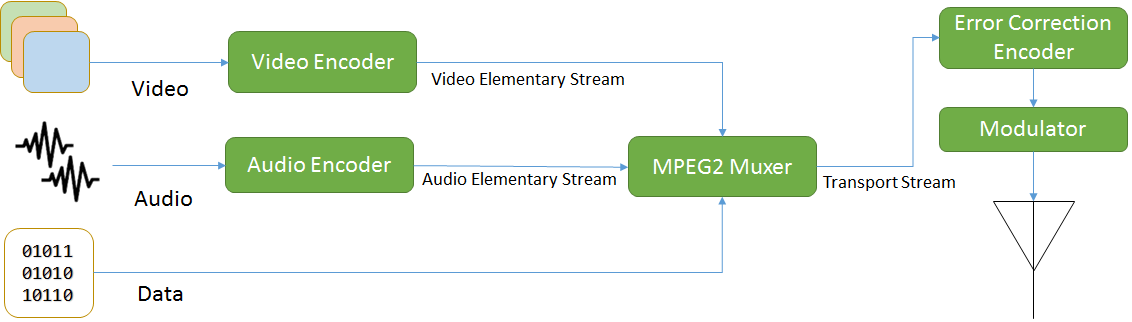
\includegraphics[width=1\linewidth]{figuras/diagrama_blocos_tvd.png}
\label{fig:diagrama_blocos_tvd}
\end{figure}
 
The main difference between analog and digital TV broadcasting systems, at the modulation level, is that in analog TV the multiplexing is in frequency domain, the video signal is sent in a frequency band within the channel bandwidth and the audio in another frequency band. In digital technology, this multiplexing happens in time domain: the multiplexer output has constant bitrate, and for fractions of second only one packet from one of the media sources is sent to the transmitter. In the other side of the channel, the receiver is conceived in such a way that after passing the error correction layer, a \textit{demultiplexer} takes the compound stream and splits it back into elementary bitstreams. They are then sent to the decoders and to audiovisual output devices.

It would be certainly disturbing to the viewer to watch delayed video or audio outputs, thus one challenge of this multiplexing scheme is to synchronize the reproduction of all the streams. To ensure this, presentation time stamps are added periodically into the streams so they can be reproduced in sync.

%O sistema de transmissão de televisão digital funciona, basicamente, coordenando a entrada de fluxos elementares de vídeo, áudio e dados no fluxo de transmissão. Na televisão analógica, a multiplexação é frequencial, ou seja, o sinal de vídeo é enviado em um intervalo de frequências dentro do canal e o sinal de áudio em outro intervalo. Na tecnologia digital, essa multiplexação é feita no tempo: por frações de segundo, apenas um dos sinais é enviado no canal e o receptor armazena os sinais independentemente para depois fazer a decodificação. No momento da reprodução dos sinais, é preciso que haja sincronismo nos fluxos de vídeo e áudio.

The Presitential Act number 8061\cite{decreto8061}, from july 29, 2013, establishes the chronogram of analog brodcasts shutdown. Until december 31, 2018, all analog transmitters shall be deactivated and the channels shall be vacated. The radio-frequency grants will then be returned to the government, that plans to use the 700MHz band to the 4G mobile telephone service, LTE.

%O Decreto presidencial número 8061, de 29 de julho de 2013, estabelece o cronograma de desligamento dos sistemas de transmissão de televisão analógica. Até 31 de dezembro de 2018, todos os transmissores analógicos devem ser desativados e os canais de radiofrequência devolvidos à união... COLOCAR REFERENCIA! 

The objective of this project is to develop a simple, yet flexible, tool to handle the Systems layer on SBTVD standard. Basically, by using this tool one is able to produce a SBTVD-compatible binary file containing a Transport Stream that can be used to broadcast recorded video and audio streams into appropriate receivers. Many commercial solutions for this objective are available on the market, so the target here was not to develop a consumer product, but rather something more academic, educational, where most of the configurations can be modified as desired. The main UFRGS internal client is the SBTVD set top box project, which is developing a set-top-box in as a System on Chip architecture in FPGA. In order to run tests of the entire system, streams with different multiplexing setups must be broadcast. When received, the way that the decoder handles them must be analysed.

The project work-flow was the following. The first step was to study the ABNT NBR15603 standard and the references in it to the ISO/IEC 13818 standard and to the ARIB STD-B10 standard. Here the target was to understand how the Systems Layer should work and identify which parts were mandatory and optional. While discussing the project at the very first weeks, it was decided to evaluate the possibility of develop the tool from scratch. This was before the first step was accomplished, because other people in the lab had already done some research and had concluded that the available freeware tools couldn't handle the SBTVD characteristics. During the author's own research on the Internet, some interesting tools were identified, and instead of developing from scratch, it seemed by then more reasonable to profit of an existent framework.

Once it was decided that an existing tool would be modified, the third step was to add the missing features in order to make it compatible with the SBTVD, and finally the features were tested on several receivers. The practical objective of the project is to provide a tool that creates Transport Streams with three key features: synchronous audiovisual presentation, compliance to the SBTVD standard and multiple services. Eventually, if any mandatory structures are only informational and do not block the system from working, they might be left for further development.

%In the first few weeks, no freeware solution had been found to meet these requirements, so it was proposed that the tool should be developed from scratch. After extra research efforts, some existing open source applications were found and fortunately they already met some of the requirements, but all were developed respecting the pure MPEG2 standard and naturally didn't include some of the brazilian system requirements. It was then proposed that the project target was to deliver no longer a solution from scratch, bu rather something based on one of the existing tools, adapting it to comprise the brazilian standard requirements. A discussion on the analysed tools is presented in the following chapters.

% The project objective is to develop an academic solution  not develop a customer solution, but rather an academic solution, in which one may broadcast streams without the restrictions of a commercial solution, although one may integrate the software to a modulator PCI board and a amplifier to constitute a small, cheap TV Station.

%In \autoref{codecs}, a brief description of the encoders chosen to integrate the standard is presented. In \autoref{}, 

%% FIM DA INTRODUÇÃO ESCRITA PARA O TCC

% ----------------------------------------------------------
% PARTE
% ----------------------------------------------------------
%\part{Preparação da pesquisa}
% ----------------------------------------------------------

% ---
% Capitulo com exemplos de comandos inseridos de arquivo externo 
% ---
%%% abtex2-modelo-include-comandos.tex, v-1.9.2 laurocesar
%% Copyright 2012-2014 by abnTeX2 group at http://abntex2.googlecode.com/ 
%%
%% This work may be distributed and/or modified under the
%% conditions of the LaTeX Project Public License, either version 1.3
%% of this license or (at your option) any later version.
%% The latest version of this license is in
%%   http://www.latex-project.org/lppl.txt
%% and version 1.3 or later is part of all distributions of LaTeX
%% version 2005/12/01 or later.
%%
%% This work has the LPPL maintenance status `maintained'.
%% 
%% The Current Maintainer of this work is the abnTeX2 team, led
%% by Lauro César Araujo. Further information are available on 
%% http://abntex2.googlecode.com/
%%
%% This work consists of the files abntex2-modelo-include-comandos.tex
%% and abntex2-modelo-img-marca.pdf
%%

% ---
% Este capítulo, utilizado por diferentes exemplos do abnTeX2, ilustra o uso de
% comandos do abnTeX2 e de LaTeX.
% ---
 
\chapter{Resultados de comandos}\label{cap_exemplos}

\chapterprecis{Isto é uma sinopse de capítulo. A ABNT não traz nenhuma
normatização a respeito desse tipo de resumo, que é mais comum em romances 
e livros técnicos.}\index{sinopse de capítulo}

% ---
\section{Codificação dos arquivos: UTF8}
% ---

A codificação de todos os arquivos do \abnTeX\ é \texttt{UTF8}. É necessário que
você utilize a mesma codificação nos documentos que escrever, inclusive nos
arquivos de base bibliográficas |.bib|.

% ---
\section{Citações diretas}
\label{sec-citacao}
% ---

\index{citações!diretas}Utilize o ambiente \texttt{citacao} para incluir
citações diretas com mais de três linhas:

\begin{citacao}
As citações diretas, no texto, com mais de três linhas, devem ser
destacadas com recuo de 4 cm da margem esquerda, com letra menor que a do texto
utilizado e sem as aspas. No caso de documentos datilografados, deve-se
observar apenas o recuo \cite[5.3]{NBR10520:2002}.
\end{citacao}

Use o ambiente assim:

\begin{verbatim}
\begin{citacao}
As citações diretas, no texto, com mais de três linhas [...] deve-se observar
apenas o recuo \cite[5.3]{NBR10520:2002}.
\end{citacao}
\end{verbatim}

O ambiente \texttt{citacao} pode receber como parâmetro opcional um nome de
idioma previamente carregado nas opções da classe (\autoref{sec-hifenizacao}). Nesse
caso, o texto da citação é automaticamente escrito em itálico e a hifenização é
ajustada para o idioma selecionado na opção do ambiente. Por exemplo:

\begin{verbatim}
\begin{citacao}[english]
Text in English language in italic with correct hyphenation.
\end{citacao}
\end{verbatim}

Tem como resultado:

\begin{citacao}[english]
Text in English language in italic with correct hyphenation.
\end{citacao}

\index{citações!simples}Citações simples, com até três linhas, devem ser
incluídas com aspas. Observe que em \LaTeX as aspas iniciais são diferentes das
finais: ``Amor é fogo que arde sem se ver''.

% ---
\section{Notas de rodapé}
% ---

As notas de rodapé são detalhadas pela NBR 14724:2011 na seção 5.2.1\footnote{As
notas devem ser digitadas ou datilografadas dentro das margens, ficando
separadas do texto por um espaço simples de entre as linhas e por filete de 5
cm, a partir da margem esquerda. Devem ser alinhadas, a partir da segunda linha
da mesma nota, abaixo da primeira letra da primeira palavra, de forma a destacar
o expoente, sem espaço entre elas e com fonte menor
\citeonline[5.2.1]{NBR14724:2011}.}\footnote{Caso uma série de notas sejam
criadas sequencialmente, o \abnTeX\ instrui o \LaTeX\ para que uma vírgula seja
colocada após cada número do expoente que indica a nota de rodapé no corpo do
texto.}\footnote{Verifique se os números do expoente possuem uma vírgula para
dividi-los no corpo do texto.}. 


% ---
\section{Tabelas}
% ---

\index{tabelas}A \autoref{tab-nivinv} é um exemplo de tabela construída em
\LaTeX.

\begin{table}[htb]
\ABNTEXfontereduzida
\caption[Níveis de investigação]{Níveis de investigação.}
\label{tab-nivinv}
\begin{tabular}{p{2.6cm}|p{6.0cm}|p{2.25cm}|p{3.40cm}}
  %\hline
   \textbf{Nível de Investigação} & \textbf{Insumos}  & \textbf{Sistemas de Investigação}  & \textbf{Produtos}  \\
    \hline
    Meta-nível & Filosofia\index{filosofia} da Ciência  & Epistemologia &
    Paradigma  \\
    \hline
    Nível do objeto & Paradigmas do metanível e evidências do nível inferior &
    Ciência  & Teorias e modelos \\
    \hline
    Nível inferior & Modelos e métodos do nível do objeto e problemas do nível inferior & Prática & Solução de problemas  \\
   % \hline
\end{tabular}
\legend{Fonte: \citeonline{van86}}
\end{table}

Já a \autoref{tabela-ibge} apresenta uma tabela criada conforme o padrão do
\citeonline{ibge1993} requerido pelas normas da ABNT para documentos técnicos e
acadêmicos.

\begin{table}[htb]
\IBGEtab{%
  \caption{Um Exemplo de tabela alinhada que pode ser longa
  ou curta, conforme padrão IBGE.}%
  \label{tabela-ibge}
}{%
  \begin{tabular}{ccc}
  \toprule
   Nome & Nascimento & Documento \\
  \midrule \midrule
   Maria da Silva & 11/11/1111 & 111.111.111-11 \\
  \midrule 
   João Souza & 11/11/2111 & 211.111.111-11 \\
  \midrule 
   Laura Vicuña & 05/04/1891 & 3111.111.111-11 \\
  \bottomrule
\end{tabular}%
}{%
  \fonte{Produzido pelos autores.}%
  \nota{Esta é uma nota, que diz que os dados são baseados na
  regressão linear.}%
  \nota[Anotações]{Uma anotação adicional, que pode ser seguida de várias
  outras.}%
  }
\end{table}


% ---
\section{Figuras}
% ---

\index{figuras}Figuras podem ser criadas diretamente em \LaTeX,
como o exemplo da \autoref{fig_circulo}.

\begin{figure}[htb]
	\caption{\label{fig_circulo}A delimitação do espaço}
	\begin{center}
	    \setlength{\unitlength}{5cm}
		\begin{picture}(1,1)
		\put(0,0){\line(0,1){1}}
		\put(0,0){\line(1,0){1}}
		\put(0,0){\line(1,1){1}}
		\put(0,0){\line(1,2){.5}}
		\put(0,0){\line(1,3){.3333}}
		\put(0,0){\line(1,4){.25}}
		\put(0,0){\line(1,5){.2}}
		\put(0,0){\line(1,6){.1667}}
		\put(0,0){\line(2,1){1}}
		\put(0,0){\line(2,3){.6667}}
		\put(0,0){\line(2,5){.4}}
		\put(0,0){\line(3,1){1}}
		\put(0,0){\line(3,2){1}}
		\put(0,0){\line(3,4){.75}}
		\put(0,0){\line(3,5){.6}}
		\put(0,0){\line(4,1){1}}
		\put(0,0){\line(4,3){1}}
		\put(0,0){\line(4,5){.8}}
		\put(0,0){\line(5,1){1}}
		\put(0,0){\line(5,2){1}}
		\put(0,0){\line(5,3){1}}
		\put(0,0){\line(5,4){1}}
		\put(0,0){\line(5,6){.8333}}
		\put(0,0){\line(6,1){1}}
		\put(0,0){\line(6,5){1}}
		\end{picture}
	\end{center}
	\legend{Fonte: os autores}
\end{figure}

Ou então figuras podem ser incorporadas de arquivos externos, como é o caso da
\autoref{fig_grafico}. Se a figura que ser incluída se tratar de um diagrama, um
gráfico ou uma ilustração que você mesmo produza, priorize o uso de imagens
vetoriais no formato PDF. Com isso, o tamanho do arquivo final do trabalho será
menor, e as imagens terão uma apresentação melhor, principalmente quando
impressas, uma vez que imagens vetorias são perfeitamente escaláveis para
qualquer dimensão. Nesse caso, se for utilizar o Microsoft Excel para produzir
gráficos, ou o Microsoft Word para produzir ilustrações, exporte-os como PDF e
os incorpore ao documento conforme o exemplo abaixo. No entanto, para manter a
coerência no uso de software livre (já que você está usando \LaTeX e \abnTeX),
teste a ferramenta \textsf{InkScape}\index{InkScape}
(\url{http://inkscape.org/}). Ela é uma excelente opção de código-livre para
produzir ilustrações vetoriais, similar ao CorelDraw\index{CorelDraw} ou ao Adobe
Illustrator\index{Adobe Illustrator}. De todo modo, caso não seja possível
utilizar arquivos de imagens como PDF, utilize qualquer outro formato, como
JPEG, GIF, BMP, etc. Nesse caso, você pode tentar aprimorar as imagens
incorporadas com o software livre \textsf{Gimp}\index{Gimp}
(\url{http://www.gimp.org/}). Ele é uma alternativa livre ao Adobe
Photoshop\index{Adobe Photoshop}.

\begin{figure}[htb]
	\caption{\label{fig_grafico}Gráfico produzido em Excel e salvo como PDF}
	\begin{center}
	    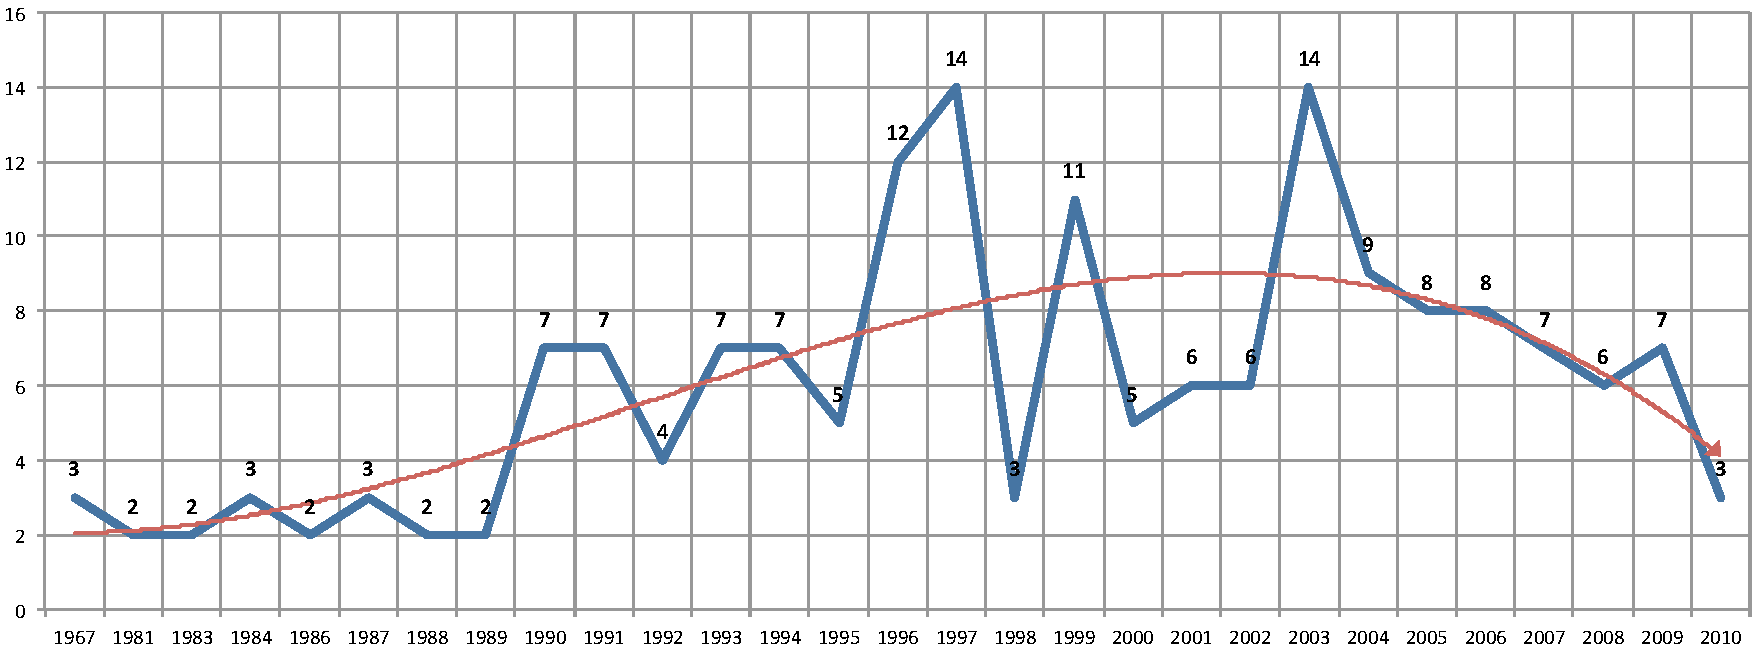
\includegraphics[scale=0.5]{abntex2-modelo-img-grafico.pdf}
	\end{center}
	\legend{Fonte: \citeonline[p. 24]{araujo2012}}
\end{figure}

% ---
\subsection{Figuras em \emph{minipages}}
% ---

\emph{Minipages} são usadas para inserir textos ou outros elementos em quadros
com tamanhos e posições controladas. Veja o exemplo da
\autoref{fig_minipage_imagem1} e da \autoref{fig_minipage_grafico2}.

\begin{figure}[htb]
 \label{teste}
 \centering
  \begin{minipage}{0.4\textwidth}
    \centering
    \caption{Imagem 1 da minipage} \label{fig_minipage_imagem1}
    
\includegraphics[scale=0.9]{abntex2-modelo-img-marca.pdf}
    \legend{Fonte: Produzido pelos autores}
  \end{minipage}
  \hfill
  \begin{minipage}{0.4\textwidth}
    \centering
    \caption{Grafico 2 da minipage} \label{fig_minipage_grafico2}
    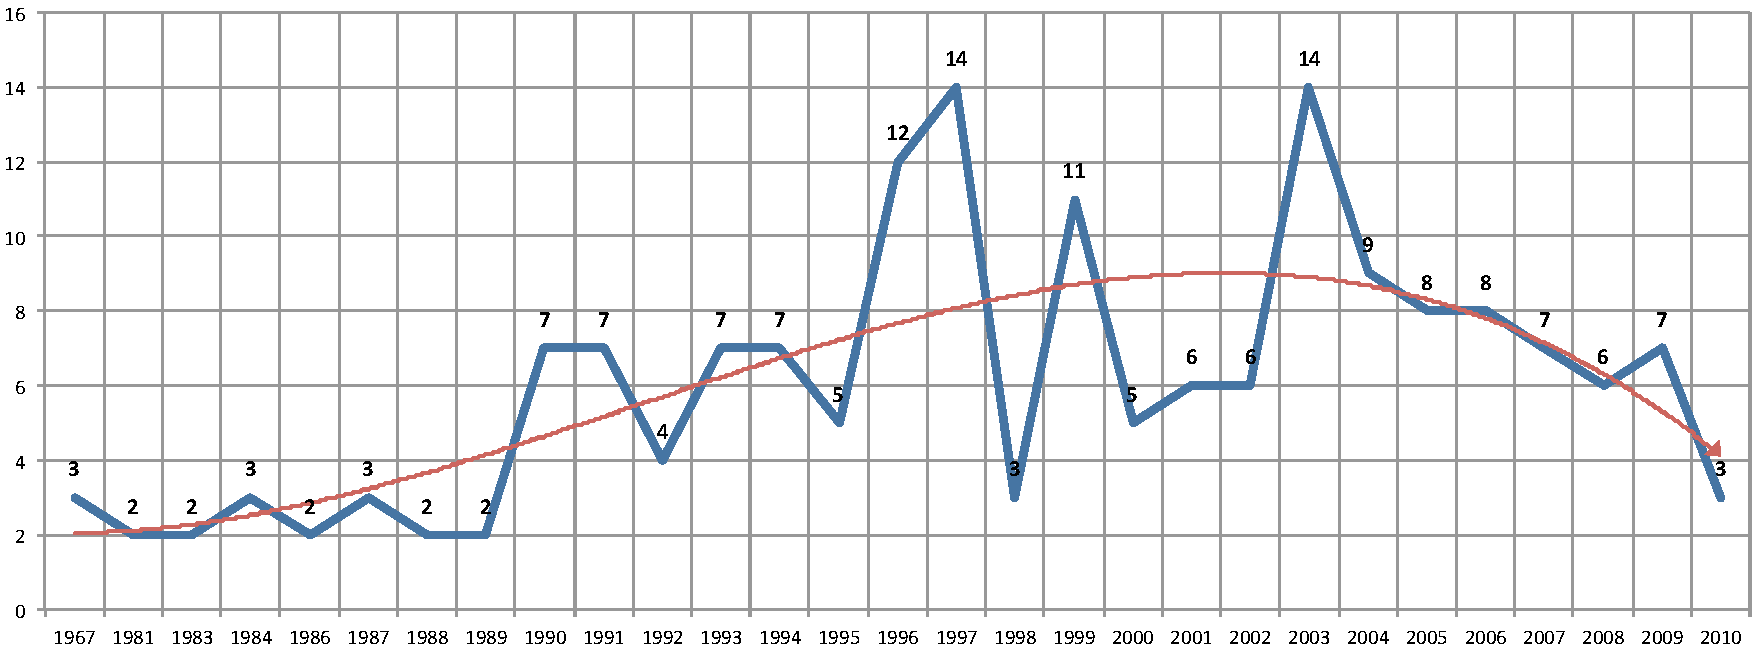
\includegraphics[scale=0.2]{abntex2-modelo-img-grafico.pdf}
    \legend{Fonte: \citeonline[p. 24]{araujo2012}}
  \end{minipage}
\end{figure}

Observe que, segundo a \citeonline[seções 4.2.1.10 e 5.8]{NBR14724:2011}, as
ilustrações devem sempre ter numeração contínua e única em todo o documento:

\begin{citacao}
Qualquer que seja o tipo de ilustração, sua identificação aparece na parte
superior, precedida da palavra designativa (desenho, esquema, fluxograma,
fotografia, gráfico, mapa, organograma, planta, quadro, retrato, figura,
imagem, entre outros), seguida de seu número de ordem de ocorrência no texto,
em algarismos arábicos, travessão e do respectivo título. Após a ilustração, na
parte inferior, indicar a fonte consultada (elemento obrigatório, mesmo que
seja produção do próprio autor), legenda, notas e outras informações
necessárias à sua compreensão (se houver). A ilustração deve ser citada no
texto e inserida o mais próximo possível do trecho a que se
refere. \cite[seções 5.8]{NBR14724:2011}
\end{citacao}

% ---
\section{Expressões matemáticas}
% ---

\index{expressões matemáticas}Use o ambiente \texttt{equation} para escrever
expressões matemáticas numeradas:

\begin{equation}
  \forall x \in X, \quad \exists \: y \leq \epsilon
\end{equation}

Escreva expressões matemáticas entre \$ e \$, como em $ \lim_{x \to \infty}
\exp(-x) = 0 $, para que fiquem na mesma linha.

Também é possível usar colchetes para indicar o início de uma expressão
matemática que não é numerada.

\[
\left|\sum_{i=1}^n a_ib_i\right|
\le
\left(\sum_{i=1}^n a_i^2\right)^{1/2}
\left(\sum_{i=1}^n b_i^2\right)^{1/2}
\]

Consulte mais informações sobre expressões matemáticas em
\url{https://code.google.com/p/abntex2/wiki/Referencias}.

% ---
\section{Enumerações: alíneas e subalíneas}
% ---

\index{alíneas}\index{subalíneas}\index{incisos}Quando for necessário enumerar
os diversos assuntos de uma seção que não possua título, esta deve ser
subdividida em alíneas \cite[4.2]{NBR6024:2012}:

\begin{alineas}

  \item os diversos assuntos que não possuam título próprio, dentro de uma mesma
  seção, devem ser subdivididos em alíneas; 
  
  \item o texto que antecede as alíneas termina em dois pontos;
  \item as alíneas devem ser indicadas alfabeticamente, em letra minúscula,
  seguida de parêntese. Utilizam-se letras dobradas, quando esgotadas as
  letras do alfabeto;

  \item as letras indicativas das alíneas devem apresentar recuo em relação à
  margem esquerda;

  \item o texto da alínea deve começar por letra minúscula e terminar em
  ponto-e-vírgula, exceto a última alínea que termina em ponto final;

  \item o texto da alínea deve terminar em dois pontos, se houver subalínea;

  \item a segunda e as seguintes linhas do texto da alínea começa sob a
  primeira letra do texto da própria alínea;
  
  \item subalíneas \cite[4.3]{NBR6024:2012} devem ser conforme as alíneas a
  seguir:

  \begin{alineas}
     \item as subalíneas devem começar por travessão seguido de espaço;

     \item as subalíneas devem apresentar recuo em relação à alínea;

     \item o texto da subalínea deve começar por letra minúscula e terminar em
     ponto-e-vírgula. A última subalínea deve terminar em ponto final, se não
     houver alínea subsequente;

     \item a segunda e as seguintes linhas do texto da subalínea começam sob a
     primeira letra do texto da própria subalínea.
  \end{alineas}
  
  \item no \abnTeX\ estão disponíveis os ambientes \texttt{incisos} e
  \texttt{subalineas}, que em suma são o mesmo que se criar outro nível de
  \texttt{alineas}, como nos exemplos à seguir:
  
  \begin{incisos}
    \item \textit{Um novo inciso em itálico};
  \end{incisos}
  
  \item Alínea em \textbf{negrito}:
  
  \begin{subalineas}
    \item \textit{Uma subalínea em itálico};
    \item \underline{\textit{Uma subalínea em itálico e sublinhado}}; 
  \end{subalineas}
  
  \item Última alínea com \emph{ênfase}.
  
\end{alineas}

% ---
\section{Espaçamento entre parágrafos e linhas}
% ---

\index{espaçamento!dos parágrafos}O tamanho do parágrafo, espaço entre a margem
e o início da frase do parágrafo, é definido por:

\begin{verbatim}
   \setlength{\parindent}{1.3cm}
\end{verbatim}

\index{espaçamento!do primeiro parágrafo}Por padrão, não há espaçamento no
primeiro parágrafo de cada início de divisão do documento
(\autoref{sec-divisoes}). Porém, você pode definir que o primeiro parágrafo
também seja indentado, como é o caso deste documento. Para isso, apenas inclua o
pacote \textsf{indentfirst} no preâmbulo do documento:

\begin{verbatim}
   \usepackage{indentfirst}      % Indenta o primeiro parágrafo de cada seção.
\end{verbatim}

\index{espaçamento!entre os parágrafos}O espaçamento entre um parágrafo e outro
pode ser controlado por meio do comando:

\begin{verbatim}
  \setlength{\parskip}{0.2cm}  % tente também \onelineskip
\end{verbatim}

\index{espaçamento!entre as linhas}O controle do espaçamento entre linhas é
definido por:

\begin{verbatim}
  \OnehalfSpacing       % espaçamento um e meio (padrão); 
  \DoubleSpacing        % espaçamento duplo
  \SingleSpacing        % espaçamento simples	
\end{verbatim}

Para isso, também estão disponíveis os ambientes:

\begin{verbatim}
  \begin{SingleSpace} ...\end{SingleSpace}
  \begin{Spacing}{hfactori} ... \end{Spacing}
  \begin{OnehalfSpace} ... \end{OnehalfSpace}
  \begin{OnehalfSpace*} ... \end{OnehalfSpace*}
  \begin{DoubleSpace} ... \end{DoubleSpace}
  \begin{DoubleSpace*} ... \end{DoubleSpace*} 
\end{verbatim}

Para mais informações, consulte \citeonline[p. 47-52 e 135]{memoir}.

% ---
\section{Inclusão de outros arquivos}\label{sec-include}
% ---

É uma boa prática dividir o seu documento em diversos arquivos, e não
apenas escrever tudo em um único. Esse recurso foi utilizado neste
documento. Para incluir diferentes arquivos em um arquivo principal,
de modo que cada arquivo incluído fique em uma página diferente, utilize o
comando:

\begin{verbatim}
   \include{documento-a-ser-incluido}      % sem a extensão .tex
\end{verbatim}

Para incluir documentos sem quebra de páginas, utilize:

\begin{verbatim}
   \input{documento-a-ser-incluido}      % sem a extensão .tex
\end{verbatim}

% ---
\section{Compilar o documento \LaTeX}
% ---

Geralmente os editores \LaTeX, como o
TeXlipse\footnote{\url{http://texlipse.sourceforge.net/}}, o
Texmaker\footnote{\url{http://www.xm1math.net/texmaker/}}, entre outros,
compilam os documentos automaticamente, de modo que você não precisa se
preocupar com isso.

No entanto, você pode compilar os documentos \LaTeX usando os seguintes
comandos, que devem ser digitados no \emph{Prompt de Comandos} do Windows ou no
\emph{Terminal} do Mac ou do Linux:

\begin{verbatim}
   pdflatex ARQUIVO_PRINCIPAL.tex
   bibtex ARQUIVO_PRINCIPAL.aux
   makeindex ARQUIVO_PRINCIPAL.idx 
   makeindex ARQUIVO_PRINCIPAL.nlo -s nomencl.ist -o ARQUIVO_PRINCIPAL.nls
   pdflatex ARQUIVO_PRINCIPAL.tex
   pdflatex ARQUIVO_PRINCIPAL.tex
\end{verbatim}

% ---
\section{Remissões internas}
% ---

Ao nomear a \autoref{tab-nivinv} e a \autoref{fig_circulo}, apresentamos um
exemplo de remissão interna, que também pode ser feita quando indicamos o
\autoref{cap_exemplos}, que tem o nome \emph{\nameref{cap_exemplos}}. O número
do capítulo indicado é \ref{cap_exemplos}, que se inicia à
\autopageref{cap_exemplos}\footnote{O número da página de uma remissão pode ser
obtida também assim:
\pageref{cap_exemplos}.}.
Veja a \autoref{sec-divisoes} para outros exemplos de remissões internas entre
seções, subseções e subsubseções.

O código usado para produzir o texto desta seção é:

\begin{verbatim}
Ao nomear a \autoref{tab-nivinv} e a \autoref{fig_circulo}, apresentamos um
exemplo de remissão interna, que também pode ser feita quando indicamos o
\autoref{cap_exemplos}, que tem o nome \emph{\nameref{cap_exemplos}}. O número
do capítulo indicado é \ref{cap_exemplos}, que se inicia à
\autopageref{cap_exemplos}\footnote{O número da página de uma remissão pode ser
obtida também assim:
\pageref{cap_exemplos}.}.
Veja a \autoref{sec-divisoes} para outros exemplos de remissões internas entre
seções, subseções e subsubseções.
\end{verbatim}

% ---
\section{Divisões do documento: seção}\label{sec-divisoes}
% ---

Esta seção testa o uso de divisões de documentos. Esta é a
\autoref{sec-divisoes}. Veja a \autoref{sec-divisoes-subsection}.

\subsection{Divisões do documento: subseção}\label{sec-divisoes-subsection}

Isto é uma subseção. Veja a \autoref{sec-divisoes-subsubsection}, que é uma
\texttt{subsubsection} do \LaTeX, mas é impressa chamada de ``subseção'' porque
no Português não temos a palavra ``subsubseção''.

\subsubsection{Divisões do documento: subsubseção}
\label{sec-divisoes-subsubsection}

Isto é uma subsubseção.

\subsubsection{Divisões do documento: subsubseção}

Isto é outra subsubseção.

\subsection{Divisões do documento: subseção}\label{sec-exemplo-subsec}

Isto é uma subseção.

\subsubsection{Divisões do documento: subsubseção}

Isto é mais uma subsubseção da \autoref{sec-exemplo-subsec}.


\subsubsubsection{Esta é uma subseção de quinto
nível}\label{sec-exemplo-subsubsubsection}

Esta é uma seção de quinto nível. Ela é produzida com o seguinte comando:

\begin{verbatim}
\subsubsubsection{Esta é uma subseção de quinto
nível}\label{sec-exemplo-subsubsubsection}
\end{verbatim}

\subsubsubsection{Esta é outra subseção de quinto nível}\label{sec-exemplo-subsubsubsection-outro}

Esta é outra seção de quinto nível.


\paragraph{Este é um parágrafo numerado}\label{sec-exemplo-paragrafo}

Este é um exemplo de parágrafo nomeado. Ele é produzida com o comando de
parágrafo:

\begin{verbatim}
\paragraph{Este é um parágrafo nomeado}\label{sec-exemplo-paragrafo}
\end{verbatim}

A numeração entre parágrafos numeradaos e subsubsubseções são contínuas.

\paragraph{Esta é outro parágrafo numerado}\label{sec-exemplo-paragrafo-outro}

Esta é outro parágrafo nomeado.

% ---
\section{Este é um exemplo de nome de seção longo. Ele deve estar
alinhado à esquerda e a segunda e demais linhas devem iniciar logo abaixo da
primeira palavra da primeira linha}
% ---

Isso atende à norma \citeonline[seções de 5.2.2 a 5.2.4]{NBR14724:2011} 
 e \citeonline[seções de 3.1 a 3.8]{NBR6024:2012}.

% ---
\section{Diferentes idiomas e hifenizações}
\label{sec-hifenizacao}
% ---

Para usar hifenizações de diferentes idiomas, inclua nas opções do documento o
nome dos idiomas que o seu texto contém. Por exemplo (para melhor
visualização, as opções foram quebras em diferentes linhas):

\begin{verbatim}
\documentclass[
	12pt,
	openright,
	twoside,
	a4paper,
	english,
	french,
	spanish,
	brazil
	]{abntex2}
\end{verbatim}

O idioma português-brasileiro (\texttt{brazil}) é incluído automaticamente pela
classe \textsf{abntex2}. Porém, mesmo assim a opção \texttt{brazil} deve ser
informada como a última opção da classe para que todos os pacotes reconheçam o
idioma. Vale ressaltar que a última opção de idioma é a utilizada por padrão no
documento. Desse modo, caso deseje escrever um texto em inglês que tenha
citações em português e em francês, você deveria usar o preâmbulo como abaixo:

\begin{verbatim}
\documentclass[
	12pt,
	openright,
	twoside,
	a4paper,
	french,
	brazil,
	english
	]{abntex2}
\end{verbatim}

A lista completa de idiomas suportados, bem como outras opções de hifenização,
estão disponíveis em \citeonline[p.~5-6]{babel}.

Exemplo de hifenização em inglês\footnote{Extraído de:
\url{http://en.wikibooks.org/wiki/LaTeX/Internationalization}}:

\begin{otherlanguage*}{english}
\textit{Text in English language. This environment switches all language-related
definitions, like the language specific names for figures, tables etc. to the other
language. The starred version of this environment typesets the main text
according to the rules of the other language, but keeps the language specific
string for ancillary things like figures, in the main language of the document.
The environment hyphenrules switches only the hyphenation patterns used; it can
also be used to disallow hyphenation by using the language name
`nohyphenation'.}
\end{otherlanguage*}

Exemplo de hifenização em francês\footnote{Extraído de:
\url{http://bigbrowser.blog.lemonde.fr/2013/02/17/tu-ne-tweeteras-point-le-vatican-interdit-aux-cardinaux-de-tweeter-pendant-le-conclave/}}:

\begin{otherlanguage*}{french}
\textit{Texte en français. Pas question que Twitter ne vienne faire une
concurrence déloyale à la traditionnelle fumée blanche qui marque l'élection
d'un nouveau pape. Pour éviter toute fuite précoce, le Vatican a donc pris un
peu d'avance, et a déjà interdit aux cardinaux qui prendront part au vote
d'utiliser le réseau social, selon Catholic News Service. Une mesure valable
surtout pour les neuf cardinaux – sur les 117 du conclave – pratiquants très
actifs de Twitter, qui auront interdiction pendant toute la période de se
connecter à leur compte.}
\end{otherlanguage*}

Pequeno texto em espanhol\footnote{Extraído de:
\url{http://internacional.elpais.com/internacional/2013/02/17/actualidad/1361102009_913423.html}}:

\foreignlanguage{spanish}{\textit{Decenas de miles de personas ovacionan al pontífice en su
penúltimo ángelus dominical, el primero desde que anunciase su renuncia. El Papa se
centra en la crítica al materialismo}}.

O idioma geral do texto por ser alterado como no exemplo seguinte:

\begin{verbatim}
  \selectlanguage{english}
\end{verbatim}

Isso altera automaticamente a hifenização e todos os nomes constantes de
referências do documento para o idioma inglês. Consulte o manual da classe
\cite{abntex2classe} para obter orientações adicionais sobre internacionalização de
documentos produzidos com \abnTeX.

A \autoref{sec-citacao} descreve o ambiente \texttt{citacao} que pode receber
como parâmetro um idioma a ser usado na citação.

% ---
\section{Consulte o manual da classe \textsf{abntex2}}
% ---

Consulte o manual da classe \textsf{abntex2} \cite{abntex2classe} para uma
referência completa das macros e ambientes disponíveis. 

Além disso, o manual possui informações adicionais sobre as normas ABNT
observadas pelo \abnTeX\ e considerações sobre eventuais requisitos específicos
não atendidos, como o caso da \citeonline[seção 5.2.2]{NBR14724:2011}, que
especifica o espaçamento entre os capítulos e o início do texto, regra
propositalmente não atendida pelo presente modelo.

% ---
\section{Referências bibliográficas}
% ---

A formatação das referências bibliográficas conforme as regras da ABNT são um
dos principais objetivos do \abnTeX. Consulte os manuais
\citeonline{abntex2cite} e \citeonline{abntex2cite-alf} para obter informações
sobre como utilizar as referências bibliográficas.

%-
\subsection{Acentuação de referências bibliográficas}
%-

Normalmente não há problemas em usar caracteres acentuados em arquivos
bibliográficos (\texttt{*.bib}). Porém, como as regras da ABNT fazem uso quase
abusivo da conversão para letras maiúsculas, é preciso observar o modo como se
escreve os nomes dos autores. Na ~\autoref{tabela-acentos} você encontra alguns
exemplos das conversões mais importantes. Preste atenção especial para `ç' e `í'
que devem estar envoltos em chaves. A regra geral é sempre usar a acentuação
neste modo quando houver conversão para letras maiúsculas.

\begin{table}[htbp]
\caption{Tabela de conversão de acentuação.}
\label{tabela-acentos}

\begin{center}
\begin{tabular}{ll}\hline\hline
acento & \textsf{bibtex}\\
à á ã & \verb+\`a+ \verb+\'a+ \verb+\~a+\\
í & \verb+{\'\i}+\\
ç & \verb+{\c c}+\\
\hline\hline
\end{tabular}
\end{center}
\end{table}


% ---
\section{Precisa de ajuda?}
% ---

Consulte a FAQ com perguntas frequentes e comuns no portal do \abnTeX:
\url{https://code.google.com/p/abntex2/wiki/FAQ}.

Inscreva-se no grupo de usuários \LaTeX:
\url{http://groups.google.com/group/latex-br}, tire suas dúvidas e ajude
outros usuários.

Participe também do grupo de desenvolvedores do \abnTeX:
\url{http://groups.google.com/group/abntex2} e faça sua contribuição à
ferramenta.

% ---
\section{Você pode ajudar?}
% ---

Sua contribuição é muito importante! Você pode ajudar na divulgação, no
desenvolvimento e de várias outras formas. Veja como contribuir com o \abnTeX\
em \url{https://code.google.com/p/abntex2/wiki/ComoContribuir}.

% ---
\section{Quer customizar os modelos do \abnTeX\ para sua instituição ou
universidade?}
% ---

Veja como customizar o \abnTeX\ em:
\url{https://code.google.com/p/abntex2/wiki/ComoCustomizar}.


% ---

% ----------------------------------------------------------
% PARTE
% ----------------------------------------------------------
%\part{Referenciais teóricos}
% ----------------------------------------------------------

% ---
% Capitulo de revisão de literatura
% ---

\chapter{Audiovisual codecs used in SBTVD}
\label{codecs}

The codecs chosen to be used in SBTVD are H.264 for video and AAC/LATM for the audio. This overview is useful to understand the synchronization methods adopted in the systems layer, explained further in the text.

\section{H.264}

The H.264 video coding standard is also known as the MPEG-4 Part 10 standard, and it was published as the evolution of the existing video coding standards (ITU-T H.261 / MPEG1, ITU-T H.262 / MPEG2). The main applications for this standard, as described by the publisher itself, are video-conferencing, digital  media storage, television broadcasting, Internet streaming and Internet communication. It was developed to provide a solution that has higher compression rates than the former standards, and yet improves subjective quality. To the television broadcast market, it suits perfectly the transmission of high definition video. Technically, the encoder takes the raw video frames and sequentially performs prediction, transform and entropy encoding processes to produce a compressed bitstream. The codec features are organized in profiles and levels, the \textit{high} profile suits the HDTV video transmission characteristics on the Full Segment transmission, while the \textit{baseline} profile fits the needs for mobile, 1-Segment broadcasts. See \autoref{modulation}.


In the first step, prediction, the encoder splits one frame into square or rectangular blocks of pixels, called macroblocks, and predicts the values of pixels in the current macroblock based on information from previously analysed macroblocks either in the current frame or in previously coded frames. Then, instead of transmitting the pixel values, is transmits the difference between the original and the predicted frame (which should have less information if the encoder is efficient) along with pointers to the macroblocks that must be used to recreate that region. These pointers are called motion vectors. There are three different types of prediction schemes, that lead to different kinds of frames:

\begin{itemize}
\item{an I-frame is constructed by predicting pixel values only from macroblocks within the same frame, this is the intra-frame prediction;}
\item{a P-frame is composed of predictions from the current source frame and also of the previously coded I-frame, this is the inter-frame prediction;}
\item{a B-frame is made by predicting the output frame from the current input, the earlier inputs or yet the later input frames, and is known as the bidirectional inter-frame prediction.}
\end{itemize}

The decrease in amount of information can be noticed in \autoref{fig:motion_compensation}, adapted from \cite{richardson}. The first frame is marked as (a) and coded with intra prediction. The following frame in presentation sequence is (b), which is coded as a P-frame. There is a slight difference between frames that can be seen by the bicycle position. When generic motion compensation coding is applied, the residual frame is the one in (c). Knowing that these frames have differential pixel values \footnote{Differential pixel values means that a black pixel is the negative threshold, a white pixel is the positive threshold and gray is zero.}, it can be noticed that most of the pixels have a value close to zero in (c), which means a residual with very little information. The number of bytes needed to code one I frame is therefore much higher than the necessary to code a P frame, since there is no motion compensation in the first one.

\begin{figure}
\centering
\caption{Visualization of motion compensation encoder working.}
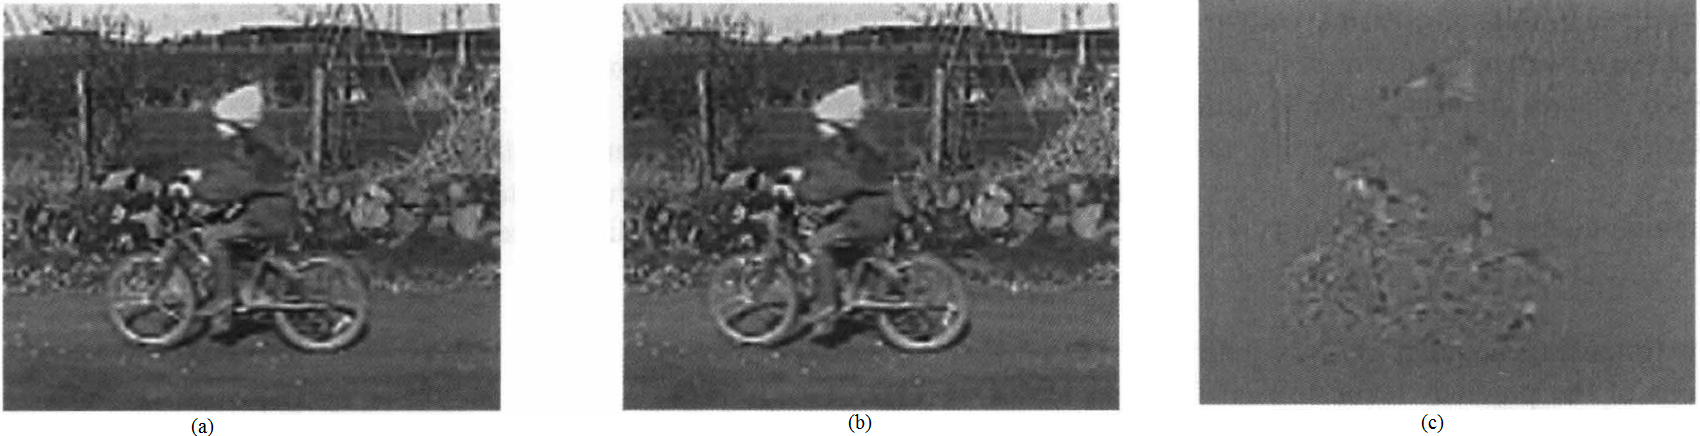
\includegraphics[width=1\linewidth]{figuras/motion_compensation.png}
\\Source: \cite{richardson}.
\label{fig:motion_compensation}
\end{figure}

Although there is a substantial decrease in amount of information with inter-frame prediction, the video quality may degenerate if too many P and B frames are used between two I frames, due to quantization. This leads to a compromise of quality and bitrate and the usual frame arrangement is the one shown in \autoref{fig:IBBPBBP}, that places at most two B frames between one I and one P, or between two P frames, and at most two P frames between consecutive I frames. This arrangement is called a Group of Pictures, or GOP as referenced in MPEG4 standard.

\begin{figure}
\centering
\caption{Usual group of pictures arrangement.}
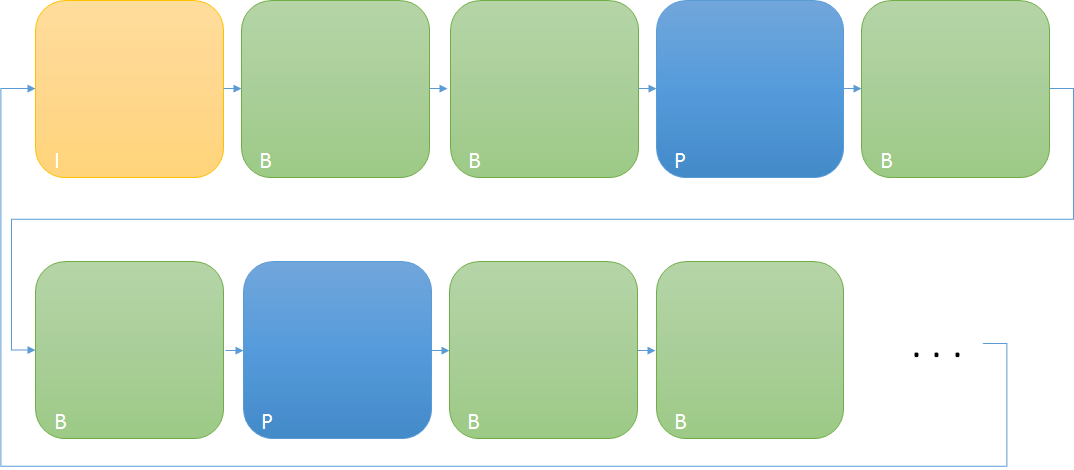
\includegraphics[width=0.6\linewidth]{figuras/IBBPBBP.png}
\\Source: The Author.
\label{fig:IBBPBBP}
\end{figure}

The next encoder step is to transform the residual frame from prediction with an integer approximation of the Discrete Cosine Transform, or DCT, so that the pixel values become a set of frequency domain coefficients. These coefficients are then quantized, which reduce their precision and make many of them to be equal to zero. Finally, the coefficients are reordered to align most of the zero-valued ones consecutively, and an entropy encoder reduces the redundancy of the sequences of repetitions, hence reducing the amount of data. The output of the H.264 encoder is formed of the quantized coefficients and the motion vectors arranged in a structured bitstream, that constitutes the video Elementary Stream. Further information can be found in \cite{vcodex} or \cite{richardson}.

\section{AAC}

The audio codec chosen to incorporate the SBTVD, developed by Fraunhofer IIS along with AT\&T, Dolby and Sony, is called Advanced Audio Coding, or AAC. Since the beginning of the development in 1994, the successive evolutions in the codec gave place to profiles that assemble the main features. Three different profiles are the mostly used in digital television broadcast: AAC-LC, HE-AAC, HE-AACv2. According to the main developer\cite{fraunhofer}, even the simplest profile, AAC-LC (LC for low complexity) provides \textit{"an audio whose quality even for expert listeners, so-called golden ears, is indistinguishable from the original"}.

The codec supports encoding of ancillary data along with the audio samples, and all with typically 192Kbps for broadcast quality stereo streams in AAC-LC profile. If the HE-AAC profile is chosen, the Spectral Band Replication(SBR) feature is applied and for the same audio quality in the output, a 30\% bitrate reduction is observed. In HE-AAC the lower part of the audio spectrum is sampled at half the frequency of the remaining signal using AAC-LC, and the high frequency band is coded with SBR. SBR exploits the relationship of upper and lower sides of the spectrum to produce a parametric recreation of the upper band, thus reducing the total bitrate. HE-AAC achieves typical 48 to 64 kbps for stereo streams.

The chosen profile to integrate the SBTVD is HE-AACv2. Additionally to the already described features, it includes the Parametric Stereo (PS) tool. Rather than encoding two separate channels without any relationship between them, PS creates a monaural downmix of the two stereo samples and a set of parametric coefficients. The mono stream is then encoded with HE-AAC and sent along with the coefficients to recreate stereo sound in the receiver side. Finally, with both PS and SBR, the bitrate is reduced even more, to up to 24 Kbps for stereo audio. \autoref{fig:he_aac_v2} presents the encoding and decoding processes for HE-AACv2 profile. The audio stream enters the encoder and reaches first the Parametric Stereo step. The set of coefficients are extracted, injected as ancillary data and the residual enters both the SBR encoder and the downsampler. The SBR coefficients are calculated and added to the ancillary data, and the final residual is coded with AAC-LC.

\begin{figure}
\centering
\caption{Block diagram of HE-AACv2 profile encoding and decoding steps.}
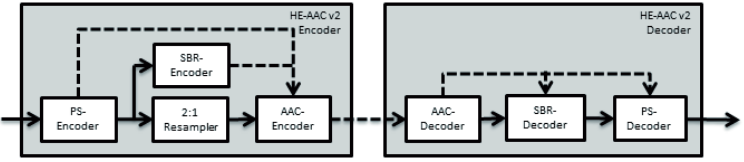
\includegraphics[width=1\linewidth]{figuras/he_aac_v2.png}
\\Source and Copyright: \cite{fraunhofer}.
\label{fig:he_aac_v2}
\end{figure}

LATM is the selected method for encapsulating audio frames for transmission in SBTVD Transport Streams. Further information can be obtained in ISO/IEC 14496-3 International Standard - Audio.

\chapter{ISO/IEC 13818-1 Standard}
\label{iso13818}
% ---
The main objective of the ISO/IEC13818-1 standard is to describe the conversion of multiple bitstreams into one single stream carrying wrapped video and audio data, as well as additional information responsible to unwrap the streams. Similarly to other ISO/IEC standards, the text only specifies the decoding/demultiplexing side of the transmission chain, leaving the architectures of encoding/multiplexing stages to the manufacturers decision.

Some concepts should be briefly described to the reader by now. The first is the \textit{program} (or \textit{service}), which is formed by a collection of program elements, that on their turn are called \textit{elementary streams}. They may share a time base and then will be reproduced simultaneously. This is equivalent to the analog TV channel concept, in which a broadcaster sends a video stream and several audio streams to the viewer. The second is the \textit{PID}, which is a label assigned at the system layer to each different payload carried by the TS. Each information table has its own PID, each Elementary Stream also. The concept here is similar to a pointer, in programming: during reception of a TS packet, the demultiplexer will read the packet PID and push its payload to the appropriate buffer so that information gets concatenated with previously received packets of the same PID.

The standard defines two architectures that should be applied in different situations, both of them based on the transmission of packets of data. The first is the Program Stream, defined to be used in error free situations, such as storage in digital discs: the streams of this type are composed of long packets of variable length, the Packetized Elementary Streams (PES) packets. The other architecture, suitable for faulty, error prone transmission channels, is the Transport Stream. The stream packet has fixed length and is much smaller than the PES packets, which makes it easier to error correction codes to ensure the transmission through the faulty channels. Since the second architecture is much more suitable to broadcasting situations, the following sections will be focused only on it. Only selected topics will be discussed in the following chapter, these are the concepts that must be understood to develop the simple, but functional, MPEG-2 multiplexer of the project.

% ---
\section{Transport Stream Header}
\label{ts_header}
% ---
The main structure of the MPEG2 Transport Stream is a packet of constant size. The stream is made of many packets concatenated. \autoref{fig:TS_iso13818} shows the basic elements that are present in one packet, the value under each field is its length in bits. From the picture, it can be seen that a packet is roughly formed with 188 bytes of data. The mandatory header has 4 bytes, starts at the \textit{sync byte} and goes up to the \textit{continuity counter}. The packet payload may also contain the \textit{Adaptation Field}, a sort of header extension, with additional data that helps to decode and present the streams in sync. Apart from the 4 mandatory bytes of the header, the other 184 bytes may be filled with combinations of the following content: the Adaptation Field, PES data or information tables. The Adaptation Field presence is optional, and it is commonly used to carry sync data and to fill empty space in the last TS packets from one PES packet with stuffing bits.

The header fields relevant to this project are briefly described next:
\begin{itemize}
\item{The \textit{sync\hspace{0.1mm}\_\hspace{0.1mm}byte} is a fixed, 8-bit field whose value is always \texttt{0x47} and is used to identify the beginning of a TS packet;}
\item{ The \textit{payload\hspace{0.1mm}\_\hspace{0.1mm}unit\hspace{0.1mm}\_\hspace{0.1mm}start\hspace{0.1mm}\_\hspace{0.1mm}indicator} is a 1-bit field and a value of '1' indicates that either a PES packet or a PSI section starts in the current TS packet;}
\item{The field \textit{PID} is a 13-bit field, that indicates which type of data is stored in the packet payload. As will be discussed later, some PID values are reserved for specific data types;}
\item{The \textit{adaptation\hspace{0.1mm}\_\hspace{0.1mm}field\hspace{0.1mm}\_\hspace{0.1mm}control} flag is a 2-bit field and indicates if the current packet mandatory header is followed by an Adaptation Field and/or payload data. \autoref{tab_adapataion_field} gives detailed information about the values;}
\item{The \textit{data\hspace{0.1mm}\_\hspace{0.1mm}bytes} are the packet payload, and shall be contiguous bytes of data from the PES packets, PSI sections, packet stuffing bytes after PSI sections, or private data as indicated by the PID.}
 \end{itemize}

The \textit{continuity\hspace{0.1mm}\_\hspace{0.1mm}counter} is a 4-bit counter that increments on every TS packet of each individual PIDs. It works as a sequential checking and reordering information for the demultiplexer to know whether the packet order was respected in transmission, or to know if a packet was repeated. Under two conditions the continuity counter is not incremented: if a duplicate packet with payload is sent, and the \textit{adaptation\hspace{0.1mm}\_\hspace{0.1mm}field\hspace{0.1mm}\_\hspace{0.1mm}control} must be either '01' or '11' to indicate the payload presence; if there is no payload in the packet, and the \textit{adaptation\hspace{0.1mm}\_\hspace{0.1mm}field\hspace{0.1mm}\_\hspace{0.1mm}control} must be either '00' or '10'.
 
The priority indicator flag and the scrambling control flag are not used in practical implementations and were left out intentionally. However, they are part of the standard and are defined in \citeonline[2.4.3.3]{ISO}.
 
\begin{figure}[!h]
\centering
\caption{Formation scheme of a TS packet.}
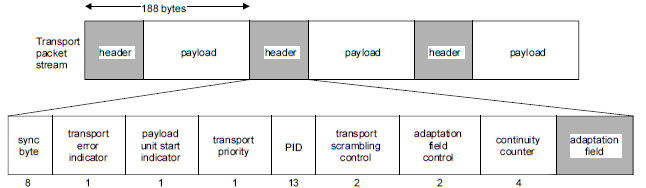
\includegraphics[width=1\linewidth]{figuras/TS_iso13818.png}
\\Source: \citeonline[F.0.1]{ISO}.
\label{fig:TS_iso13818}
\end{figure}

\begin{table}[!h]
\caption{Adaptation Field control values.}
\begin{center}
\begin{tabular}{|c|c|}
\hline
Value & Description \\
\hline
00 & Reserved for future use\\
\hline
01 & No adaptation\hspace{0.1mm}\_\hspace{0.1mm}field, payload only\\
\hline
10 & Adaptation\hspace{0.1mm}\_\hspace{0.1mm}field only, no payload\\
\hline
11 & Adaptation\hspace{0.1mm}\_\hspace{0.1mm}field followed by payload\\
\hline
\end{tabular}
\label{tab_adapataion_field}
\\Source: \citeonline[2.4.3.3]{ISO}
\end{center}
\end{table}

\section{Adaptation Field}

The Adaptation Field (AF) is an optional extension of the TS packet header. Although optional, it contains many useful information and is widely used in practical implementations to carry timing information and to fill with stuffing bytes remaining space in TS packets. \autoref{fig:AdapField_iso13818} shows the concatenation of fields in the Adaptation Field graphically. One characteristic of this extension is that many fields are optional, hence there are several flags that toggle the existence of the fields.

The \textit{adaptation\hspace{0.1mm}\_\hspace{0.1mm}field\hspace{0.1mm}\_\hspace{0.1mm}length} field has 8 bits and specifies the number of bytes in the adaptation field immediately after itself. When there is payload data sharing the TS packet with the adaptation field, this value shall be in the range 0 to 182. If there is no payload, just the AF, the length must be set to 183. For TS packets carrying PES data, stuffing is usually needed in the last TS packet used because PES packets are not necessarily multiples of 188 bytes. Stuffing is accomplished by setting the adaptation field length to more than the sum of the lengths of the data elements in it, so that the remaining payload bytes in PES data exactly fits in the left space. The extra space in the adaptation field is filled with stuffing bytes with the value \texttt{0xFF}.

%This is the only method of stuffing allowed for packets carrying PES data, but for PSI sections another method will be described later.

The \textit{PCR\hspace{0.1mm}\_\hspace{0.1mm}flag} informs the presence of the optional PCR timing information in the \textit{program\hspace{0.1mm}\_\hspace{0.1mm}clock\hspace{0.1mm}\_\hspace{0.1mm}reference\hspace{0.1mm}\_\hspace{0.1mm}base} and \textit{program\hspace{0.1mm}\_\hspace{0.1mm}clock\hspace{0.1mm}\_\hspace{0.1mm}reference\hspace{0.1mm}\_\hspace{0.1mm}extension} fields, that are described in \autoref{Timing}. These fields are wrapped together in \autoref{fig:AdapField_iso13818} as 'PCR', with 42 bits.The other fields will not be described because they are not crucial for the functioning of the multiplexer. However, they are part of the standard and are defined in \citeonline[2.4.3.5]{ISO}.

\begin{figure}
\centering
\caption{Graphical representation of the Adaptation Field.}
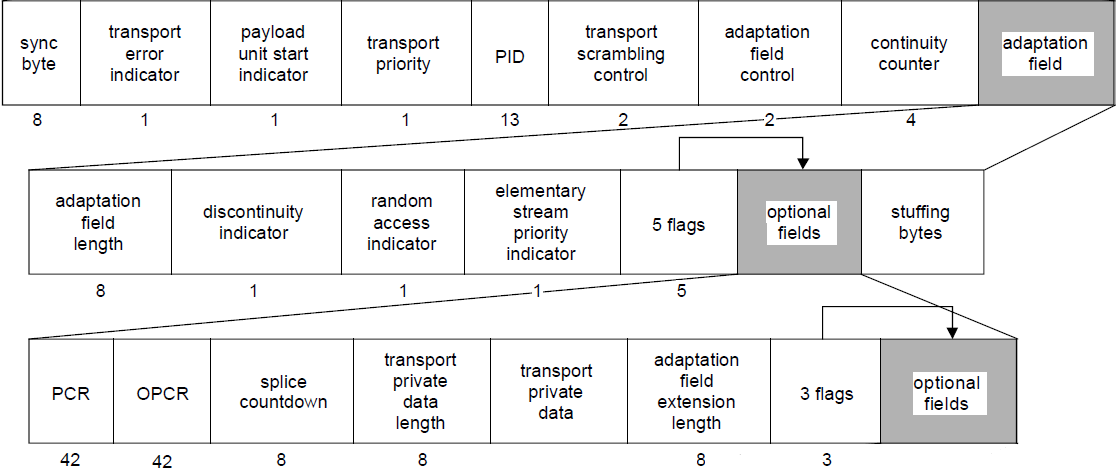
\includegraphics[width=1\linewidth]{figuras/AdapField_iso13818.png}
\\Source and Copyright: \citeonline[F.0.1]{ISO}.
\label{fig:AdapField_iso13818}
\end{figure}

%Na presente seção é descrito o Transport Stream do MPEG2 com suas tabelas PSI. A seguir, na figura \ref{fig:TS_iso13818}, retirada da norma ISO13818 tal qual, é apresentado um esquema da construção de um pacote do TS. Da figura, vê-se que um pacote de TS é formado por 188 bytes de dados. O cabeçalho obrigatório tem 4 bytes, e vai até o campo \textit{continuity counter}. Os dados do pacote podem ainda incluir o \textit{Adaptation Field}, espécie de extensão do cabeçalho, e com informções adicionais para a decodificação do TS. Os fluxos elementares de mídia, os ES, são divididos em pacotes de comprimento variável e formam um PES. Um pacote de TS deve conter o cabeçalho obrigatório com 4 bytes, e a ele devem suceder 184 bytes de dados. Esses bytes restantes podem ser preenchidos de diferentes maneiras:

%\begin{itemize}
%\item{ somente com o \textit{Adaptation Field};}
%\item{ ou com este e mais dados de pacotes PES , que são os fluxos elementares de mídia separados em pacotes;}
%\item{ou ainda com sessões de tabelas de dados complementares aos fluxos, fundamentais para a parametrização do decodificador.}
%\end{itemize}

The ISO13818 standard recommends the TS bit-rate to be constant, according to \citeonline[2.4.2.2]{ISO}. However, to increase the performance of the codecs, their output is necessarily variable, and therefore stuffing bits must be added to the transport streams whenever there is no useful information to be transmitted. To better understand this, take the video encoder as an example: consider that the frame rate is constant and equal to 29.97 frames per second. Since the frames are coded according to the H.264 standard with motion compensation and prediction techniques, the I-frames have necessarily more information than P-frames or even more than B-frames. Therefore, during the transmission of an I-frame, the amount of useful information in the output stream is higher than if a B-frame is being processed. It is up to the multiplexer to handle this variable to constant transformation by filling streams with stuffing bytes.
% ---

\section{Packetized Elementary Stream Header}

The Elementary Streams, when packetized, also receive a header with Systems Layer information. \autoref{fig:PES_iso13818} shows graphically the fields that form the PES Header, and the most significant ones are described in the following list:
\begin{itemize}
\item{The \textit{packet\hspace{0.1mm}\_\hspace{0.1mm}start\hspace{0.1mm}\_\hspace{0.1mm}code\hspace{0.1mm}\_\hspace{0.1mm}prefix} field has 24 bits and constitutes an identification of the start of a packet. Its value is fixed in \texttt{0x000001};}
\item{The \textit{stream\hspace{0.1mm}\_\hspace{0.1mm}ID} is a 8-bit field that may be set to a valid value among those in \autoref{tab_ISOESTypes};}
\item{The \textit{PES\hspace{0.1mm}\_\hspace{0.1mm}packet\hspace{0.1mm}\_\hspace{0.1mm}length} has 16 bits and informs the length of the PES packet from the first bit after the field itself until the end of the packet;}
\item{Among the \textit{7 flags} field in the second row of \autoref{fig:PES_iso13818} is the \textit{PTS\hspace{0.1mm}\_\hspace{0.1mm}DTS\hspace{0.1mm}\_\hspace{0.1mm}flags}, a 2-bit field which informs whether time stamps are present for this packet, and whose values are coded according to \autoref{tab_PTS_DTS_flags}. Time stamps are discussed in \autoref{PTS_DTS}. These time stamps are carried in the \textit{PTS} and/or \textit{DTS} 33-bit fields, shown in the third row of \autoref{fig:PES_iso13818}.}
\end{itemize}

Most of the other fields are intended to carry information to help stream decoding, and are out of the scope of this project.

\begin{table}[!hb]
\caption{PTS\hspace{0.1mm}\_\hspace{0.1mm}DTS\hspace{0.1mm}\_\hspace{0.1mm}flags values.}
\begin{center}
\begin{tabular}{|c|c|}
\hline
Value & Timestamp \\
& Presence \\
\hline
00 & PTS not present; DTS not present\\
\hline
01 & Forbidden\\
\hline
10 & PTS present; DTS not present\\
\hline
11 & PTS present; DTS present\\
\hline
\end{tabular}
\label{tab_PTS_DTS_flags}
\\Source: \citeonline[2.4.3.7]{ISO}
\end{center}
\end{table}

\begin{figure}
\centering
\caption{Graphical representation of the PES Header.}
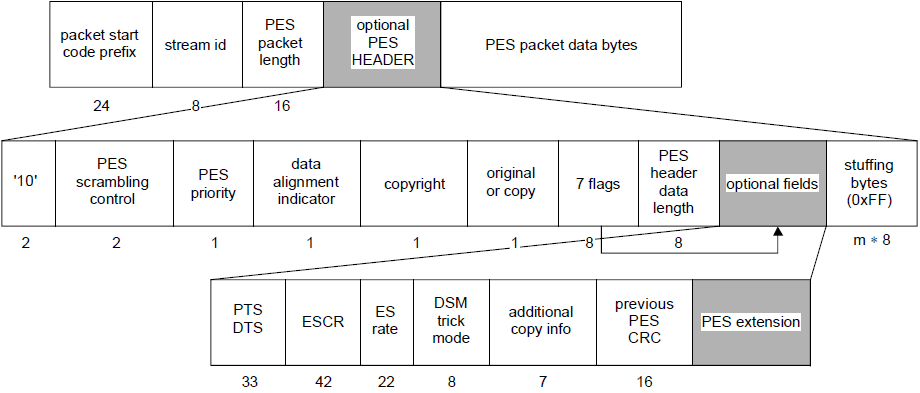
\includegraphics[width=1\linewidth]{figuras/PES_iso13818.png}
\\Source and Copyright: \citeonline[F.0.2]{ISO}.
\label{fig:PES_iso13818}
\end{figure}

\section{Timing}
\label{Timing}

Video and audio information are carried in separate streams that need to be reproduced simultaneously in the receiver, so timing control is crucial to the operation of a television broadcasting system.

The timing model introduced by the standard supposes a constant end-to-end delay from the encoder input, through the transmitter, the receiver and up to the decoder output for all elementary streams of the same program. This way it is possible to theoretically ensure the synchronous playback of both video and audio streams.

The key concept introduced in the ISO standard is the System Time Clock (STC), a reference time base for all the streams in a service being transmitted. The transmitter controls this clock reference for encoding processes and labels each presentation unit with time stamps. The reference clock is sent through the transmission channel and is used by the receiver to lock its own clock to the reference. The media presentation units are transmitted with the time stamps, which are used by the receiver to decode and present the frames at the appropriate time.

If the frequency of the receiver is the same of the transmitter, the encoding, decoding and presentation rates will be the same and the system will work indefinitely as long as there is data to be transmitted. On the other hand, if frequencies are not locked to each other, an inevitable situation of underflow or overflow of the decoder buffers will eventually happen. If an overflow happens, frames will be discarded and not presented. In case of video, if discarded frames would be used to decode other frames, the whole group of pictures is lost. If an underflow happens, there will be freezes in video or mute moments in audio.

It is therefore important to ensure the reconstruction of the STC in the receiver, because the constant delay model is constructed supposing that both sides are perfectly in sync and sets decoding and presentation time stamps to follow the STC. To keep the receiver locked to the reference clock, a digital phase locked loop block is necessary. The following paragraphs describe in greater detail the creation of PCR, PTS and DTS.

%O sincronismo é fundamental para o funcionamento de um sistema de transmissão de televisão, pois é preciso garantir a reprodução do vídeo e do áudio simultaneamente e com a mesma referência temporal. Para possibilitar tal sincronismo, um complexo sistema de sincronismo existe no padrão. O conceito fundamental é a transmissão de um sinal de clock codificado nos pacotes do TS, o PCR, explicado a seguir. Esse sinal é decodificado e alimenta um sistema PLL no decodificador, para então ser utilizado nos fluxos de áudio e vídeo. Os fluxos elementares, por sua vez, transportam referências temporais ao PCR nos campos PTS e DTS, explicados a seguir, e assim são reproduzidos com base em uma mesma referência temporal.

\subsection{PCR}

The STC is implemented as a counter with 42 bits incremented at a 27MHz rate. The reference to this oscillator should be considered to be a GPS satellite signal or an atomic clock oscillator, because the frequency deviation may not be above 810 Hz, with a drift smaller than $ 75 * 10^{-3} $ Hz/s. The STC value is sampled at most every 100ms \citeonline[D.0.3]{ISO} and is encoded in two Program Clock Reference fields (PCR), one in terms of units of 90 KHz and the other in parts of 27MHz. The PCR fields are carried by the Transport Stream inside the TS adaptation field, and might be placed along with Elementary Streams or in individual PIDs. These requirements are defined by \citeonline[2.4]{ISO}.

In the decoder, a digital PLL (Phase Locked Loop) synchronizes the local time reference to the one in the encoder side. The digital PLL is composed by a voltage controlled oscillator(VCO), a counter, a subtractor and a gain adjustment block, as can be seen in \autoref{fig:pll_decoder}. At decoder start-up, the VCO is locally set to oscillate at 27MHz and its signal is used as clock to the counter. Once the first PCR arrives from the received TS, the subtractor outputs the difference between the local PCR and the one sent by the encoder. The result is used as feedback to the VCO, after proper gain adjustment, to sync the local frequency with the encoder. By using this method, the decoder does not need to have an accurate, expensive oscillator, as does the encoder.

The PCR value is not an absolute time reference, but rather the STC starts its counter when the encoding system is turned on. The relationship between the time elapsed since system start-up, $t(i)$, and the PCR value, $PCR(i)$ is calculated as follows, in \autoref{eq:pcr1}. According to \citeonline[2.4.3.5]{ISO} the PCR is carried in two fields within the TS header. The fields names are program\hspace{0.1mm}\_\hspace{0.1mm}clock\hspace{0.1mm}\_\hspace{0.1mm}reference\hspace{0.1mm}\_\hspace{0.1mm}base and program\hspace{0.1mm}\_\hspace{0.1mm}clock\hspace{0.1mm}\_\hspace{0.1mm}reference\hspace{0.1mm}\_\hspace{0.1mm}extension The first part, program\hspace{0.1mm}\_\hspace{0.1mm}clock\hspace{0.1mm}\_\hspace{0.1mm}reference\hspace{0.1mm}\_\hspace{0.1mm}base, is a 33-bit field whose value is given by PCR\hspace{0.1mm}\_\hspace{0.1mm}base(i), as given in \autoref{eq:pcr2}. The second part, program\hspace{0.1mm}\_\hspace{0.1mm}clock\hspace{0.1mm}\_\hspace{0.1mm}reference\hspace{0.1mm}\_\hspace{0.1mm}extension, is a 9-bit field whose value is given by PCR\hspace{0.1mm}\_\hspace{0.1mm}ext(i), as given in \autoref{eq:pcr3}. Yet, as states the standard, \quotation{\textit{the encoded PCR indicates the intended time of arrival of the byte containing the last bit of the program\hspace{0.1mm}\_\hspace{0.1mm}clock\hspace{0.1mm}\_\hspace{0.1mm}reference\hspace{0.1mm}\_\hspace{0.1mm}base at the input of the system target decoder.}}

\begin{equation}
PCR(i) = PCR\hspace{0.1mm}\_\hspace{0.1mm}base(i) * 300 + PCR\hspace{0.1mm}\_\hspace{0.1mm}ext(i)\\
\label{eq:pcr1}
\end{equation}
\begin{equation}
PCR\hspace{0.1mm}\_\hspace{0.1mm}base(i) = ((system\hspace{0.1mm}\_\hspace{0.1mm}clock\hspace{0.1mm}\_\hspace{0.1mm}frequency * t(i)) DIV 300) \% 2^{33}\\
\label{eq:pcr2}
\end{equation}
\begin{equation}
PCR\hspace{0.1mm}\_\hspace{0.1mm}ext(i) = ((system\hspace{0.1mm}\_\hspace{0.1mm}clock\hspace{0.1mm}\_\hspace{0.1mm}frequency * t(i)) DIV 1) \% 300
\label{eq:pcr3}
\end{equation}

% \begin{figure}[!hb]
% \centering
% \caption{PCR Sampling block diagram.}
% 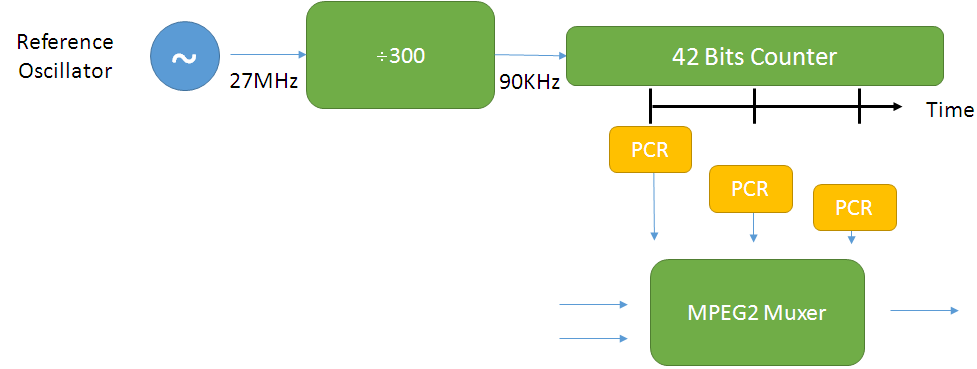
\includegraphics[width=1\linewidth]{figuras/pcr_sampling.png}
% \\Source: The Author.
% \label{fig:pcr_sampling}
% \end{figure}

\begin{figure}[!hb]
\centering
\caption{Decoder PLL block diagram.}
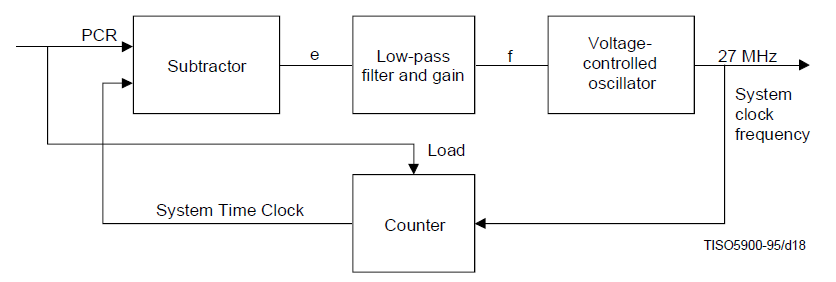
\includegraphics[width=1\linewidth]{figuras/pll_decoder.png}
\\Source and Copyright: \cite{ISO}
\label{fig:pll_decoder}
\end{figure}

Since transmission channels are not perfect, PCR arrival period may vary from one packet to the next, thus subjecting the PCR to jitter. Jitter occurs because packets may arrive out of order or be lost due to transmission errors. In this situation, a discrepancy between the time of arrival of a given PCR and the time that it represents causes the receiver to lose sync with the transmitter.

\autoref{fig:jitter} shows the consequence in the decoder frequency due to jitter in PCR values. PCR TX represents the times that the PCR values are transmitted. PCR RX represent the instants that PCR values are received. STC RX shows the regenerated clock in the receiver. The values \texttt{0} and \texttt{1} are sent and received in schedule and a constant delay of half a period can be identified. PCR value \texttt{2} is sent at $t_a$ but instead of arriving at $t_b$, when it was expected, it arrives at $t_b + \Delta_b$. The receiver STC was in sync with the transmitter and generated value 2 at $t_b$, but since no PCR was received until $t_b + \Delta_b$, a positive error of $\Delta_b$ was calculated and interpreted as if the recevier frequency was too high, i.e., the receiver reached PCR value 2 before the transmitter did. Therefore, the frequency is reduced.

Meanwhile, the transmitter sends PCR value 3 at $t_c$, the packet suffers no jitter and arrives at $t_d$ to the receiver. However, due to the recalculated PLL frequency, the receiver STC will only reach PCR value 3 at $t_d + \Delta_d$, thus creating a negative error value at the subtractor. A negative error value indicates that the internal receiver frequency is lower than necessary and the frequency is increased again. By the time that PCR value 4 reaches the receiver, it is already back in sync and no error is generated.

These oscillations of frequency can be hazardous to program playout, because the receiver buffers are not infinite and a big variation of frequency may lead to buffer overflow or underflow. The consequences of these two situations have already been pointed, they are the loss of groups of pictures or freezes in reproduction.

\begin{figure}[!hb]
\centering
\caption{Jitter consequence in decoder PLL.}
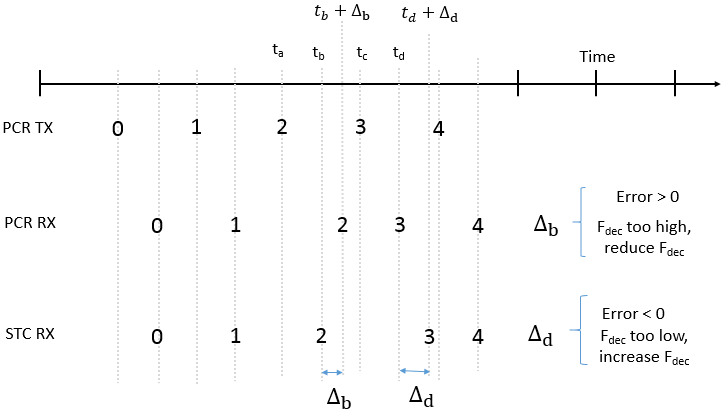
\includegraphics[width=0.8\linewidth]{figuras/jitter.png}
\\Source and Copyright: The author.
\label{fig:jitter}
\end{figure}

\subsection{PTS / DTS}
\label{PTS_DTS}

During the encoding process, video and audio frames are labelled with Presentation and Decoding Time Stamps (PTS and DTS, respectively). The PTS carries the time that the video and audio access units should be displayed in the decoder output. The DTS determines when the frame should be decoded. As was already explained, video encoders with inter-frame prediction reorder frames during encoding process to reduce the amount of transmitted data. In the decoder, frames may arrive out of presentation order and the decoder uses them to resync frame sequence and ensure the expected presentation frame rate. PTS and DTS are generated in a counter driven by a 90KHz clock, obtained by dividing the 27MHz STC signal.

Take \autoref{fig:dts_pts} as an example: the upper row shows frames as they are encoded and transmitted; the middle row, as they are decoded; and the lower row shows the presentation order. The I frame receives DTS value 'N' and PTS 'N+1', since the frame must be decoded completely before presentation. The next frames in the presentation order are $B_1$ and $B_2$ frames, hence they receive PTS 'N+2' and 'N+3', but they can only be decoded after $P_1$ frame has already been decoded, so this $P_1$ frame gets DTS 'N+1' and the B frames would get DTSs 'N+2' and 'N+3'. According to the standard, if the PTS is equal to the DTS, there is no need to send both time stamps and B frames only have PTS. The $P_1$ frame should be presented after the two B frames, so it gets PTS 'N+4'. The process continues for the next B- and P-frames. The PTS field calculation follows what stated in \autoref{eq:pts}: the k-th PTS field for a given stream corresponds to the presentation time $t_p(k)$. The decoder displays frames in the output buffer when its presentation counter reaches $PTS(k)$. The calculation of DTSs follows exactly the same equation.

\begin{figure}[!hb]
\centering
\caption{Example of PTS and DTS use.}
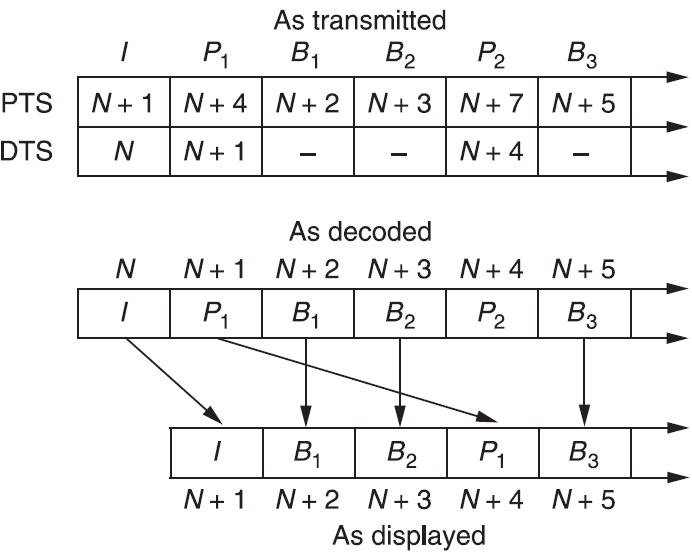
\includegraphics[width=0.5\linewidth]{figuras/dts_pts_2.png}
\\Source and Copyright: \cite{watkinson}
\label{fig:dts_pts}
\end{figure}

\begin{equation}
PTS(k) = ((system\hspace{0.1mm}\_\hspace{0.1mm}clock\hspace{0.1mm}\_\hspace{0.1mm}frequency * t_p(k)) DIV 300) \% 2^{33}\\
\label{eq:pts}
\end{equation}

%\subsection{PTS / DTS}

%Os campos Decoding Time Stamp \(DTS\) e Presentation Time Stamp \(PTS\) são outros dois referenciais de tempo, derivados do PCR, e que servem a informar ao decodificador o instante de tempo em que devem ser decodificadas e exibidas, respectivamente, as Access Units de vídeo e áudio. Uma Presentation Unit \(PU\) é definida pela norma como sendo um quadro de áudio ou de vídeo, e uma Access Unit \(AU\) é a representação codificada da Presentation Unit.

%A norma define claramente qual instante de tempo deve ser considerado para gerar o PTS ou o DTS: \quotation{No caso do áudio, se um PTS está presente num cabeçalho de PES, este deve fazer referência à primeira AU que comece no pacote. Uma AU de áudio começa em um pacote se o primeiro byte da AU de áudio estiver presente no pacote. No caso do vídeo, se um PTS está presente no cabeçalho do pacote PES, este deve se referir à AU que cujo primeiro \textit{start\hspace{0.1mm}\_\hspace{0.1mm}code} está neste pacote.}

% ---

\section{Program Specific Information}
\label{iso_psi}

Program Specific Information(PSI) is a set of normative data useful to transmission, demultiplexing and presentation of audio, video and data streams. The PSI set is organized in tables, each with a specific function in the standard. The tables that carry information about which PIDs carry video and audio streams, called PAT (Program Association Table) and PMT (Program Map Table) are mandatory and their syntax is defined by the ISO/IEC13818-1 standard. The Network Information Table is also mandatory according to the standard, but its syntax is not defined by ISO/IEC. There is another set of tables that are not mandatory according to ISO13818, but ABNT NBR15603 defines as mandatory, as will be seen in \autoref{nbr15603}.

Since programs may change of structure during transmission, for example a movie with multiple audio streams starts playout right after the local news with a single audio stream, PSI tables must follow this change too. To inform the decoder whether a table been transmitted is valid at the moment or not, there are two fields in each section of the tables, the \textit{version\hspace{0.1mm}\_\hspace{0.1mm}number} and the \textit{current\hspace{0.1mm}\_\hspace{0.1mm}next\hspace{0.1mm}\_\hspace{0.1mm}indicator}.

The Conditional Access Table must be present only if scrambling is employed. The Network Information Table is optional and its contents are not specified by ISO/IEC13818-1. The NIT used in SBTVD is defined by ABNT NBR15603.

The ISO standard defines that the PSI tables must be sent in sections and that the sections can be segmented to fit the TS packets. Sections can not be longer than 1024 bytes, although in practice the number of bytes for the mandatory tables is very below that. There are several common fields to all PSI tables, they may vary of value but their syntax is the same:
\begin{itemize}
\item{The field \textit{table\hspace{0.1mm}\_\hspace{0.1mm}ID} has 8 bits and defines what is the table's type, according to \autoref{fig:tab_psi_tables_ids};}
\item{The field \textit{section\hspace{0.1mm}\_\hspace{0.1mm}syntax\hspace{0.1mm}\_\hspace{0.1mm}indicator} is a 1-bit field which shall always be set to '1';}
\item{The field \textit{section\hspace{0.1mm}\_\hspace{0.1mm}length} has 12 bits, the first most significant two shall be '00' and the other 10 bits are the length of the section, starting at the first bit after the length field and including the CRC;}
\item{The field \textit{version\hspace{0.1mm}\_\hspace{0.1mm}number} has 5 bits, and should be incremented by one every time any information in the respective table changes;}
\item{The field \textit{current\hspace{0.1mm}\_\hspace{0.1mm}next\hspace{0.1mm}\_\hspace{0.1mm}indicator} has 1 bit, and identifies whether the respective table is valid at the moment of transmission or will be valid later;}
\item{The field \textit{section\hspace{0.1mm}\_\hspace{0.1mm}number} has 8 bits, and is used to order long, multiple section, tables. In practice, tables usually fit in a single section and this value is set to \texttt{0x00}}
\item{The field \textit{last\hspace{0.1mm}\_\hspace{0.1mm}section\hspace{0.1mm}\_\hspace{0.1mm}number} has 8 bits, and is used to inform which was the \textit{section\hspace{0.1mm}\_\hspace{0.1mm}number} of the previous transmitted section. In practice, since tables only fill one section, this field is set to \texttt{0x00}, too.}
\end{itemize}


Descriptors are structures used to extend the definitions of services and their elements. All descriptors have the same format: they begin with an 8-bit tag value, then there is an 8-bit length field and variable length data bytes. The standard defines a considerable amount of descriptors, but not all of them are used in practical applications. A selection of the descriptors used in the project are presented in \autoref{descriptors}.

%O PSI é o conjunto de informações especificas ao programa, ou \textit{Program Specific information}, em inglês, e serve para organizar as informações de transmissão, sincronismo, decodificação e apresentação dos fluxos de áudio, vídeo e dados. O PSI é organizado em forma de tabelas, cada uma com uma função específica no padrão. As tabelas que servem a indicar ao decodificador onde estão no TS os fluxos de vídeo e áudio, chamadas de PAT( Tabela de associação de programas) e PMT (Tabela de Mapeamento de Programas), são obrigatórias, Há ainda um conjunto grande de tabelas que servem a outros fins, e que não são obrigatórias segundo a ISO13818, mas que a ABNT NBR15603 define como obrigatórias.
%A norma ISO define que as tabelas do PSI devem ser enviadas em seções e as seções podem ser segmentadas para caberem nos pacotes de TS. As seções não podem ter mais de 1024 bytes, embora na prática o número de bytes para uma tabela obrigatória fique bem abaixo. A sintaxe das tabelas é padronizada. Um campo no início da tabela (table\hspace{0.1mm}\_\hspace{0.1mm}ID) define qual o seu tipo (PAT,PMT, etc.) e o campo section number serve como um contador caso a tabela seja dividida em diversas seções. O campo version umos campos que seguem são personalizados version, section number, program number.

\subsection{Program Association Table}

The Program Association Table (PAT) indicates the PID of the corresponding Program Map Table (PMT) for each service in the multiplexer. It lists, for every program on the stream, its unique \textit{program number} and the PID of that program's PMT, the \textit{program map PID}. The PAT is assigned to the fixed PID \texttt{0x0000}, so the decoder can always know where to look for first and then find the PMT of each service in the PIDs pointed by the PAT. The field \textit{table\hspace{0.1mm}\_\hspace{0.1mm}ID} is always \texttt{0x00} for PAT. The field \textit{transport\hspace{0.1mm}\_\hspace{0.1mm}stream\hspace{0.1mm}\_\hspace{0.1mm}ID} has 16 bits and represents a unique ID to differentiate this Transport Stream from all streams in a network. In SBTVD, this value is calculated based on geographic position of the transmitter and the broadcaster's call signs \footnote{A call sign is a unique designation for a transmitting station. In Brazil, the range assigned by ITU for broadcast stations is from ZVA-000 to ZZZ999.}. Additionally to the common fields, this table also carry the following fields, in a loop, right after \textit{last\hspace{0.1mm}\_\hspace{0.1mm}section\hspace{0.1mm}\_\hspace{0.1mm}number}:

\begin{itemize}
\item{first a \textit{program\hspace{0.1mm}\_\hspace{0.1mm}number} field, with 16 bits, names the first program in the TS;}
\item{ then a 13-bit field, \textit{program\hspace{0.1mm}\_\hspace{0.1mm}map\hspace{0.1mm}\_\hspace{0.1mm}PID} points the PID value of the corresponding PMT;}
\item{if the \textit{program\hspace{0.1mm}\_\hspace{0.1mm}number} is \texttt{0x00}, instead of the above definition, ISO specifies that the PID pointed to is the one of the NIT, and the field is called \textit{network\hspace{0.1mm}\_\hspace{0.1mm}PID}.}
\end{itemize}

A PAT table section is analysed in \autoref{pat_pmt_analysis}.

\subsection{Program Map Table}
\label{PMT}

One Transport Stream must have as many Program Map Tables as services. Each Program Map Table (PMT) in the TS indicates which PIDs contain the elementary streams corresponding to one service. It links a \textbf{program number} to several \textbf{elementary PIDs}. Each elementary stream must have a \textbf{type} identification, which designate the nature of the stream, according to ISO13818-1, and defines roughly whether it is a video, audio or data stream. \autoref{tab_ISOESTypes} is an excerpt of the standardized types. Apart from the common fields already presented in the introductory chapter, the PMT also has the following fields:

\begin{itemize}
\item{a \textit{program\hspace{0.1mm}\_\hspace{0.1mm}number} field, with 16 bits, designates the program specified by this section;}
\item{then a 13-bit field, the \textit{PCR\hspace{0.1mm}\_\hspace{0.1mm}PID} points the PID whose adaptation field contains the PCR that should be used to sync this service ;}
\item{if the \textit{program\hspace{0.1mm}\_\hspace{0.1mm}number} is \texttt{0x00}, instead of the above definition, ISO specifies that the PID pointed to is the one of the NIT, and the field is called \textit{network\hspace{0.1mm}\_\hspace{0.1mm}PID}.}
\item{The field \textit{program\hspace{0.1mm}\_\hspace{0.1mm}info\hspace{0.1mm}\_\hspace{0.1mm}length} has 12 bits, the first most significant two shall be '00' and the other 10 bits represent the length of the section descriptors, in bytes;}
\item{the \textit{stream\hspace{0.1mm}\_\hspace{0.1mm}type} field has 8 bits, and as already discussed, should be filled with the standardized designation of a stream according to \autoref{tab_ISOESTypes};}
\item{the \textit{elementary\hspace{0.1mm}\_\hspace{0.1mm}PID} field has 13 bits and make reference to the PID with the stream whose type is in \textit{stream\hspace{0.1mm}\_\hspace{0.1mm}type};}
\item{the \textit{ES\hspace{0.1mm}\_\hspace{0.1mm}info\hspace{0.1mm}\_\hspace{0.1mm}length} has 12 bits, the first most significant two shall be '00' and the other 10 bits represent the length of the ES descriptors;}
\item{what follows are a variable number of descriptors, whose syntax will be discussed in \autoref{descriptors}.}
\end{itemize}

A PMT table section is analysed in \autoref{pat_pmt_analysis}.

\subsection{Further Considerations}

Although ISO/IEC13818-1 defines other tables, such as the Conditional Access Table, these are not commonly used in free to air television broadcasting systems and were left off the scope of the project.

\chapter{ABNT NBR15603 Standard}
\label{nbr15603}

\section{Introduction}

The ABNT NBR15603 standard is divided into three parts, each one describes a portion of the SBTVD Systems Layer. Most of the content is an adaptation of the original ISO/IEC13818-1 standard, and there is no reason to be reproduced, but some peculiarities are worth to be detailed. Also, some contents were defined based on the ARIB STD-B10. There is a set of tables not defined in MPEG2 Systems, among them the Network Information Table, that are mandatory in SBTVD. The PIDs that must be used to transmit the Tables are slightly different than what is defined on ISO/IEC13818-1. \autoref{fig:tab_psi_tables_names_pids_abnt} in \autoref{tables_abnt} shows the modified values. \autoref{fig:tab_psi_tables_ids_level_frequency} also in \autoref{tables_abnt} brings other two important information: first, the transmission level of each table, whether its transmission is mandatory( \textit{"obrigatório"} means mandatory) or optional; and the repetition rate of each table in the stream, in units of repetitions per milliseconds. The tables whose transmission is mandatory are Program Association Table (PAT), Program Map Table (PMT), Network Information Table (NIT), Service Description Table (SDT), Time Offset Table (TOT), Event Information Table (EIT) and Conditional Access Table (CAT)(if the transmission is scrambled\footnote{Scrambling methods are used to prevent receptors without permission to open certain streams from viewing them. They are usually used in paid television systems but not in broadcast systems.}). The following is a brief description of the mandatory tables that have not yet been discussed in \autoref{iso13818}.

\section{System Information} 
\label{abnt_psi}

\subsection{Service Description Table (SDT)}
\label{SDT}
The Service Description Table brings useful information to describe the services contained in the TS. Multiple SDTs can be transmitted, corresponding to different Transport Streams, but in practical broadcast implementations this feature is not used. Services information is coded into SDT in a loop. For every service, it carries flags signalling the presence of another mandatory table, the EIT, which is described in \autoref{EIT}, a \textit{running\hspace{0.1mm}\_\hspace{0.1mm}status} flag with 3 bits informs to the decoder if the service is currently running; and other flags as described in \citeonline[7.2.6.1]{NBR}.

\subsection{Network Information Table (NIT)}
\label{NIT}
The Network Information Table carries information about the physical organization of the network, such as the network ID, and all the characteristics about the transmission channel, such as modulation method, frequency and channels. Most of the useful information of the NIT is carried in descriptors, discussed in \autoref{nit_descriptors}. The fields in the NIT section apart from the common fields are the following:
\begin{itemize}
\item{\textit{network\hspace{0.1mm}\_\hspace{0.1mm}ID} field, with 16 bits, contains a unique network identification, calculated as described in \autoref{special_fields};}
\item{\textit{network\hspace{0.1mm}\_\hspace{0.1mm}descriptors\hspace{0.1mm}\_\hspace{0.1mm}length} contains the byte number of all the network descriptors;}
\item{\textit{transport\hspace{0.1mm}\_\hspace{0.1mm}stream\hspace{0.1mm}\_\hspace{0.1mm}loop\hspace{0.1mm}\_\hspace{0.1mm}length} contains the byte number of all the transport stream loop descriptors;}
\item{\textit{transport\hspace{0.1mm}\_\hspace{0.1mm}stream\hspace{0.1mm}\_\hspace{0.1mm}ID} contains the unique TS ID, the same that is in PAT;}
\item{\textit{original\hspace{0.1mm}\_\hspace{0.1mm}network\hspace{0.1mm}\_\hspace{0.1mm}ID}  contains the same value of \textit{network\hspace{0.1mm}\_\hspace{0.1mm}ID} field;}
\item{\textit{transport\hspace{0.1mm}\_\hspace{0.1mm}descriptors\hspace{0.1mm}\_\hspace{0.1mm}length} contains the byte number of all the transport descriptors.}
\end{itemize}

\subsection{Time Offset Table (TOT)}
\label{TOT}
The Time Offset Table contains a \texttt{UTC-3\hspace{0.1mm}\_\hspace{0.1mm}time} field, with 40 bits, to hold the information about the current time and date. The two most significant bytes correspond to the least significant bits of the Modified Julian Date \citeonline[Annex A]{NBR}. The other 3 bytes represent the time of the day with 6 digits in BCD encoding, so that 14:54:22 is encoded as \texttt{0x145422} in hexadecimal.

The only descriptor that the TOT contains is the \textit{local\hspace{0.1mm}\_\hspace{0.1mm}time\hspace{0.1mm}\_\hspace{0.1mm}offset\hspace{0.1mm}\_\hspace{0.1mm}descriptor}. It indicates the time and date when there will be a transition of time, such as Daylight Saving Time periods and must be compliant to the EN 300 468:2007 standard, subsection 5.2.19 \citeonline[8.3.25]{NBR}.

\subsection{Event Information Table (EIT)}
\label{EIT}
The Event Information Table was not yet investigated and is currently not implemented. Although it is mandatory, its absence does not affect the functioning of the system, as will be shown in \autoref{test_remultiplexing}.

\section{Program and System Descriptors}
\label{descriptors}
Descriptors are structures of data with a standardized syntax that increase the flexibility of tables to carry specific information related to the broadcasting system, the streams contents and program guides, for example. Their syntax always starts with a \textit{tag} byte, followed by one \textit{length} byte or two, and end with the descriptor \textit{data} itself. The lengths of data fields are flexible, it depends on the information carried by the descriptor. If it is the descriptor of the name of the broadcaster, then it must be variable, but if it's rather the descriptor carrying the central frequency of the channel, it must have always the same size.

The ABNT standard defines a set of descriptors whose presence is mandatory in each of the mandatory tables. They are all listed because one target of the project is to implement all in the application:

\begin{itemize}

\item in the PAT there are no defined descriptors;
\item in the PMT the following are mandatory: \textit{AAC descriptor} and \textit{Parental rating descriptor}, other descriptors are only mandatory under circumstances \citeonline[8.1]{NBR};
\item in the NIT the following are mandatory: \textit{Network name descriptor}, \textit{Service list descriptor}, \textit{TS information descriptor}, \textit{Terrestrial delivery system descriptor}, \textit{Partial reception descriptor} (for 1-Segment reception) and \textit{System management descriptor};
\item in the SDT the following is mandatory: \textit{Service descriptor};
\item in the TOT the following is mandatory: \textit{Local time offset descriptor};
\item in the EIT the following is mandatory: \textit{Parental rating descriptor}.
\end{itemize}

Each descriptor is briefly described in the following sections.

\subsection{Program Map Table Descriptors}
\label{pmt_descriptors}
The \textit{AAC descriptor} is not defined in the ABNT standard. The ABNT Operational Guideline for SBTVD suggests the following syntax: the first byte is the descriptor tag, with value \texttt{0x7C}; the second byte is the descriptor length, to be filled appropriately; a third byte is to inform the profile and level of the audio streams of the service described by the PMT, whose values are defined in a table\cite{guia} and are \texttt{0x29} for AAC Profile - level 2 or \texttt{0x2E} for HE-AAC Profile - level 4, just to cite two examples. The fourth byte has only a flag to set whether an optional field is used in the following bytes, but it is not used in practical applications.

The \textit{Parental rating descriptor} tag is \texttt{}, after the length byte what follows is a loop of four bytes: the first three represent a country code with three characters encoded according to ISO 8859-15\footnote{ISO 8859 is a character encoding standard similar to the well known ASCII standard, but more complete in terms of characters foreign to the English language. Each character is encoded as a number.}, for Brazil the characters are \texttt{BRA} which are coded as \texttt{0x42 0x52 0x41}. The other byte in the loop is the rating for the service being broadcasted. The first four bits encode the minimum age to watch: from free to all audiences (\texttt{'0001'}) to above 18 years only (\texttt{'0110'}), with steps in 10 years, 12, 14 and 16. The codes outside this range are forbidden. The other four bits inform the presence of scenes with drugs (\texttt{'0001'}), violence (\texttt{'0010'}) and sex (\texttt{'0100'}). Combinations of these values are possible, so if a show has scenes of drugs and violence, the four bits would be \texttt{'0011'}, the most significant bit is reserved for future applications.

\subsection{Network Information Descriptors}
\label{nit_descriptors}
The \textit{Network name descriptor} carries the name of the transmission system. Tag and length have one byte each, and the name is encoded according to the ISO 8859-15 standard in the rest of the descriptor. The network names for two of the local broadcasters in Porto Alegre are "Band HDTV" and "RBS TV POA".

The \textit{Service list descriptor} provides a list of all the services in the Transport Stream. Tag and length have one byte each, and the data fields are formed with a loop of two fields: \texttt{service\hspace{0.1mm}\_\hspace{0.1mm}id} and \texttt{service\hspace{0.1mm}\_\hspace{0.1mm}type}. The service ID is the same as the program number defined in the PMT and explained below. The service type is defined by ABNT \citeonline[8.3.13]{NBR}: \texttt{0x00} for HDTV and SDTV services and \texttt{0xC0} for 1-Segment services.

The \textit{TS information descriptor} carries in the \texttt{remote\hspace{0.1mm}\_\hspace{0.1mm}control\hspace{0.1mm}\_\hspace{0.1mm}key\hspace{0.1mm}\_\hspace{0.1mm}id} field the virtual channel associated to the transport stream. \texttt{ts\hspace{0.1mm}\_\hspace{0.1mm}name\hspace{0.1mm}\_\hspace{0.1mm}char} carries the name of the TS, which is the same as in the \textit{network name descriptor}. The field \texttt{transmission\hspace{0.1mm}\_\hspace{0.1mm}type\hspace{0.1mm}\_\hspace{0.1mm}count} states the number of transmission types in the TS. The field \texttt{transmission\hspace{0.1mm}\_\hspace{0.1mm}type\hspace{0.1mm}\_\hspace{0.1mm}info} is repeated for each type and is used to designate the hierarchical layers and other transmission parameters. The definition of its value was not found in the standard, so an analysis was done in the local broadcasters streams to discover what were used the values. For HD services, the value is \texttt{0x0F} and for 1-Segment it is \texttt{0xAF}. Next, a list of the services that are included in each of the layers is added.

The \textit{Terrestrial delivery system descriptor} indicates several physical conditions of the transmission channel. After tag and length, what follows is an \texttt{area\hspace{0.1mm}\_\hspace{0.1mm}code} field, calculated according to \autoref{special_fields} 

The \textit{Partial reception descriptor} carries the service ID that contains the 1-Segment reception service. It is only mandatory if partial reception is used.

The \textit{System management descriptor} identifies if the Transport Stream contains free to air or paid content, and if the transmission system is the SBTVD or other. Further information is available in the standard \citeonline[8.3.21]{NBR}.

The service ID field has 16 bits. The eleven most significant are the less significant on the network ID. The next two bits are the service type, \texttt{0x00} for television and \texttt{0x11} for 1-Segment television. The last three bits are the service number, a counter representing at most 8 services.

\subsection{Service Description Table Descriptors}
\label{sdt_descriptors}

The \textit{Service descriptor} is the only mandatory descriptor in SDT, and there must be as many of it as services in the TS. It carries the name of the provider and the name of each service in the Transport Stream. After tag and length fields there is a service type field, whose value is the same as defined above in \autoref {nit_descriptors}. What follows is a sequence of bytes encoding each character of the provider name and the service name.

\subsection{Special Fields}
\label{special_fields}

The area code is calculated as follows\citeonline[Annex E]{NBR}. It is formed by 12 bits, the 5 most significant are a unique code per state and the other 7 are an identification of the region according to the IBGE\footnote{IBGE is the Brazilian Institute of Geography and Statistics. It is the agency responsible for statistical, geographic, cartographic, geodetic and environmental information in Brazil.}. Next comes the \texttt{guard\hspace{0.1mm}\_\hspace{0.1mm}interval}, with 2 bits mapping the four possible values for the guard interval: 1/32 is \texttt{0x00}, 1/16 is \texttt{0x01}, 1/8 is \texttt{0x10} and 1/4 is \texttt{0x11}.  Next comes the \texttt{transmission\hspace{0.1mm}\_\hspace{0.1mm}mode}, other two bits mapping the following modes: mode 1 is \texttt{0x00}, mode 2 is \texttt{0x01} and mode 3 is \texttt{0x10}. Finally is added the frequency of the central channel, encoded with the following syntax: $(473 + 6 * (X - 14) + 1/7) * 7 = $ \texttt{frequency} in MHz, where X is the channel number from 14 to 69.

The fields \texttt{network\hspace{0.1mm}\_\hspace{0.1mm}ID}, \texttt{original\hspace{0.1mm}\_\hspace{0.1mm}network\hspace{0.1mm}\_\hspace{0.1mm}ID} and \texttt{service\hspace{0.1mm}\_\hspace{0.1mm}ID} are calculated according to Annex H in \cite{NBR}. To calculate the \texttt {network\hspace{0.1mm}\_\hspace{0.1mm}ID} one should take the call sign of the broadcaster, consider only the last letter and the three digits. To each of the possible letters (A, B, P, Q, T) is associated a number from 0 to 4, in the letter order presented here, which is concatenated to the three digits and form a number in decimal base. This number converted to binary forms the \texttt{network\hspace{0.1mm}\_\hspace{0.1mm}ID}. As an example, the standard cites the call sign "ZYB205. The letters "ZY" are discarded and the "B" becomes a 1. The network ID is 1205, that in hexadecimal base is \texttt{0x04B5}.

% An example of an hypothetical decoder start-up operation is shown in \autoref{fig:funcionamento_inicial_decoder}.

% \begin{figure}[!hb]
% \centering
% \caption{Hypothetical decoder initial operation.}
% 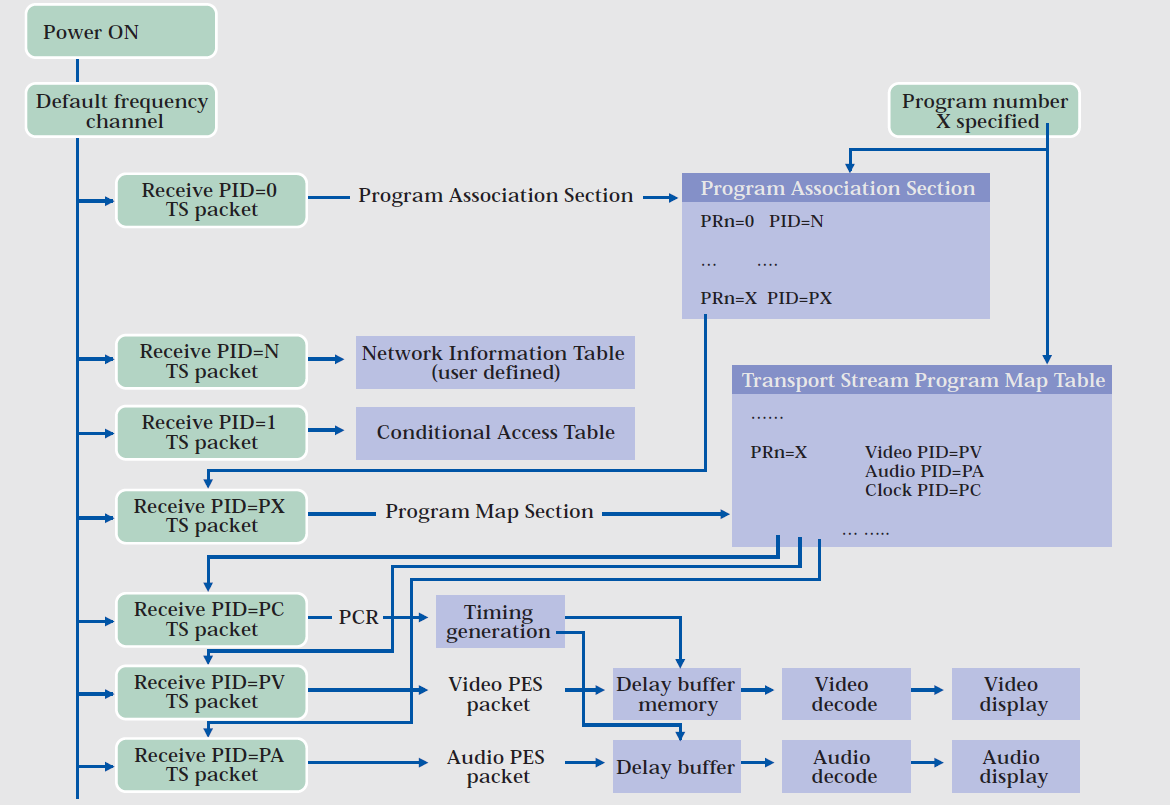
\includegraphics[width=0.8\linewidth]{figuras/funcionamento_inicial_decoder.png}
% \\Source and Copyright: \cite{nhk}.
% \label{fig:funcionamento_inicial_decoder}
% \end{figure}

%\section{Recommendations on the ABNT NBR 15608}

\chapter{Available Solutions and Limitations}

A quick search on a search engine for the keywords \textit{MPEG2 TS multiplexer} returns a long list of commercial solutions for multiplexing media files of most different formats in MPEG2 standard. The commercial solutions are usually associated with dedicated hardware, such as the solution presented by \cite{harris}, which are targeted for broadcasters and are expensive, of the order of a few thousand dollars. The main customers of these solutions are television broadcasters, producing live content and need low latency for signal encoding. These devices operate in real time, receiving streams of video, audio and data across multiple ASI interfaces and delivering output in a multiplexed stream in MPEG2 standard. The free solutions are software compatible with Windows and Linux platforms, mostly. Some have graphics and pattern to aid its use by users unfamiliar with the standard interface configurations. The main difference is that the goal is not the user of the system in real time, so that the specification for the processing and memory of personal computers are usually sufficient to run the tools. The input and output interfaces are commonly files that store binary data streams in a sequential manner.

%Uma busca rápida em um motor de pesquisa pelas palavras-chave \textit{MPEG2 TS muxer} retorna uma infinidade de soluçoes comerciais e gratuitas para a multiplexaçao de arquivos de mídia dos mais diferentes formatos no padrão MPEG2. As soluçoes comerciais geralmente estão associadas a \textit{hardwares} dedicados, como a apresentada por \cite{harris} e custam elevadas somas, da ordem de alguns milhares de dólares. Estes equipamentos funcionam em tempo real, recebendo fluxos de vídeo, áudio e dados em múltiplas interfaces de entrada ASI e entregando na saída um fluxo multiplexado no padrão MPEG2. Os principais clientes destas soluções são geradoras de televisão, que produzem conteúdo ao vivo e precisam de baixa latência na codificação do sinal. As soluções gratuitas são \textit{softwares} compatíveis com as plataformas Windows e Linux, na sua maioria. Alguns têm interface gráfica e configuraçoes padrão para auxiliar o seu uso por usuários pouco familiarizados com o padrão. A principal diferença é que o objetivo não é a utilizaçao do sistema em tempo real, de modo que as especificaçoes de processamento e memória dos computadores pessoais geralmente são suficientes para executar as ferramentas. As interfaces de entrada e saída são comumente arquivos binários que armazenam os fluxos de dados de maneira sequencial.

%Para fins de elaboraçao da ferramenta de multiplexação proposta neste trabalho, algumas ferramentas gratuitas foram escolhidas para estudo. Para a escolha destas ferramentas em particular, os critérios foram os seguintes:
%\begin{itemize}
%\item{as ferramentas deveriam ser de código aberto e com licença freeware, para manter os aspectos legais no projeto;}
%\item{as ferramentas deveriam possibilitar a modificaçao do código para adaptar-se o máximo possivel a situaçao atual de cada programa à norma brasileira;}
%\item{o desenvolvimento das ferramentas deveria estar ativo, ou seja, não se considerou soluções antigas, que não tenham sofrido atualizaçoes nos últimos 5 anos;}
%\item{as ferramentas precisam apresentar compatibilidade nativa com os fluxos elementares padrão da norma brasileira, como as codificações de vídeo H.264 e áudio AAC empacotado por LATM.}
%\end{itemize}

In order to develop the multiplexing tool proposed in the project, some open-source tools were picked to be studied. The criteria for choosing the solutions were the following:
\begin{itemize}
\item{the application should be freeware and the source code should be under open-source licences;}
\item{the organization of the source code should facilitate its modification to add new features and data;}
\item{the tool should be under current development, solutions without updates in the last 5 years were not considered;}
\item{the tool must contain native compatibility with the elementary streams defined in the SBTVD standard, such as H.264 video and AAC/LATM audio.}
\end{itemize}

A brief description of the solutions that met most of these requirements is presented in the following paragraphs. After that, a tables synthesizes the key features of the two best of them.

%As soluções encontradas que atendem a essas condiçoes são apresentadas na sequência, com detalhes das características individuais.

%==> julgou-se inicialmente que ela deveria ser desenvolvida desde o início, mas após a pesquisa 

%Multiplos Serviços(program number)
%Encoder Fluxos Video e Audio(h264, aac-latm)
%Garantia de Sincronismo (calculo do PTS/PCR)
%Criaçao de Fluxo TS com taxa de bits constante


\section{FFMPEG}
%Segundo os próprios desenvolvedores, o FFMPEG é uma ferramenta versátil de codificaçao, decodificação, verificaçao e exibiçao de fluxos de vídeo, áudio e legendas. Com um conjunto vasto de bibliotecas de código aberto, permite conversão entre diferentes formatos, taxa de quadros, tamanho de quadro de vídeo, amostragem de áudio, dentre outras funçoes. É a solução mais completa e em mais expressivo desenvolvimento, com atualizações diárias organizadas em um repositório público. Nativamente, não permite a criaçao de fluxos TS com múltiplos serviços(ou programas). É capaz de entregar na saída vídeos codificados em formato H.264 e áudios AAC-LATM. É possível manter o sincronismo entre os fluxos, quer mantendo as informaçoes presentes nos fluxos originais, quer gerando novas marcações temporais. Se desejado, uma taxa constante de bits pode ser programada e o resultado é confiável.
%Segundo os próprios desenvolvedores, o FFMPEG é uma ferramenta versátil de codificaçao, decodificação, verificaçao e exibiçao de fluxos de vídeo, áudio e legendas. Com um conjunto vasto de bibliotecas de código aberto, permite conversão entre diferentes formatos, taxa de quadros, tamanho de quadro de vídeo, amostragem de áudio, dentre outras funçoes. É a solução mais completa e em mais expressivo desenvolvimento, com atualizações diárias organizadas em um repositório público. Nativamente, não permite a criaçao de fluxos TS com múltiplos serviços(ou programas). É capaz de entregar na saída vídeos codificados em formato H.264 e áudios AAC-LATM. É possível manter o sincronismo entre os fluxos, quer mantendo as informaçoes presentes nos fluxos originais, quer gerando novas marcações temporais. Se desejado, uma taxa constante de bits pode ser programada e o resultado é confiável.

According to the developers themselves, FFmpeg is a versatile tool for encoding, decoding, verifying and displaying video, audio and subtitle streams. With a broad set of open source libraries, allows conversion between different formats, frame rate, video frame size, audio sample rate, among other functions. It is the most complete and under most significant development, with daily updates organized in a public repository.
Natively, it does not allow the creation of TS streams with multiple services (or programs). It is capable of delivering the output videos encoded in H.264 and AAC-LATM audio. It maintains synchronization between flows, either by keeping the timing information present in the original flows or generating new temporal tags. If desired, a constant TS bit rate can be set and the result is reliable.


\section{GPAC}
%Ferramenta desenvolvida pela Escola Francesa Télécom ParisTech, apresenta características similares à anterior, mas é menos performante no que compete ao sincronismo e à manutenção de uma taxa constante de bits no arquivo de saída. Suporta a criação de múltiplos serviços, mas apresenta comportamento aleatório no número de pacotes gerados. Observou-se diversas vezes que, para arquivos de entrada com 10 segundos de duraçao e as mesmas configurações da ferramenta, eventualmente eram gerados desde 7 segundos até 15 segundos, o que sugere uma falta de controle do sistema. Consequentemente, quando o arquivo era gerado com tempo diferente do original, a taxa de reprodução dos fluxos ficava alterada e o resultado não era aproveitável para exibição.

The GPAC tool was developed by the French school Télécom ParisTech, that has similar characteristics to FFmpeg, but is less performing in keeping timing accurate and maintaining a constant bit rate of the output file. Supports the creation of multiple services, but demonstrated a random behavior in the number of packets generated for the same input files and parameters. For example, for the same input files with 10 seconds of duration and same input settings, the tool was tested ten times and generated from 7 to 15 seconds of TS output on the ten trials, which suggests a lack of bit rate control.

\begin{table}[!htpd]
\caption{Comparison of the Available Solutions}
\begin{center}
\begin{tabular}{|c|c|c|c|}
\hline
Tool & Multi-service & LATM & Sync\\
\hline
FFmpeg & NO & YES & YES\\
\hline
GPAC & YES & NO & NO\\
\hline
\end{tabular}
\label{tab_comparison_tools}
\\Source: Tests made by the author.
\end{center}
\end{table}

\section{Available Solutions Choice}

Even though FFMPEG doesn't provide native support for multiple MPEG services, it was chosen as the base solution to the project because it was noticed that the modifications to the source code in order to add this feature were likely to be implemented in the available time. The existing timing feature counted towards this option, too. FFMPEG has a public API that could have been used to develop a multiplexing application from scratch, but a modification of the existing structure seemed more rational considering the existing object-oriented architecture and the available development time. Most of the MPEG2 multiplexer tasks are already implemented in the \textit{ffmpeg-formats} utility, though there are critical needs to SBTVD that are not available. The missing features, goals of this project, are the following:

\begin{itemize}
\item{add support to multiple service MPEG2 transport streams;}
\item{add the tables which are optional in the ISO/IEC standard but are mandatory in SBTVD.}
%\item{possibly include a more user-friendly interface and simplify the operation of the command-line interface.}
\end{itemize}


%%%%%\chapter{Development of the tool}
\chapter{Project implementation}
\label{implementation}

\section{The FFmpeg framework}

The source code for the entire FFmpeg application can be downloaded for free from the project website \cite{ffmpeg}. Once downloaded, what the developer encounters is a set of directories and files. In the root directory, there are many text files describing in detail the licences, the configuration, the compilation and the installation of the tool. FFMPEG is organized in the following structure: there are four executable applications that result from the package compilation and installation: \textit{ffmpeg, ffprobe, ffplay} and \textit{ffserver}. These four applications run based on seven libraries that are shared among the applications, and can be also used outside FFMPEG via a public API. The libraries handle the functionalities of the tool, which are basically encoding, decoding, filtering, multiplexing and demultiplexing media streams. The \textit{libavformat} library is responsible for the multiplexing functionalities, it includes a ISO/IEC 13818-1 compatible multiplexer. Even if an application could be developed using the functions in the public API, the development of the original tool is made with object-oriented programming concepts, in a way that interactions between modules are easily understood even for a first-time reader of the code. What follows is a detailed description of the tool, at source-code level. All the code is in C programming language, unless otherwise noted. References for the C language notations used here are widely available on the Internet \cite{cpp_reference} or on books \cite{ritchie}.

%\subsection{Introduction}

\subsection{Variables and Structures}

Once the user calls \textit{ffmpeg} with a set of input files, options and an output file, the first step it does is to parse the parameters and initialize the structures that contain streams and system information. The main \textit{libavformat} structure used for both multiplexing and demultiplexing is \texttt{AVFormatContext}. When multiplexing, the most important variable this structure carries is an \texttt{AVOutputFormat} pointer to the output format handler. It also contains an array of \texttt{AVStreams}, which contains all the input streams identified during parsing step. The class diagram of this structure and its heritage relations is shown in \autoref{avformatcontext_class_diagram}.

Any \textit{libavformat} multiplexer accepts a set of options, which can be passed as command-line arguments and are checked against a set of preset values during parsing step. While parsing the output file name, if \textit{ffmpeg} identifies a \textit{.ts} extension, the MPEG2 multiplexer inside \textit{libavformat} library is assigned to handle the output. The version number for libavformat at the moment of forking the repository was 55.36.100.

The structures used by the multiplexer that represent the definitions on the standard are \texttt{MpegTSSection} for the tables, \texttt{MpegTSService} for the services, \texttt{MpegTSWrite} for the Transport Stream itself and \texttt{MpegTSWriteStream} for the streams.

\texttt{MpegTSSection} is the structure that represents one PSI or SI table section and holds information of the table's PID, the current continuity counter status and a pointer to the \texttt{AVFormatContext} structure in its \texttt{opaque} variable. This is quite a generic section, the customization for each of the PSI tables is done by the functions that write the sections to the stream, which will be commented further in this text. The class diagram of this structure and its heritage relations is shown in \autoref{fig:structMpegTSSection__coll__graph}.

\begin{figure}[!b]
\centering
\caption{Class diagram for MpegTSSection structure.}
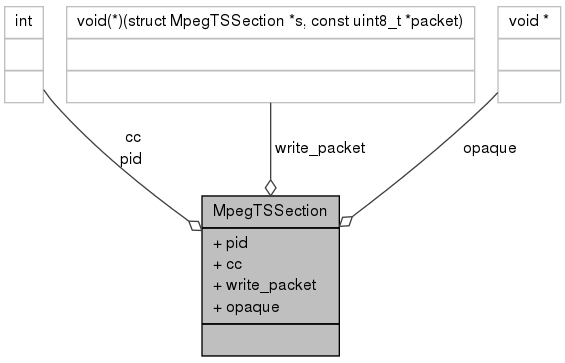
\includegraphics[width=0.8\linewidth]{figuras/structMpegTSSection__coll__graph.png}
\\Source: Automatically generated with Doxygen from the source code.
\label{fig:structMpegTSSection__coll__graph}
\end{figure}

\texttt{MpegTSService} represents a service, and contains a \texttt{MpegTSSection} for its Program Map Table, a service ID, the PCR PID and a pair of control variables to manage the service's PCR transmission rate. The class diagram of this structure and its heritage relations is shown in \autoref{fig:structMpegTSService__coll__graph}.

\begin{figure}[!b]
\centering
\caption{Class diagram for MpegTSService structure.}
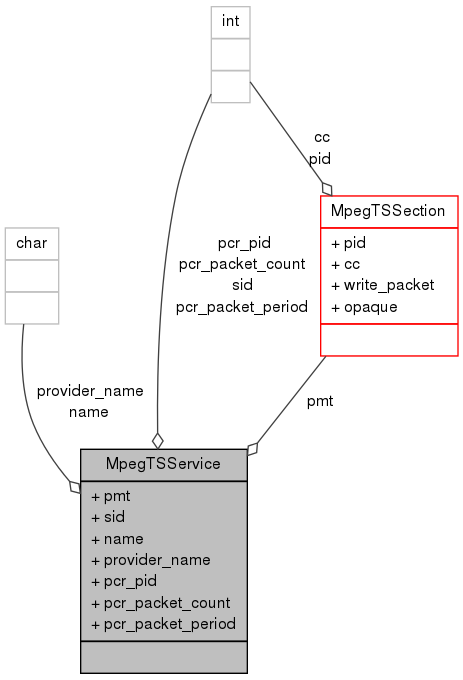
\includegraphics[width=0.8\linewidth]{figuras/structMpegTSService__coll__graph.png}
\\Source: Automatically generated with Doxygen from the source code.
\label{fig:structMpegTSService__coll__graph}
\end{figure}

\texttt{MpegTSWriteStream} represents one elementary stream that is sent through the TS. It has a pointer to the corresponding service, the stream PID, a continuity counter, the stream's current PTS and DTS values and the stream raw payload itself. The class diagram of this structure and its heritage relations is shown in \autoref{fig:structMpegTSWriteStream__coll__graph}.

\begin{figure}[!b]
\centering
\caption{Class diagram for MpegTSWriteStream structure.}
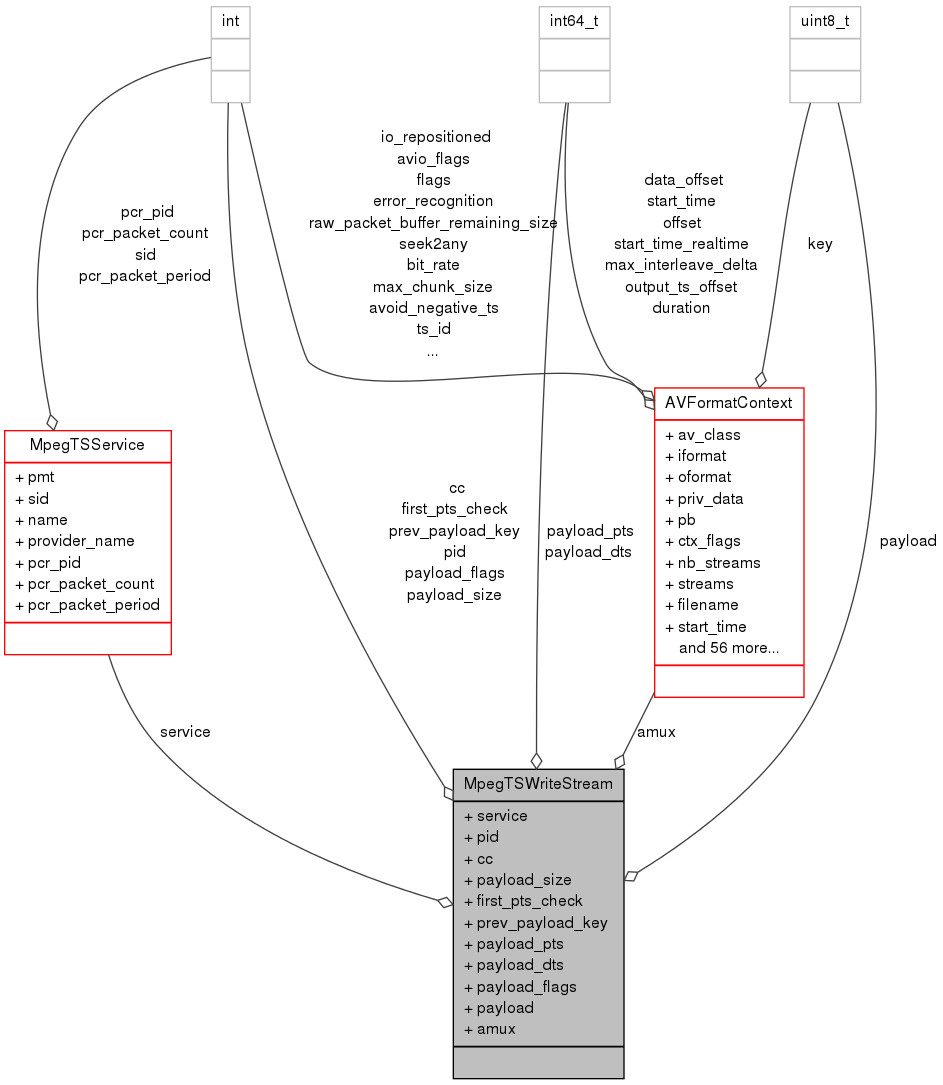
\includegraphics[width=0.9\linewidth]{figuras/structMpegTSWriteStream__coll__graph.png}
\\Source: Automatically generated with Doxygen from the source code.
\label{fig:structMpegTSWriteStream__coll__graph}
\end{figure}

The main multiplexer structure is \texttt{MpegTSWrite}, shown in \autoref{lst_MpegTSWrite}, that represents the Transport Stream itself. The structure contains the PSI tables PAT, NIT and SDT as three \texttt{MpegTSSection} structures, a dynamic array of \texttt{MpegTSServices} and many control variables, such as the counter \texttt{nb\hspace{0.1mm}\_\hspace{0.1mm}services} for the number of services contained in the TS, the desired constant multiplexing rate \texttt{mux\hspace{0.1mm}\_\hspace{0.1mm}rate} and a pair of variables to control the repeated transmission of each PSI table.

Along with the control variables, the physical network information is included as well: the fields \texttt{transport\hspace{0.1mm}\_\hspace{0.1mm}stream\hspace{0.1mm}\_\hspace{0.1mm}id} and \texttt{original\hspace{0.1mm}\_\hspace{0.1mm}network\hspace{0.1mm}\_\hspace{0.1mm}id} are assigned values received from the command-line. The class diagram of this structure and its heritage relations is shown in \autoref{fig:structMpegTSWrite__coll__graph}.

\begin{figure}[H]
\centering
\caption{Class diagram for MpegTSWrite structure.}
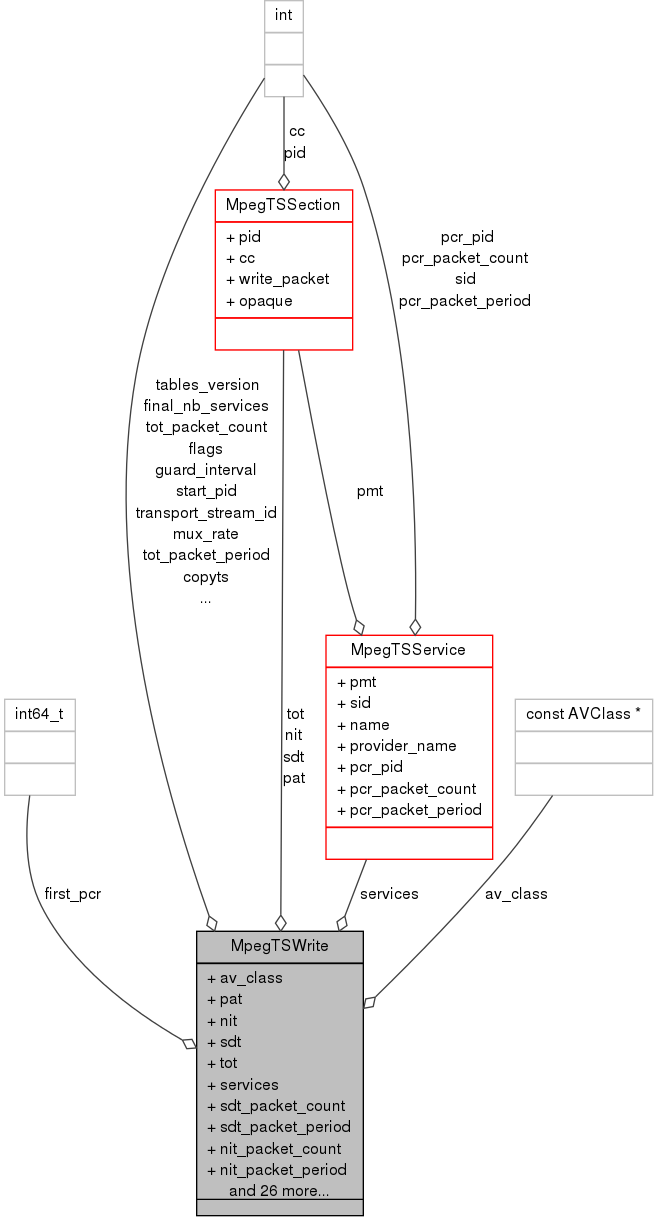
\includegraphics[width=0.7\linewidth]{figuras/structMpegTSWrite__coll__graph.png}
\\Source: Automatically generated with Doxygen from the source code.
\label{fig:structMpegTSWrite__coll__graph}
\end{figure}

Each command-line parameter passed to FFmpeg is parsed and must be validated before use. Each valid option is listed as one entry in a structure, an example is presented in \autoref{lst_input_option}. The first field is the option name, the second is a help text, the third is the position within a structure where it should be stored, then comes the variable type, the default value if it is not passed as argument, the minimum value, the maximum, and finally a internal definition of the option.

% By knowing the few information about FFMPEG muxer structures presented so far, one can already understand basically how the system works. A simple block diagram in Figure \ref{fig:diagrama_estruturas_ffmpeg} shows the relations between the presented structures, along with an example situation. Consider a digital television transport stream constituted by two services, with service IDs 1 and 2. The first service is formed by one video stream, with ID 101, and two audio streams, with IDs 111 and 112. The second service has one video stream, ID 201, and one audio stream, with ID 211. Each service has its own mapping table: for service 1 the table has a Table ID \(TID\) of 4001, and for service 2 the TID is 4002. Each program map table \(PMT\) links the service number to the stream numbers as defined by the standard. Finally, the program association table \(PAT\) links the available services 1 and 2 with their respective PMTs. To possibilitate the decoder to find these information within a transport stream, the PAT must have TID equal to 0, as can be noticed.

% \begin{figure}
% \centering
% \caption{Block diagram showing the relations between FFMPEG MPEG2 Muxer.}
% 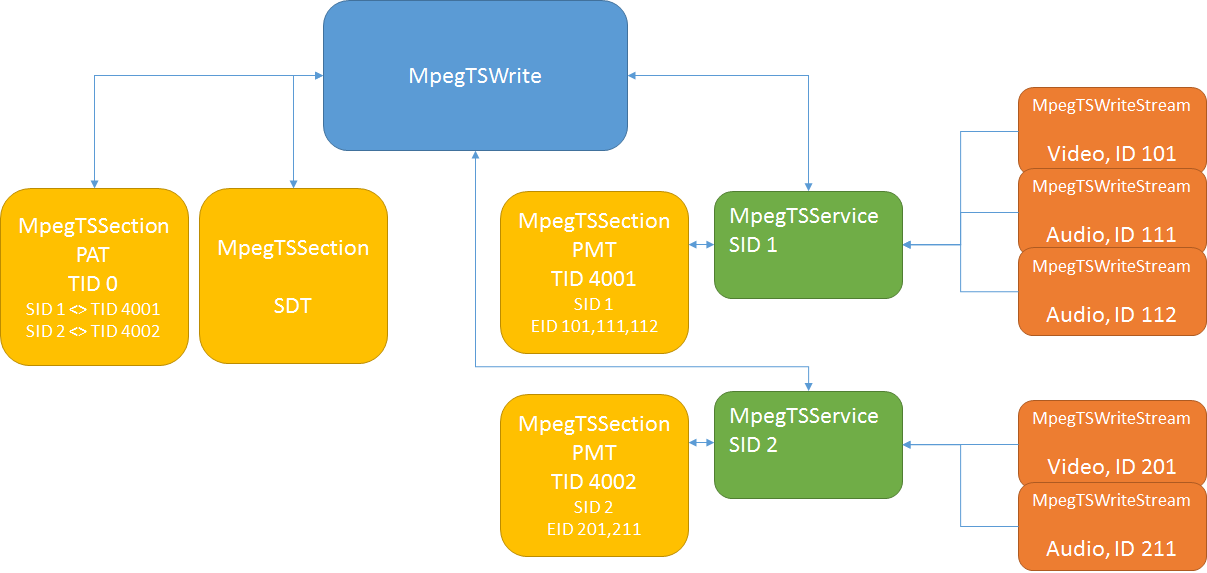
\includegraphics[width=1\linewidth]{figuras/diagrama_estruturas_ffmpeg.png}
% \\Source: the author.
% \label{fig:diagrama_estruturas_ffmpeg}
% \end{figure}

\subsection{Functions}

The main functions related to the multiplexing process are \texttt{av\hspace{0.1mm}\hspace{0.1mm}\_\hspace{0.1mm}\hspace{0.1mm}write\hspace{0.1mm}\hspace{0.1mm}\_\hspace{0.1mm}\hspace{0.1mm}header()} for writing the TS stream header, \texttt{av\hspace{0.1mm}\hspace{0.1mm}\_\hspace{0.1mm}\hspace{0.1mm}write\hspace{0.1mm}\hspace{0.1mm}\_\hspace{0.1mm}\hspace{0.1mm}packet()} for writing the packets and \texttt{av\hspace{0.1mm}\hspace{0.1mm}\_\hspace{0.1mm}\hspace{0.1mm}write\hspace{0.1mm}\hspace{0.1mm}\_\hspace{0.1mm}\hspace{0.1mm}trailer()} for writting the stream tail. The list below describes the sequence of the calls to the functions:

\begin{enumerate}
	\item{A call to \texttt{av\hspace{0.1mm}\_\hspace{0.1mm}write\hspace{0.1mm}\_\hspace{0.1mm}header()} initializes the control variables;}
	\item{as long as there is available data in the input streams, successive calls to \texttt{av\hspace{0.1mm}\_\hspace{0.1mm}write\hspace{0.1mm}\_\hspace{0.1mm}packet()} occur, each one writes one 188-byte TS packet in the output \textit{.ts} file. In its turn, \texttt{av\hspace{0.1mm}\_\hspace{0.1mm}write\hspace{0.1mm}\_\hspace{0.1mm}packet()} calls \texttt{mpegts\hspace{0.1mm}\_\hspace{0.1mm}write\hspace{0.1mm}\_\hspace{0.1mm}pes()} to handle the writing process of the current TS packet:}
	\begin{enumerate}
		\item {\label{itm:ret_si_info} \texttt{mpegts\hspace{0.1mm}\_\hspace{0.1mm}write\hspace{0.1mm}\_\hspace{0.1mm}pes()} calls  \texttt{retransmit\hspace{0.1mm}\_\hspace{0.1mm}si\hspace{0.1mm}\_\hspace{0.1mm}info()}, that outputs one PSI table section in the packet, if it's time;}
		\item {\label{itm:dts_condition} \texttt{mpegts\hspace{0.1mm}\_\hspace{0.1mm}write\hspace{0.1mm}\_\hspace{0.1mm}pes()} loops among the streams and searches a stream with the current frame DTS within the time interval of the current PCR.}
	\end{enumerate}
	\item{when input streams are over, \texttt{av\hspace{0.1mm}\_\hspace{0.1mm}write\hspace{0.1mm}\_\hspace{0.1mm}end()} frees allocated memory and closes the files.}
\end{enumerate}

To decide if it's time, in \autoref{itm:ret_si_info}, \texttt{retransmit\hspace{0.1mm}\_\hspace{0.1mm}si\hspace{0.1mm}\_\hspace{0.1mm}info()} uses the control variables \texttt{*\hspace{0.1mm}\_\hspace{0.1mm}packet\hspace{0.1mm}\_\hspace{0.1mm}count} and \texttt{*\hspace{0.1mm}\_\hspace{0.1mm}packet\hspace{0.1mm}\_\hspace{0.1mm}period} of each table to control the transmission rates by incrementing the corresponding \texttt{packet\hspace{0.1mm}\_\hspace{0.1mm}count} each time the function is called and outputting the table only when the counter reaches \texttt{packet\hspace{0.1mm}\_\hspace{0.1mm}period};

In \autoref{itm:dts_condition}, if \texttt{mpegts\hspace{0.1mm}\_\hspace{0.1mm}write\hspace{0.1mm}\_\hspace{0.1mm}pes()} finds a suitable PES packet, it fills a TS packet with data from this stream. If not, \texttt{mpegts\hspace{0.1mm}\_\hspace{0.1mm}write\hspace{0.1mm}\_\hspace{0.1mm}pes()} \texttt{mpegts\hspace{0.1mm}\_\hspace{0.1mm}insert\hspace{0.1mm}\_\hspace{0.1mm}pcr\hspace{0.1mm}\_\hspace{0.1mm}only()} is called to output only the necessary for a single PCR, without PES payload nor PSI tables, or \texttt{mpegts\hspace{0.1mm}\_\hspace{0.1mm}insert\hspace{0.1mm}\_\hspace{0.1mm}null\hspace{0.1mm}\_\hspace{0.1mm}packet()} is called to output an empty TS packet, full of stuffing bytes.

FFmpeg has dedicated functions to write TS packets with PSI tables. \texttt{mpegts\hspace{0.1mm}\_\hspace{0.1mm}write\hspace{0.1mm}\_\hspace{0.1mm}section()} is responsible for writing the TS packet header fields described in \autoref{ts_header}. \texttt{mpegts\hspace{0.1mm}\_\hspace{0.1mm}write\hspace{0.1mm}\_\hspace{0.1mm}section1()} is responsible for writing the common fields for all PSI tables, described in \autoref{iso_psi}.

%and \autoref{abnt_psi}

% ----------------------------------------------------------
% PARTE
% ----------------------------------------------------------
%\part{Resultados}
% ----------------------------------------------------------

% ---
% development
% ---
% ---

%Find: \hspace{0.1mm}\_\hspace{0.1mm}
% Replace with: \hspace{0.1mm}\hspace{0.1mm}\_\hspace{0.1mm}\hspace{0.1mm}

\section{New input options}
In order to provide flexibility to the user to configure the Transport Stream parameters according to his needs, several options were added to the command-line interface.

Most of them materialize the physical characteristics of the network and their names are very related to the definitions in the standards: \texttt{mpegts\hspace{0.1mm}\hspace{0.1mm}\_\hspace{0.1mm}\hspace{0.1mm}transport\hspace{0.1mm}\hspace{0.1mm}\_\hspace{0.1mm}\hspace{0.1mm}stream\hspace{0.1mm}\hspace{0.1mm}\_\hspace{0.1mm}\hspace{0.1mm}id}, \texttt{mpegts\hspace{0.1mm}\hspace{0.1mm}\_\hspace{0.1mm}\hspace{0.1mm}original\hspace{0.1mm}\hspace{0.1mm}\_\hspace{0.1mm}\hspace{0.1mm}network\hspace{0.1mm}\hspace{0.1mm}\_\hspace{0.1mm}\hspace{0.1mm}id}, \texttt{mpegts\hspace{0.1mm}\hspace{0.1mm}\_\hspace{0.1mm}\hspace{0.1mm}area\hspace{0.1mm}\hspace{0.1mm}\_\hspace{0.1mm}\hspace{0.1mm}code}, \texttt{mpegts\hspace{0.1mm}\hspace{0.1mm}\_\hspace{0.1mm}\hspace{0.1mm}guard\hspace{0.1mm}\hspace{0.1mm}\_\hspace{0.1mm}\hspace{0.1mm}interval}, \texttt{mpegts\hspace{0.1mm}\hspace{0.1mm}\_\hspace{0.1mm}\hspace{0.1mm}transmission\hspace{0.1mm}\hspace{0.1mm}\_\hspace{0.1mm}\hspace{0.1mm}mode}, \texttt{mpegts\hspace{0.1mm}\hspace{0.1mm}\_\hspace{0.1mm}\hspace{0.1mm}physical\hspace{0.1mm}\hspace{0.1mm}\_\hspace{0.1mm}\hspace{0.1mm}channel}, \texttt{mpegts\hspace{0.1mm}\hspace{0.1mm}\_\hspace{0.1mm}\hspace{0.1mm}virtual\hspace{0.1mm}\hspace{0.1mm}\_\hspace{0.1mm}\hspace{0.1mm}channel}.

Others are used as control variables and are self-explanatory: \texttt{mpegts\hspace{0.1mm}\hspace{0.1mm}\_\hspace{0.1mm}\hspace{0.1mm}final\hspace{0.1mm}\hspace{0.1mm}\_\hspace{0.1mm}\hspace{0.1mm}nb\hspace{0.1mm}\hspace{0.1mm}\_\hspace{0.1mm}\hspace{0.1mm}services} and \texttt{mpegts\hspace{0.1mm}\hspace{0.1mm}\_\hspace{0.1mm}\hspace{0.1mm}transmission\hspace{0.1mm}\hspace{0.1mm}\_\hspace{0.1mm}\hspace{0.1mm}profile}. Their use is explained in the following sections.

% ---
\section{Multiple services}
% ---

\subsection{Introduction}

The first proposed modification to the original FFMPEG code is to add multiple service support. The first task was to find a way to give to the multiplexer new information about how many services should be generated. This was done by creating a new command-line parameter: the option \texttt{mpegts\hspace{0.1mm}\_\hspace{0.1mm}transmission\hspace{0.1mm}\_\hspace{0.1mm}profile}.

Two profiles were designed:
\begin{itemize}
\item profile number '1' was designed with two services: one Full-segment service with a high-definition video stream and an audio stream and one 1-Segment service with a low-definition video stream and another audio stream;
\item profile number '2' was designed with a variable number of services: up to four services, each with a standard-definition video stream and an audio stream; and one  1-Segment service with a low-definition video stream and another audio stream.
\end{itemize}

Further information about the Full-Segment and 1-Segment services are provided in \autoref{modulation}.

\subsection{Profile 1: one Full-seg service and one 1-Seg service}

First the service ID for the HDTV service is calculated, based on the definitions in \autoref{special_fields}: the network ID is the \texttt{ts->onid} variable; the service type is hard-coded as \texttt{'00'}, as well as the program number (\texttt{0x0}). Then, one \texttt{MpegTSService} is added to the services array in \texttt{MpegTSWrite} with the existent \texttt{mpegts\hspace{0.1mm}\_\hspace{0.1mm}add\hspace{0.1mm}\_\hspace{0.1mm}service()} function. The parameters to this function are the recent calculated HD service ID, the provider name and the hard-coded service name. The process is repeated for the 1-Segment service, except that the service type is coded as \texttt{'11'} and the program number as \texttt{0x1}. Finally, the variable \texttt{ts->final\hspace{0.1mm}\_\hspace{0.1mm}nb\hspace{0.1mm}\_\hspace{0.1mm}services} is set as \texttt{'2'}.

\subsection{Profile 2: standard definition services and one 1-Seg service}

Profile two is not yet implemented, but the guidelines are the same as for profile 1. Instead of setting the variable \texttt{ts->final\hspace{0.1mm}\_\hspace{0.1mm}nb\hspace{0.1mm}\_\hspace{0.1mm}services} as 2, the value is left free for the user to choose and instead of creating only two services, a loop iterates the service creation until a counter reaches the total number of services.

\subsection{Stream Mapping}
\label{stream_mapping}

When calling FFmpeg, the user defines the order that input streams shall be placed in the \texttt{AVFormatContext} structure with the \texttt{-map} option. This same sequence is used in the streams loops throughout the code, and defines also the order of assignment of streams PIDs. The first input stream receives the value in \texttt{mpegts\hspace{0.1mm}\_\hspace{0.1mm}pmt\hspace{0.1mm}\_\hspace{0.1mm}start\hspace{0.1mm}\_\hspace{0.1mm}pid} and the value is incremented by one for each new stream. The default value for \texttt{mpegts\hspace{0.1mm}\_\hspace{0.1mm}pmt\hspace{0.1mm}\_\hspace{0.1mm}start\hspace{0.1mm}\_\hspace{0.1mm}pid} is \texttt{0x100}.

As already explained, streams hold the information of which service contains them with a pointer to one \texttt{MpegTSService} instance within the \texttt{MpegTSWriteStream} structure. Before the modifications of this project, since there was only one service, all the streams belonged to it. Now, the multiplexer iterates through all the streams and does a modulus operation with the stream index and the value of \texttt{mpegts\hspace{0.1mm}\_\hspace{0.1mm}final\hspace{0.1mm}\_\hspace{0.1mm}nb\hspace{0.1mm}\_\hspace{0.1mm}services} to assign alternately one stream to each service, as shown in \autoref{lst_stream_assignment}. \texttt{ts\hspace{0.1mm}\_\hspace{0.1mm}st} is the stream structure, \texttt{i} is the iteration variable.

\begin{minipage}{\linewidth}
\begin{lstlisting}[caption={Assigning streams to services.}, label={lst_stream_assignment}]
ts_st->service = ts->services[i % ts->final_nb_services];
\end{lstlisting}
\end{minipage}

%Considering the example shown in Figure \ref{fig:diagrama_estruturas_ffmpeg}, 
The mapping should be done by placing first the two video streams, then the first audio stream corresponding to the first service, then the audio stream corresponding to the second service and finally the second audio stream corresponding to the first service.

\section{PSI tables}

%\subsection{Introduction}
Each time \texttt{retransmit\hspace{0.1mm}\_\hspace{0.1mm}si\hspace{0.1mm}\_\hspace{0.1mm}info()} is called, it updates the counters for each table and tests if they have reached the period value. If true, \texttt{retransmit\hspace{0.1mm}\_\hspace{0.1mm}si\hspace{0.1mm}\_\hspace{0.1mm}info()} calls the \texttt{mpegts\hspace{0.1mm}\_\hspace{0.1mm}write\hspace{0.1mm}\_\hspace{0.1mm}<table>()} function, where \texttt{<table>} is one of the following: \texttt{sdt, nit, tot, pat, pmt}. To add SDT, NIT and TOT support, three sets of conditional calls were added, similar to the one shown in \autoref{lst_write_table_call}.

\begin{minipage}{\linewidth}
\begin{lstlisting}[caption={Conditional call to \texttt{mpegts\hspace{0.1mm}\_\hspace{0.1mm}write\hspace{0.1mm}\_\hspace{0.1mm}nit()}.}, label={lst_write_table_call}]
if (++ts->nit_packet_count == ts->nit_packet_period) {
    ts->nit_packet_count = 0;
    mpegts_write_nit(s);
}
\end{lstlisting}
\end{minipage}

A set of macros were added to hold the default values of network characteristics, shown in \autoref{lst_macros}. In C language, when an array variable is declared, a memory area with the size of the array is allocated and the variable itself is a pointer to the first element of the array \citeonline[5.1]{ritchie}. ISO defines 1024 bytes as the maximum authorized length of a table \citeonline[2.4.4]{ISO}. Excluding 8 bytes of the table header and 4 bytes of the CRC, results in 1012 bytes.

To create the bitstream of the table with pointer manipulation, first an array of type \texttt{uint8\hspace{0.1mm}\_\hspace{0.1mm}t}\footnote{\texttt{uint8\hspace{0.1mm}\_\hspace{0.1mm}t} is an unsigned integer type with size of 1 byte.} with 1012 bytes is declared with name \texttt{data}. Then a pointer \texttt{q} of the same type is declared and the first address of the array is assigned to it.

Since all the bytes in the array are stored in a contiguous memory area, it is easy to create the table bitstream by assigning the byte value of the address pointed by \texttt{q} and incrementing the pointer after each assignment, so that the next assignment is done in the next byte of the array. Since section length is dependant on how many bytes are used and length fields are at the beginning of the headers, length fields are skipped in a first pass to be filled later, and an auxiliary pointer(\texttt{len\hspace{0.1mm}\_\hspace{0.1mm}ptr}) holds the position of the length fields for the second pass. 

\subsection{Length Calculation}
\label{length_calc}

Section lengths are calculated in a simple way. Most of the time their value only counts the variable size part of the sections, from right after the length field and up to the end of the last byte of the section. By calculating the difference of the two pointers \texttt{q} and \texttt{len\hspace{0.1mm}\_\hspace{0.1mm}ptr}, one gets the number of bytes written including length bytes. If one subtracts the size of the length field from this difference, he easily obtains the length of the variable portion of the section.

\autoref{lst_pointer_assignment} shows an excerpt of the code: the pointer assignment algorithm. \autoref{fig:pointer_assignment} shows an example of how the  algorithm works. Six of the bytes allocated to variable \texttt{data} are shown on top, empty.
\begin{enumerate}
\item The first \texttt{data} address is assigned to \texttt{q} , as shown by the continuous arrow.
\item \label{itm:len_ptr1} The syntax shown assigns the value \texttt{0x10} to the address pointed by \texttt{q} and increments by one the pointed address. The continuous arrow shows the pointed address after \autoref{itm:len_ptr1} is completed.
\item \label{itm:len_ptr2} \texttt{len\hspace{0.1mm}\_\hspace{0.1mm}ptr} stores the current position of \texttt{q}, as indicated by the dashed arrow; the address pointed to by \texttt{q} is incremented by 2 units, as indicated by the continuous arrow, to leave space to the length fields.
\item the value \texttt{0x45} is stored in the address currently pointed by \texttt{q}, and \texttt{q} is incremented by 1 byte.
\item after all fields are filled with data and the length of the section is known, the length is written using the auxiliary pointer \texttt{len\hspace{0.1mm}\_\hspace{0.1mm}ptr}, that remains pointing to the same position defined in \autoref{itm:len_ptr2}.
\end{enumerate}

\begin{figure}[!h]
\centering
\caption{Pointer assignment example.}
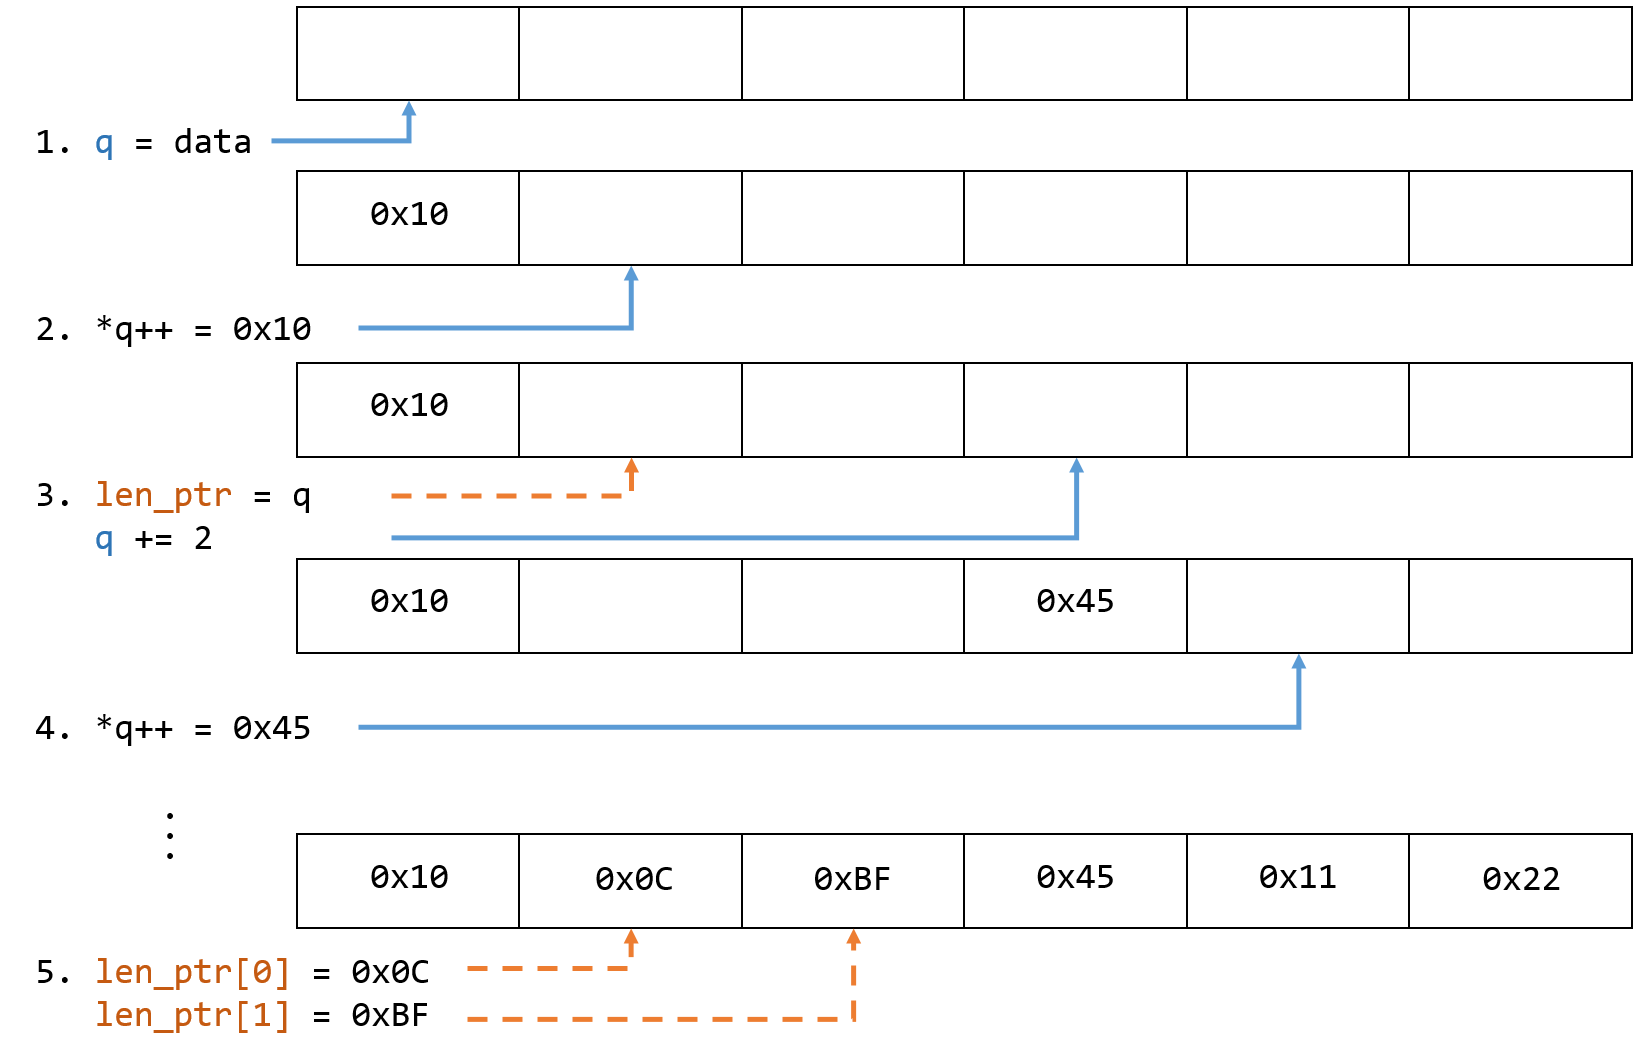
\includegraphics[width=0.8\linewidth]{figuras/pointer_assignment.png}
\\Source: The author.
\label{fig:pointer_assignment}
\end{figure}

\subsection{Descriptors}

In order to facilitate the creation of the descriptors, a prototype of C code was written. It is presented in \autoref{lst_proto_desc}. This was possible because the descriptors syntax follow a regular syntax, they always start with a tag byte, followed by a length field with one or two bytes, and followed by data bytes. The calculation of descriptors lengths use the same algorithm described in \autoref{length_calc}. All the descriptors in tables from PSI/SI which were described in theoretical sections were coded in the application.

\begin{minipage}{\linewidth}
\begin{lstlisting}[caption={Descriptors prototype.}, label={lst_proto_desc}]
	*q++ = 0x;
	_length_ptr = q;
	*q++;
	put16(&q, 0x);
	*q++ = 0x; 
_length_ptr[0] = q - _length_ptr - 1;
\end{lstlisting}
\end{minipage}

%% ---
%%  capitulo de Resultados
%% ---
\chapter{Tests and Results}
%% ---
%
%% ---
\section{Test environment}

The laboratory disposes of two systems for TV broadcasting: the first is an EiTV Playout Laboratory \cite{eitv}, that comprises a PSI/SI generator, a multiplexer, a modulator and a low power transmitter. It is a commercial solution, which meets the technical requirements of the SBTVD but the source code is not open to contribution. As inputs, one may supply one or more single-service TS streams as binary files containing video and audio ESs and fill data into forms to be added to the PSI and SI tables. It does not allow input TS files to contain multiple services, so to broadcast a multi-service stream one may only use the internal multiplexer.

As output, the multiplexer produces either a single service or a multi service stream, depending on how the input streams were configured, and the TS is sent in real-time to the modulator and the transmitter.This solution is not totally adapted to the project, since it does not allow multiple services in the same input TS. It is useful, on the other hand, to test the timing of audio and video streams.

The other available solution in the Dektec DTA-115 PCI modulator board, which is installed in a PC workstation. This device is much more adapted to the project goals, because it receives a multi-service Transport Stream as binary file and performs the modulation and transmission steps. It's output is a RF connector which is currently connected to a  UHF antenna. A complete description of the board is available in the manufacturer's website \cite{dektec}. The control of the board is done using StreamXpress software, provided by the board's manufacturer.

% \begin{figure}[!hb]
% \centering
% \caption{Input points for the available solutions.}
% 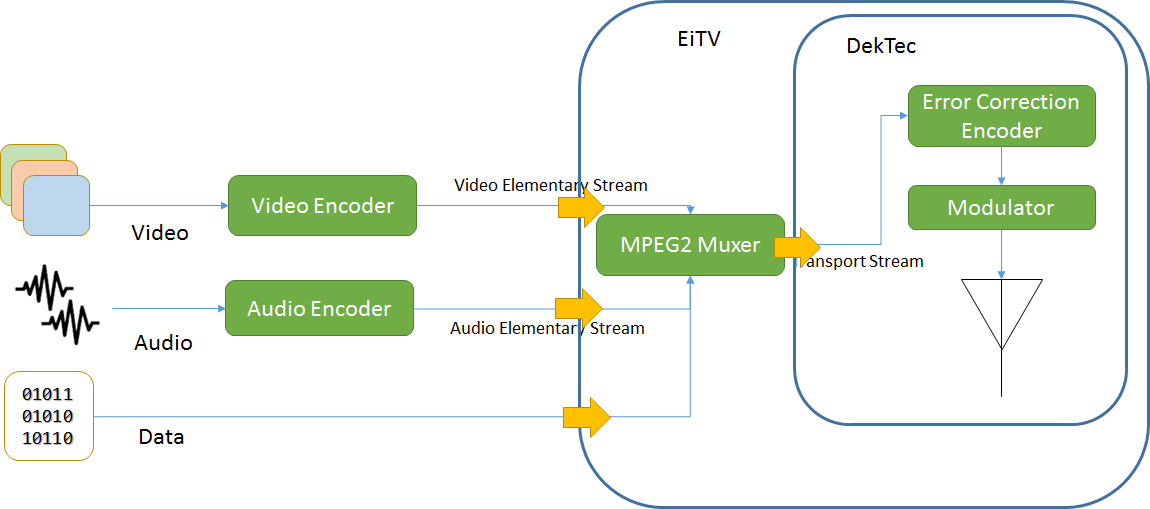
\includegraphics[width=0.9\linewidth]{figuras/scope_eitv_dektec.png}
% \\Source: The author.
% \label{fig:scope_eitv_dektec}
% \end{figure}

Two visualization devices are available for each service type: a Philips LCD TV and an EiTV Set Top Box for Full-Segment reception and for 1-Segment reception a Lenoxx GPS with DTV and a Samsung Cell Phone with DTV. Additionally, a Pixelview PenTV USB receiver with Full-segment and 1-Segment reception capabilities is used attached to a Linux Workstation. With the USB receiver, Transport Streams are captured and then analysed using two free softwares: \textit{MPEG-2 TS Packet Analyser} and \textit{SBTVD Transport Stream Parser v0.32}. FFprobe is also used as a tool to analyse TSs and display information about the streams contained in them.

\section{Timing tests}

These tests were done before any modifications on the source code. The objective of these first tests is to verify that FFmpeg, without any modifications, can provide a stream with video and audio in sync. 

Two different sources of video and audio were tested. The first source is a \textit{mp4} file that contains a video encoded in H.264 with resolution of 720x404 pixels, 23.98 frames per second, and audio encoded in HE-AAC with stereo channels at a sample rate of 48KHz. The second source is another \textit{mp4} file with H.264 video, frame size of 480x360 pixels at 29.97 fps, and stereo HE-AAC audio at 48KHz. The two videos were re-encoded with FFmpeg to output a 1920x1080 frame size at 29,97 frames per second, and the MPEG2 multiplexer was used to create a Transport Stream with one single service. The block diagram in \autoref{fig:test_scn_timing} shows the signal flow.

\begin{figure}[!hb]
\centering
\caption{Signal flow for timing tests.}
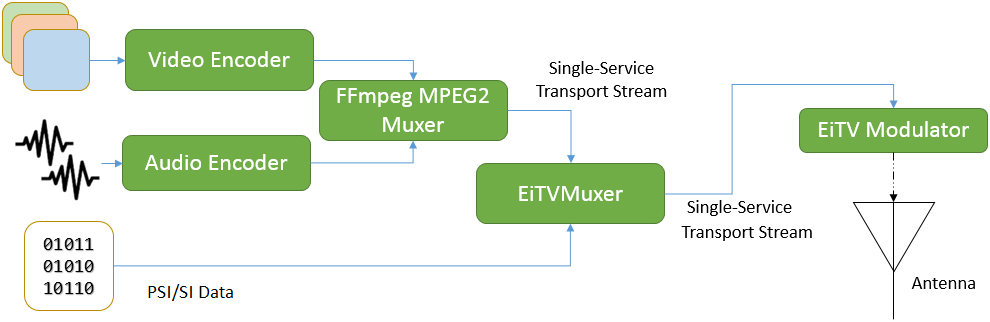
\includegraphics[width=0.9\linewidth]{figuras/test_scn_timing.png}
\\Source: The author.
\label{fig:test_scn_timing}
\end{figure}

The syntax to call ffmpeg and produce these outputs is shown in \autoref{lst_ffmpeg_single_service}. \texttt{-vcodec libx264 -r 29.97 -s hd1080 -profile:v high} set up the video codec. \texttt{-acodec aac -strict -2 -latm 1} set up the audio codec. \texttt{-t 60} tells the multiplexer to generate a TS with only 60 seconds.

\begin{minipage}{\linewidth}
\begin{lstlisting}[caption={Single Service TS creation with FFmpeg.}, label={lst_ffmpeg_single_service}]
./ffmpeg -i src.mp4 -vcodec libx264 -r 29.97 -s hd1080 -profile:v high -acodec aac -strict -2 -latm 1 -muxrate 3600000 -t 60 -mpegts_flags latm -loglevel verbose -y dst.ts
\end{lstlisting}
\end{minipage}

Attention should be given to the importance of the \texttt{muxrate} option. In the first repetitions of this test, FFmpeg was being called without this option and the output TS ended up with a variable bitrate (VBR), which is not compliant to the MPEG2 standard and leads to a catastrophic loss of sync. When setting up the transmission parameters in EiTV control panel, the TS bitrate must be entered, so the average bitrate of the stream was applied. Since a VBR TS was being broadcast as if it had constant bitrate (CBR), whenever the output bitrate was greater than input bitrate, frames were presented faster than supposed to or skipped. On the opposite case, there were gaps without any frame and the audio would mute or the video would freeze.

After realizing the need of setting muxrate, it was necessary to know what value should be set. If an underestimated bit-rate is chosen, the PCRs and PTSs will be calculated incorrectly and frames will not be delivered at the expected frame rate. When the transmitter eventually sends the bit-stream to the air in a slower bitrate than necessary, playback will present freeze moments because there will be instants of time without video or audio to be displayed, i.e., it is as if the stream was reproduced in slow motion. On the other hand, an overestimated TS bit-rate causes the multiplexer to add too much stuffing packets into the stream and use unnecessary band.

Analyses of the local broadcast channel shown that TSs carried about 11 \% of stuffing bytes, as can be shown in the graphics in \autoref{fig:graph_rbs_dump} and \autoref{fig:graph_band_dump}. The percentages indicated in the figures refer to the amount of data in each PIDs. The PID numbers and packet counts can be seen in \autoref{tab_dumps}. In the graphs, the designation of stuffing packets is \textit{null packet}. From this information, the muxrate option was set at 3.6 Mbps, which results in an overhead of about 11 \%, as can be seen in \autoref{fig:graph_generated_dump}.

\begin{figure}[!h]
\centering
\caption{Packets distribution among PIDs in local broadcaster A.}
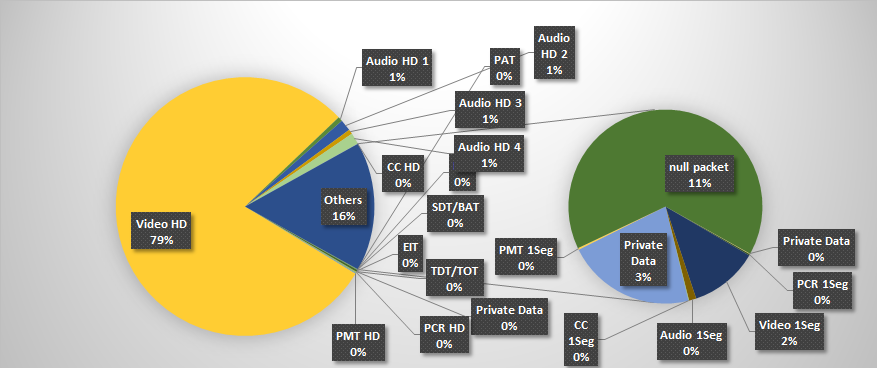
\includegraphics[width=0.9\linewidth]{figuras/graph_rbs_dump.png}
\\Source: The author.
\label{fig:graph_rbs_dump}
\end{figure}

\begin{figure}[!h]
\centering
\caption{Packets distribution among PIDs in local broadcaster B.}
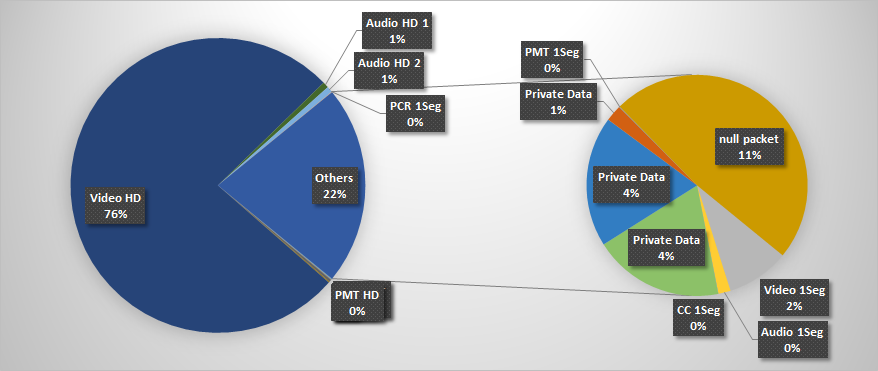
\includegraphics[width=0.9\linewidth]{figuras/graph_band_dump.png}
\\Source: The author.
\label{fig:graph_band_dump}
\end{figure}

\begin{table}[b]
\centering
    \caption {Data from stream aquisitions.}
    \begin{tabular}{|l|l|l|l|l|l|l|}
    \hline
     Bcaster A  & Bcaster A          & Bcaster A    & ~ & Bcaster B & Bcaster B         & Bcaster B   \\ \hline
    PID   & Type         & Count  & ~ & PID  & Type         & Count  \\ \hline
    0     & PAT          & 260    & ~ & 0    & PAT          & 100    \\ \hline
    16    & NIT          & 26     & ~ & 16   & NIT          & 10     \\ \hline
    17    & SDT/BAT      & 13     & ~ & 17   & SDT/BAT      & 5      \\ \hline
    18    & EIT          & 734    & ~ & 18   & EIT          & 10     \\ \hline
    20    & TDT/TOT      & 5      & ~ & 20   & TDT/TOT      & 2      \\ \hline
    39    & Private Data & 115    & ~ & 36   & ~            & 10     \\ \hline
    256   & PCR HD       & 452    & ~ & 39   & ~            & 10     \\ \hline
    257   & PMT HD       & 261    & ~ & 233  & CC HD        & 27     \\ \hline
    273   & Video HD     & 237551 & ~ & 256  & PCR HD       & 264    \\ \hline
    274   & Audio HD 1   & 1729   & ~ & 257  & PMT HD       & 100    \\ \hline
    275   & Audio HD 2   & 4288   & ~ & 273  & Video HD     & 76284  \\ \hline
    276   & Audio HD 3   & 1745   & ~ & 274  & Audio HD 1   & 654    \\ \hline
    277   & Audio HD 4   & 4280   & ~ & 275  & Audio HD 2   & 660    \\ \hline
    278   & CC HD        & 53     & ~ & 512  & PCR 1Seg     & 47     \\ \hline
    500   & Private Data & 51     & ~ & 529  & Video 1Seg   & 2006   \\ \hline
    512   & PCR 1Seg     & 114    & ~ & 530  & Audio 1Seg   & 394    \\ \hline
    529   & Video 1Seg   & 5551   & ~ & 549  & CC 1Seg      & 4      \\ \hline
    530   & Audio 1Seg   & 585    & ~ & 1000 & Private Data & 4169   \\ \hline
    534   & CC 1Seg      & 53     & ~ & 1001 & Private Data & 4168   \\ \hline
    900   & Private Data & 10415  & ~ & 4101 & Private Data & 521    \\ \hline
    8136  & PMT 1Seg     & 132    & ~ & 8136 & PMT 1Seg     & 26     \\ \hline
    8191  & null packet  & 31587  & ~ & 8191 & null packet  & 10529  \\ \hline
    Total & ~            & 300000 & ~ & ~    & ~            & 100000 \\ \hline
    \end{tabular}
	\label{tab_dumps}
\end{table}

\begin{figure}[!h]
\centering
\caption{Packets distribution among PIDs in generated TS.}
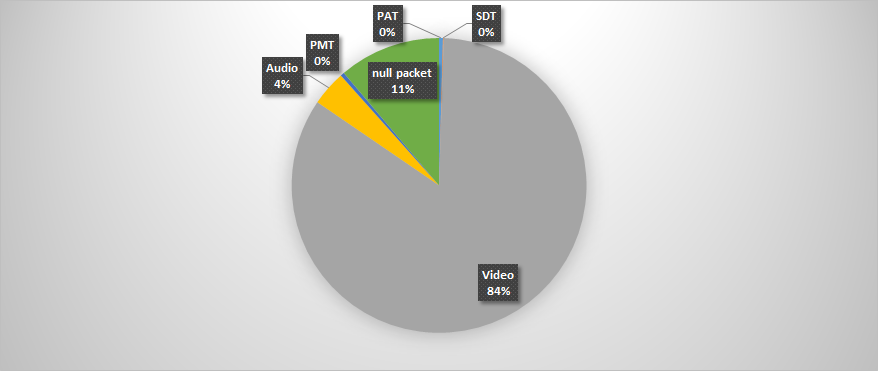
\includegraphics[width=0.9\linewidth]{figuras/graph_generated_dump.png}
\\Source: The author.
\label{fig:graph_generated_dump}
\end{figure}

\begin{minipage}{\linewidth}
\begin{lstlisting}[caption={Output of FFmpeg when input is as \autoref{lst_ffmpeg_single_service}.}, label={lst_ffprobe_clean}]
Input #0, mpegts, from 'dst.ts':
  Duration: 00:00:59.98, start: 1.445400, bitrate: 3662 kb/s
  Program 1 
    Metadata:
      service_name    : Service01
      service_provider: FFmpeg
    Stream #0:0[0x100]: Video: h264 (High) ([27][0][0][0] / 0x001B), yuv420p, 1920x1080, 29.97 fps, 29.97 tbr, 90k tbn, 59.94 tbc
    Stream #0:1[0x101](und): Audio: aac_latm ([17][0][0][0] / 0x0011), 48000 Hz, stereo, fltp
\end{lstlisting}
\end{minipage}

FFprobe displays what is in \autoref{lst_ffprobe_clean} when analysing the output of \autoref{lst_ffmpeg_single_service}. The TS lasts 59.98 seconds and has a bitrate of 3662 kbps. It contains only one program, with program\hspace{0.1mm}\_\hspace{0.1mm}number 1, that has two streams: one video stream (PID \texttt{0x100}) and one audio stream (PID \texttt{0x101}) that comply to the requirements of the SBTVD standard.

The streams were received in the visualization devices and the sync between video and audio was verified by watching and hearing the outputs in scenes where people were filmed while talking. Three different people stated that video and audio were in sync.

The results were satisfactory, and although there was no employment of functionalities developed by the author, this test was necessary to ensure that the multiplexer could packetize correctly the chunks of data, as well as label the frames with timestamps in sync.

%This TS is not compliant with the SBTVD standard. It does not contain the tables added in the development of the project and can not be used directly in DekTec board. They were remultiplexed in EiTV Playout, where the PSI tables were added, and then broadcasted. 
% a value of 18Mbps, which is much higher than the original re-encoded stream (2728 kbps) was passed as argument and the issue of muting audio and freezing video was solved, but it still caused video and audio to be completely out of sync. In dialog scenes, the characters' mouths would open several seconds after their voice was heard. Several analyses of the generated TSs with \textit{MPEG-2 TS Packet Analyser}, varying the muxrate values from 18Mbps down to 4Mbps. When 4Mbps was broadcast, audio and video became synced. Also, chunks of stuffing packets are placed by FFmpeg between chunks of different PIDs, so that audio and video streams are separated by long periods of stuffing packets.
% This was attributed to the fact that stuffing packets were 
% amount of stuffing packets added in the stream reduced after each reduction of muxrate, which is obvious. 
% To present streams in sync, the decoder must delay the presentation of one stream while waiting the arrival of the other stream. When too much stuffing packets are transmitted, the decoder can not wait so much time due to the size of their buffers, 

%\section{Analysing TS packets with Stream Analyser}

\section{Multiple Services Tests}

These tests were carried out after applying the implementations described in \autoref{implementation}. Their purpose is to validate the developed system. Two different sets of tests were made, one with a TS captured from a local broadcast channel with the USB receiver and the other with a TS created with the developed multiplexer.

\subsection{Retransmitting a captured TS}
\label{retransmitting}

This first set of tests were carried out to understand how the Dektec PCI board works and to validate its functioning. It was done by transmitting a TS that certainly is compliant to the standard, because it was captured from a local broadcaster. The simple block diagram in \autoref{fig:test_scn_retrans} shows the signal flow in this test.

\begin{figure}[!h]
\centering
\caption{Signal flow for retransmission tests.}
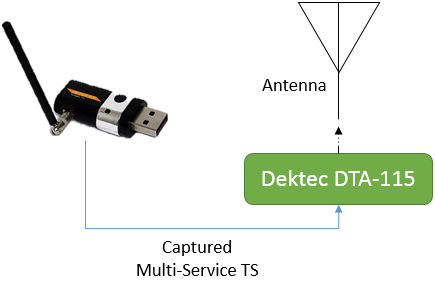
\includegraphics[width=0.5\linewidth]{figuras/test_scn_retrans.png}
\\Source: The author.
\label{fig:test_scn_retrans}
\end{figure}

The modulator board was configured with the following configuration, which is known to work as informed by previous researchers of the laboratory:

\begin{itemize}
\item television broadcast type, mode 3, guard interval 1/16;
\item partial reception enabled for 1-Segment transmission on layer A;
\item layer A configured with QPSK modulation, code rate 2/3, time interleave 2 and occupying one segment\footnote{\label{footnote_modulation}Refer to \autoref{modulation}.};
\item layer B configured with 64QAM modulation, code rate 3/4, time interleave of 2 and occupying twelve segments\footnotemark[\value{footnote}];
\end{itemize}

With the captured TS file loaded in StreamXpress and these configurations set, in the program interface it is possible to select which PIDs should really be transmitted and in which layer in real-time. Several different combinations of transmitted PIDs and the status of reception in the TV and cell phone are organized in the following tables. They are separated by the reception device and within each device separated by its tuning configuration.

\begin{table}
    \caption {TV receiver in manual tuning method.}
    \begin{center}
\begin{tabular}{|l|l|l|l|}
    \hline
    Sent PIDs                   & Signal Level & Screen / Speakers Status & Service Name \\ \hline
    NIT                         & 0            & Blue Screen              & NONE         \\ \hline
    NIT, PAT                    & Good         & Blue Screen              & NONE         \\ \hline
    NIT, PAT, PMT               & Good         & Blue Screen              & NONE         \\ \hline
    NIT, PAT, PMT, A/V ESs      & Good         & Video and Audio in Sync  & NONE         \\ \hline
    NIT, PAT, PMT, A/V ESs, SDT & Good         & Video and Audio in Sync  & HDTV SVC \\ \hline
    \end{tabular}
	\label{tab_manual_tuning}
\end{center}

\end{table}

\begin{table}
    \caption {TV receiver in normal operation mode.}
    \begin{center}
\begin{tabular}{|l|l|l|l|}
    \hline
    Sent PIDs               & Opens A/V & "No Signal" & "No available \\
                   & Streams & Flag & programme" flag \\ \hline
    NIT                     & NO                & YES              & NO                            \\ \hline
    NIT, PAT                & NO                & NO               & YES                           \\ \hline
    NIT, PAT, PMT           & NO                & NO               & YES                           \\ \hline
    NIT, PAT, PMT, Video ES & YES, video only   & NO               & NO                            \\ \hline
    NIT, PAT, A/V ESs  & NO         & NO               & YES                            \\ \hline
	NIT, PAT, PMT, A/V ESs  & YES, both         & NO               & NO                            \\ \hline
    \end{tabular}
	\label{tab_normal_operation}
\end{center}
\end{table}

\begin{table}
    \caption {TV receiver in blind search mode.}
    \begin{center}
\begin{tabular}{|l|l|}
    \hline
    Sent PIDs & Finds channel \\ \hline
    NIT       & YES           \\ \hline
    PAT, PMT  & NO            \\ \hline
    PAT       & NO            \\ \hline
    NIT, PAT  & YES           \\ \hline
    \end{tabular}
	\label{tab_blind_search}
\end{center}
\end{table}

Several important information can be observed from this tables:
\begin{itemize}
\item all times PAT and NIT were transmitted in layer A, so it can be noticed from \autoref{tab_manual_tuning} that the TV is capable of decoding PIDs sent in the 1-Segment layer;
\item during blind scan, the TV can not find the broadcast channel without the NIT as proved by \autoref{tab_blind_search};
\item in \autoref{tab_normal_operation}, without the PMT, even if the A/V ESs are sent, the TV can not open the streams;
\item the SDT doesn't make difference to the tuning or finding PIDs, but without it the service has no name.
\end{itemize}

%\autoref{tab_blind_search} 	\autoref{tab_normal_operation} 	\autoref{tab_manual_tuning}

With the cell phone, the results are slightly different. There is no manual tuning method, so only blind searches and normal operation tests were done. The results are:

\begin{itemize}
\item from \autoref{tab_cell} it can be seen that PAT presence makes no difference for the phone to open the streams. This is due to the recommendation on NBR 15608, for 1-Segment PMTs to have a default PID range;
\item without NIT, the phone can not find the broadcast channel in blind search. If NIT is removed after blind search, the phone keeps receiving as long as PMT is still being sent.
\end{itemize}

\begin{table}
    \caption {Cell phone in blind search and normal operation.}
    \begin{center}
\begin{tabular}{|l|l|l|}
    \hline
    Sent PIDs              & Finds channel in blind search & Status in normal operation \\ \hline
    NIT                    & YES                           & "Signal too weak, retry?"  \\ \hline
    PAT, PMT, SDT, A/V ESs & NO                            & Opens A/V                  \\ \hline
    NIT, PMT, SDT, A/V ESs & YES                           & Opens A/V                  \\ \hline
    NIT, PMT, A/V ESs      & YES                           & Opens A/V                  \\ \hline
    \end{tabular}
	\label{tab_cell}
\end{center}
\end{table}

This whole set of tests provides now information about what to expect when the stream generated by the developed multiplexer is broadcasted.

\subsection{Transmitting a remultiplexed TS with two services}
\label{test_remultiplexing}

The main objective of this last set of tests is to confirm that the developed multiplexer creates a TS compliant to the standard and that it is received and decoded correctly. The two inputs are edited Transport Streams which were captured and remultiplexed, one contains the Full Segment service and the other, the 1-Segment service. The signal flow is shown in \autoref{fig:test_scn_muxing}

\begin{figure}[!h]
\centering
\caption{Signal flow for remultiplexed TS tests.}
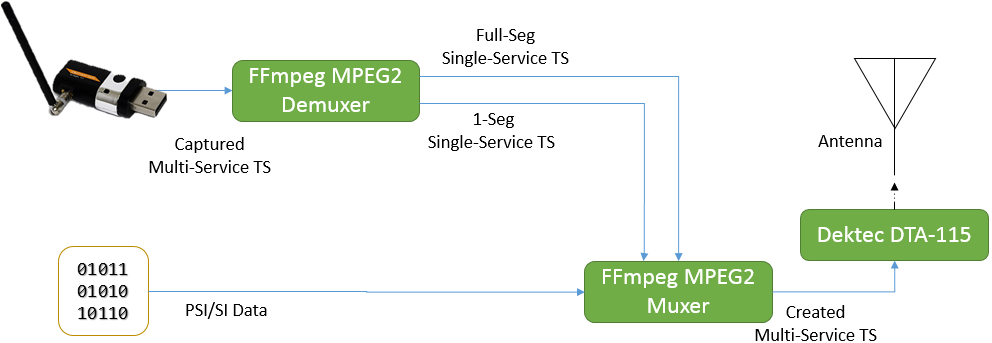
\includegraphics[width=0.8\linewidth]{figuras/test_scn_muxing.png}
\\Source: The author.
\label{fig:test_scn_muxing}
\end{figure}

The TS was generated using the following configurations, which are compliant to the standard: the physical network characteristics are original network ID 0730, area code 2970, guard interval 1/16, transmission mode 3, physical channel 20 and virtual channel 1. The transmission profile is set as 1. \autoref{lst_ffmpeg_multi_service} shows the command-line call and \autoref{lst_ffprobe_multi_service} shows the FFprobe analysis results.

\begin{minipage}{\linewidth}
\begin{lstlisting}[caption={FFmpeg command-line call to generate a multi-service TS}, label={lst_ffmpeg_multi_service}]
./ffmpeg -i /var/src/tve_HD_0406.ts -i /var/src/tve_LD_0406.ts -map 0:0 -map 1:0 -map 0:1 -map 1:1 -vcodec copy -acodec copy -mpegts_original_network_id 0730 -mpegts_area_code 2970 -mpegts_guard_interval 2 -mpegts_transmission_mode 3 -mpegts_physical_channel 20 -mpegts_virtual_channel 1 -mpegts_transmission_profile 1 -muxrate 12000000 -mpegts_flags latm -loglevel verbose -t 30 -y /home/nethome/endres/TVE_HD_LD.ts
\end{lstlisting}
\end{minipage}

\begin{minipage}{\linewidth}
\begin{lstlisting}[caption={FFprobe analysing the multi-service TS.}, label={lst_ffprobe_multi_service}]
Input #0, mpegts, from '/home/nethome/endres/TVE_HD_LD_long_1406.ts':
  Duration: 00:01:01.36, start: 1.400000, bitrate: 11972 kb/s
  Program 23360 
    Metadata:
      service_name    : SVC HD Full Seg
      service_provider: FFmpeg
    Stream #0:0[0x100]: Video: h264 (High) ([27][0][0][0] / 0x001B), yuv420p(tv, bt709), 1920x1080 [SAR 1:1 DAR 16:9], 29.97 fps, 29.97 tbr, 90k tbn, 59.94 tbc
    Stream #0:1[0x102](por): Audio: aac_latm ([17][0][0][0] / 0x0011), 48000 Hz, stereo, fltp
  Program 23385 
    Metadata:
      service_name    : SVC LD 1-Seg
      service_provider: FFmpeg
    Stream #0:2[0x101]: Video: h264 (Constrained Baseline) ([27][0][0][0] / 0x001B), yuv420p, 320x240 [SAR 1:1 DAR 4:3], 14.99 fps, 29.97 tbr, 90k tbn, 29.97 tbc
    Stream #0:3[0x103]: Audio: aac_latm ([17][0][0][0] / 0x0011), 48000 Hz, stereo, fltp
\end{lstlisting}
\end{minipage}

\begin{figure}[!h]
\centering
\caption{TS Parser output for four different Transport Streams.}
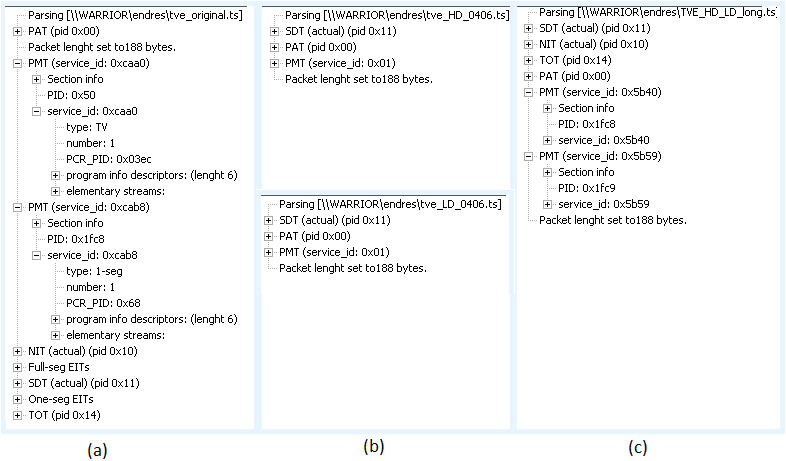
\includegraphics[width=0.9\linewidth]{figuras/ts_parser_tve_orig_remux.png}
\\Source: The author.
\label{fig:ts_parser_tve_orig_remux}
\end{figure}

\autoref{fig:ts_parser_tve_orig_remux} shows the output of MPEG2 Parser for the original captured TS in (a), the two streams derived from it in (b) and the remultiplexed TS by this project in (c). In (a), one may notice the presence of all PSI/SI tables. In (b), only one PMT remains on each edited TS and since they were generated with the original FFmpeg, SI tables are not present(NIT, TOT), except the SDT\footnote{An SDT without all the required information is generated by FFmpeg automatically.}. In (c), the PSI/SI tables are recreated with the developed solution and the service numbers are no longer the same, since network characteristics are different from the original captured TS.

In \autoref{fig:ts_parser_tve_remux_pmt} the TS Parser is analysing the PMTs of the remultiplexed TS. In the left side is the PMT for Full-Segment service, where service ID \texttt{0x5B40} can be identified, the parental rating descriptor is indicating that the show if free for all ages in Brazil and the Elementary Streams described are one video of type H.264 at PID \texttt{0x100} (the primary video ES) and one AAC/LATM audio of PID \texttt{0x102}. The parser lacks the syntax of some descriptors and can not show the AAC descriptor, for example, but it can be seen that its tag is \texttt{0x7C} and content is \texttt{0x2E} as indicated by \autoref{pmt_descriptors}.

In the right side of \autoref{fig:ts_parser_tve_remux_pmt}, the same as above is valid, but the video stream is identified as 1-segment primary video and the service number is \texttt{0x5B59}.

It is interesting to show here that the stream mapping explained in \autoref{stream_mapping} actually worked. The first input stream was the HD video and it received the PID \texttt{0x100}. The second was the 1-Segment video, assigned PID \texttt{0x101}. The third was HD audio, that got PID \texttt{0x102}, and 1-Segment audio got PID \texttt{0x103}.

\begin{figure}[!h]
\centering
\caption{TS Parser analysing PMTs of remultiplexed TS.}
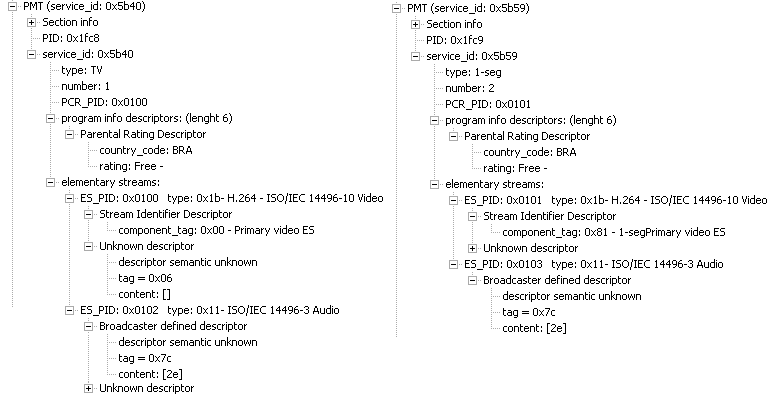
\includegraphics[width=0.9\linewidth]{figuras/ts_parser_tve_remux_pmt.png}
\\Source: The author.
\label{fig:ts_parser_tve_remux_pmt}
\end{figure}

In \autoref{fig:ts_parser_tve_remux_nit} the TS Parser is analysing the NIT of the remultiplexed TS. Since the table is too long, it was split in two parts as shown by the arrow. From the network descriptors tree, it is seen that the default network name was used in the Network Name Descriptor. The parser lacks the syntax of the System Management Descriptor. Further in the tree, one sees the value ZYA730 as the Original Network ID, the value that was passed as a parameter to FFmpeg.

Within the TS descriptors, the TS name holds the same name of the network, as defined by the SBTVD standard. In the Transmission loop, the two services have their modulation schemes detailed, as well as the service types, numbers and IDs. In the rightmost part of \autoref{fig:ts_parser_tve_remux_nit}, the Partial Reception Descriptor points that service \texttt{0x5B59} is for 1-Segment reception. Finally, the Terrestrial System Delivery Descriptor carries many of the options passed to FFmpeg, all according to the expected.

\begin{figure}[!h]
\centering
\caption{TS Parser analysing NIT of remultiplexed TS.}
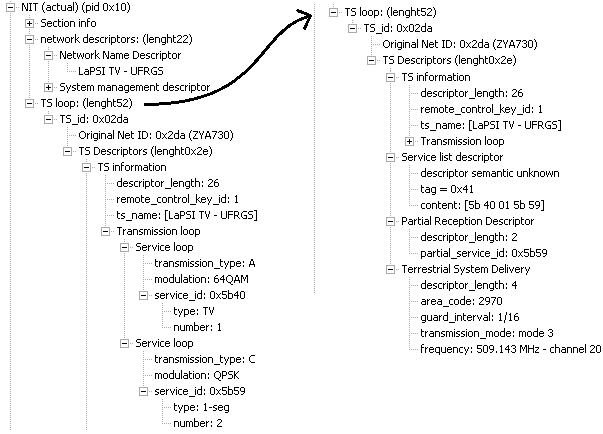
\includegraphics[width=0.9\linewidth]{figuras/ts_parser_tve_remux_nit.png}
\\Source: The author.
\label{fig:ts_parser_tve_remux_nit}
\end{figure}

In \autoref{fig:ts_parser_tve_remux_sdt} the TS Parser is analysing the SDT of the remultiplexed TS. Once again the service IDs and service types are shown, as well as the EIT scheduling flags indicating that there is neither EPG information nor EIT tables. The Service Descriptors show the service names, providers and service types.

\begin{figure}[!h]
\centering
\caption{TS Parser analysing SDT of remultiplexed TS.}
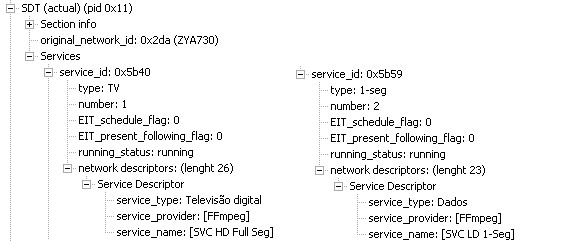
\includegraphics[width=0.9\linewidth]{figuras/ts_parser_tve_remux_sdt.png}
\\Source: The author.
\label{fig:ts_parser_tve_remux_sdt}
\end{figure}

After this complete analysis among the PSI/SI tables generated by the code developed in the project, it can be seen that all the transmitted tables and descriptors are compliant to the standard and contain valid information. Also, the information in the tables is readable by the receptors as will be seen next. The EIT table and its descriptors, not yet implemented, did not block the system functionalities. The TOT table is currently presenting errors in operation and although it was generated, it was not broadcasted.

The same sequence of tests of \autoref{retransmitting} was carried out for this Transport Stream. The results were similar as in the other tests, which is why the tables with results are not presented. Instead, some pictures were taken to illustrate the system working.

\autoref{fig:video_audio_both} shows a scene with a dB meter close to the TV speaker. In the left picture are being transmitted PAT, PMTs, NIT, SDT and video ES, but no audio ES; the audio level is 61dB. In the right picture the audio ES is sent along with the other PIDs and the level increases (to 71dB), as expected.

In \autoref{fig:info_with_without_sdt} it can be seen the effect of sending the SDT into the Transport Stream. In the left side, there is PAT, PMT, NIT but no SDT, and therefore there is no name next to the virtual channel number. In the right, on the other hand, the SDT is sent and the name "SVC HD Full Seg" is shown, which is the default name configured by the C macros in FFmpeg, as expected.

In the left side of \autoref{fig:cell_with_sdt}, the reception on the cell phone can be seen. Overlapped to the video is the channel list with the selected virtual channel '1' and the network name describing the channel. In the right side, a manual tuning is being performed in the channel 20 of the TV and no ESs nor the SDT are being sent, only PAT, PMTs and NIT. It can be seen that the channel name is empty but there is a "good" reception level. The "Channels found" flag indicates that PAT and PMT for the HD service are present, but the blue screen points that there is no ESs to be decoded.

\begin{figure}[!h]
\centering
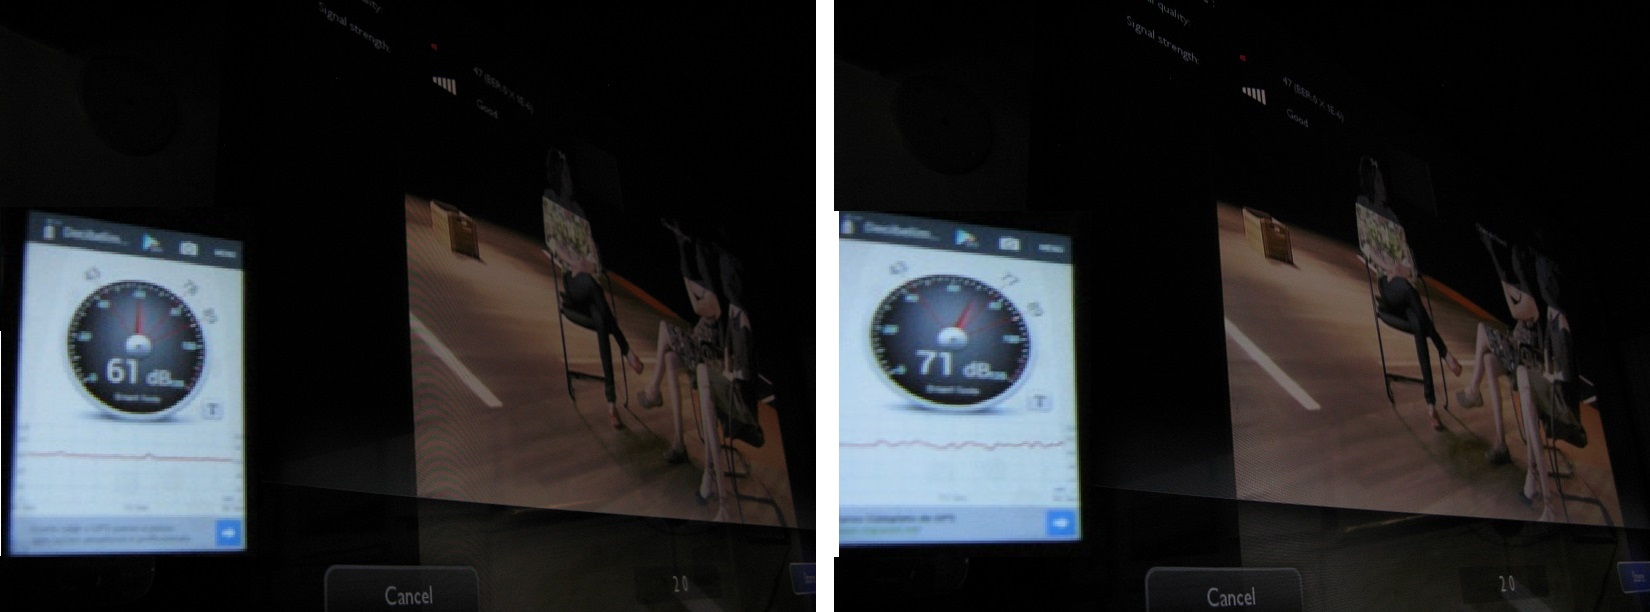
\includegraphics[width=0.9\linewidth]{figuras/video_audio_both.jpg}
\\Source: The author.
\caption{Reception of video with and without audio.}
\label{fig:video_audio_both}
\end{figure}

\begin{figure}[!h]
\centering
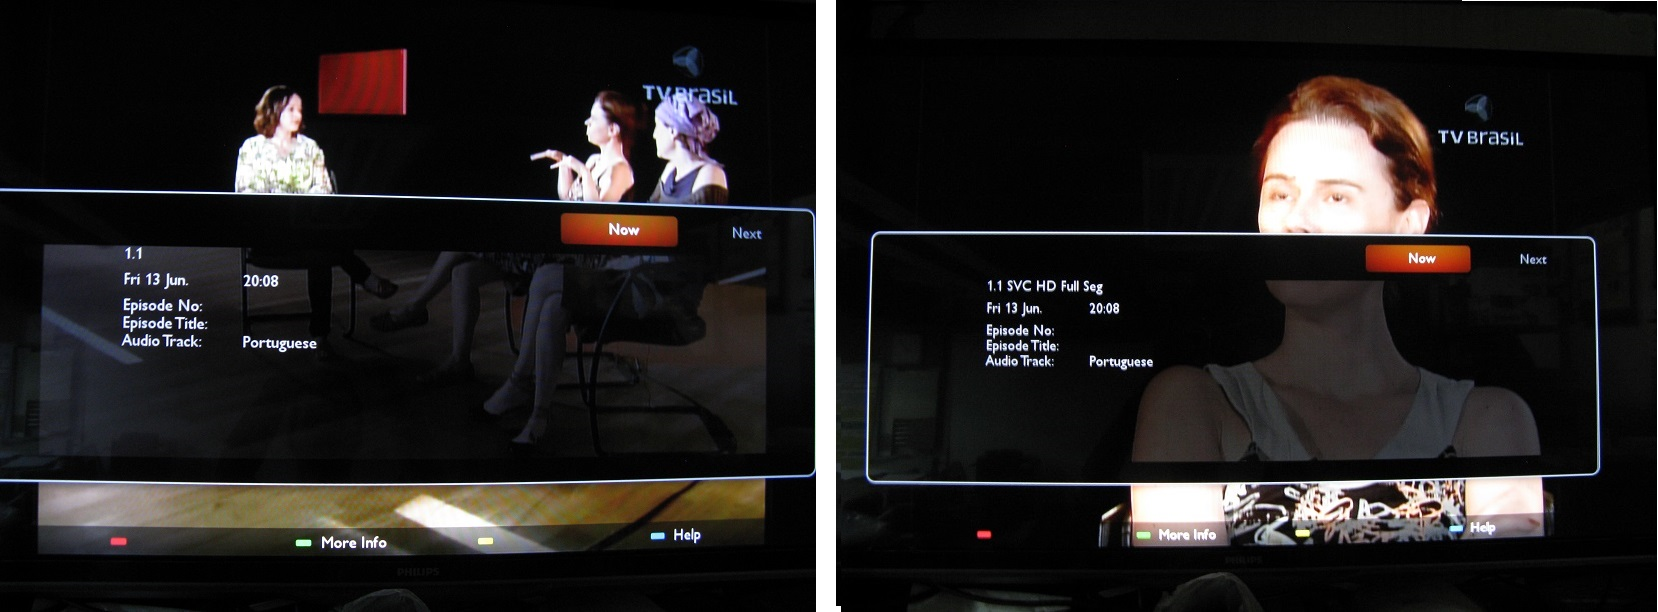
\includegraphics[width=0.9\linewidth]{figuras/info_with_without_sdt.jpg}
\\Source: The author.
\caption{Service information with and without SDT.}
\label{fig:info_with_without_sdt}
\end{figure}

\begin{figure}[!h]
\centering
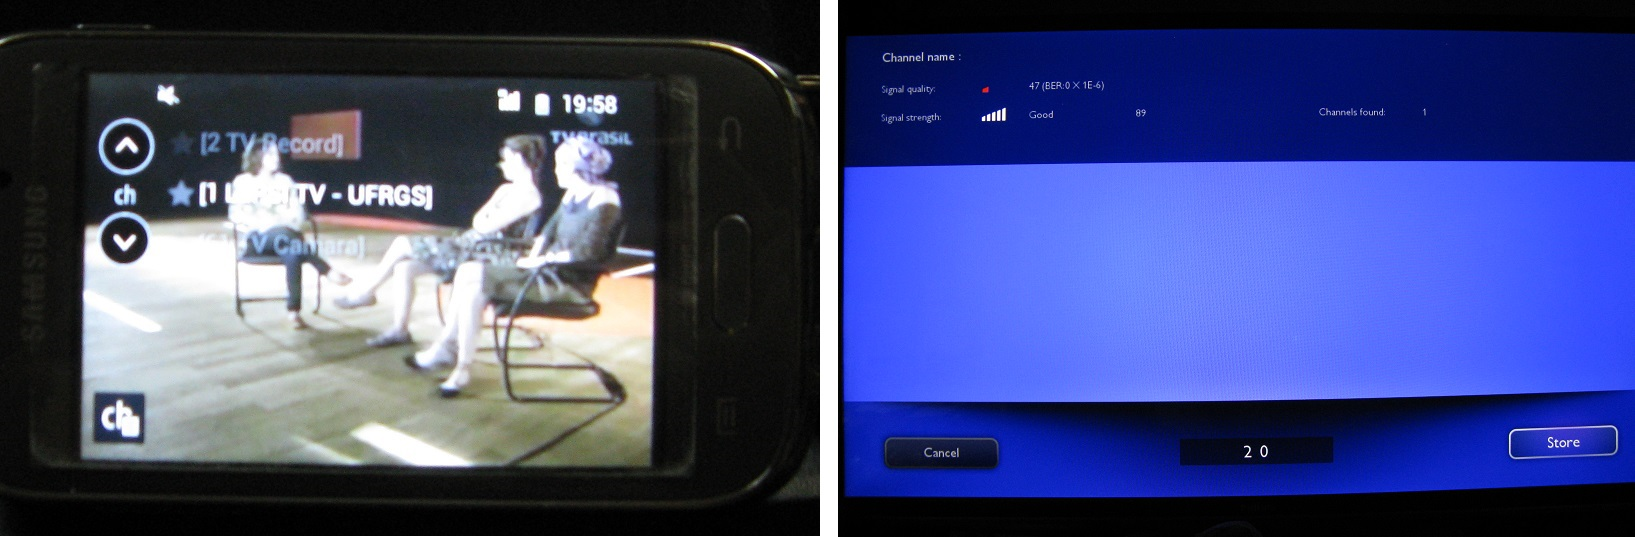
\includegraphics[width=0.9\linewidth]{figuras/cell_with_sdt.jpg}
\\Source: The author.
\caption{Reception in the Cell Phone and TV manual tuning.}
\label{fig:cell_with_sdt}
\end{figure}

%% ---
%
%\lipsum[24]

% ----------------------------------------------------------
% Finaliza a parte no bookmark do PDF
% para que se inicie o bookmark na raiz
% e adiciona espaço de parte no Sumário
% ----------------------------------------------------------
\phantompart

% ---
% Conclusão (outro exemplo de capítulo sem numeração e presente no sumário)
% ---
\chapter[Conclusions and Future Development]{Conclusions and Future Development}
%\addcontentsline{toc}{chapter}{Conclusions and Future Development}
% ---

%Intro sobre o tema

Television is the most widespread communication media in Brazil, terrestrial broadcasts cover up to 70\% of the population and people rely on television to fulfil their needs of information and entertainment. Differently than Internet, TV has roughly a unidirectional communication channel. With the growing Internet coverage, people are discovering the benefits of interactivity, which is impossible with analog television systems. Interactivity is possible if multiple data can be sent to the receiver, and the options presented to the user. By combining TV coverage to interactivity, social inclusion of remote or poor areas can be promoted. Several projects are already in development, such as the Brasil 4D application that delivers lists of job vacancies and allows users to schedule medical appointments.

Also, paid TV systems deliver high-quality video and audio contents, and subscriptions are becoming cheaper every year. There is a strong risk that, without the migration of free to air analog television to a high-quality digital system, the broadcasters will loose their audience to paid TV. It is technically not feasible to broadcast multiple TV programs or increase media quality within the existing analog channels. It is therefore necessary to adopt a digital transmission system, which provides the solution to both technical issues pointed out.

After years of discussions, the Brazilian consortium decided to base our digital television system, SBTVD-T, in the one made by the Japanese, ISDB-T. The technical aspects that led towards this choice instead of the others were the lower power consumption due to better modulation schemes and the possibility to broadcast to mobile devices as well as fixed devices within the same physical channel.

%Objetivos e como foram alcançados
%	4 objetivos do projeto? Talvez seja melhor dizer o que é o objetivo do cliente

The purpose of this study arose from the need for a tool to test the set-top box that is being developed in the Signal Processing Laboratory. There was no available tool to multiplex and broadcast the reference elementary streams, necessary to test the reception and decoding of the set-top-box. Hence, the objective of the project was to develop a flexible and free tool that allows for the transmission of multimedia streams according to the Brazilian standard.

%Metodologia (implementar modificações em ferramenta existente) com alguns resultados
%	experimentação, testes(ferramentas de teste gratuitas), leituras de documentação das ferramentas

To achieve this, it was necessary to study the standards ISO/IEC13818-1 and NBR15603. After some research looking for similar solutions that already existed, FFmpeg was found to be very easily modifiable, and was chosen as starting point of development. As methods to validate the development, a set of four receivers were used, as well as tools to analyse the generated bitstreams.

%Discussão sobre as variáveis, alguma dificuldade 
%	lack of documentation for the tool (kbps -> bps) muxrate

Although the code of FFmpeg was well commented, the lack of documentation for the tool led to several misuses at first tests. For example, there was no indication of the unit of the option muxrate and it was supposed to be kbps at first. After wrongly generated streams, it was realized that the unit was actually bps. Also, the LATM flag in the multiplexer does not really encapsulate the audio stream in LATM, it only sets the stream type in the PMT stream descriptor. This was discovered after having no audio reception in the EiTV set-top-box receiver while there was audio in the Philips TV receiver. This is probably due to the fact that only the TV has an audio decoder compliant to DTV standards other than SBTVD.

%Experimentos que poderiam ter sido realizados com a ferramenta do jeito como está	
%	codificação de ES de video usando quadros de refereência
	
Additionally to the tests that were already performed, extra experimentations can be done by applying reference video frames in the multiplexer input. The current development status allows that. Also, the encoding and multiplexing steps that are done separately could be combined into one, so that the same video input could generate both the HD and 1-Segment services.
	
%Resultados: funciona? o que funciona dos targets iniciais? multiservice, sync, sbtvd compliance. .tudo? parte? o que falta?
%	EIT nao foi feita, TOT nao funciona
%	consequencias para o projeto do set top box. agora será possível transmitir videos de referencia

Looking back to the objectives defined at the introductory chapter, it can be seen that the proposed tasks were all accomplished. The project delivers a tool which is compliant to the SBTVD standard, transmits video and audio in synchronization and allows multiple services to be broadcasted. The compliance to SBTVD and multiple service support are the two features added by this project. Timing functionalities already existed, although no one in the lab could dedicate enough effort to get it to work before.

The SBTVD compliance was achieved by adding the System Information tables which were not present in the original FFmpeg software. The Network Information Table is being created correctly. This is affirmed because in blind scans the receivers are capable of identifying the channel in their presence. Without it, though, the channel is not identified. The Service Description Table is also correct, as the receivers manage to show the service names when they receive the table.

The analyses carried out with the generated streams show the formation of almost all descriptors, the exceptions are those that the analysers can not decode. All the program and system descriptors added are being correctly interpreted by TS Analyser and TS Parser, as was shown in the tests described in previous chapters.

The SBTVD compliance is not yet fullt implemented, though. Even if it was proven that the multiplexed stream can be received by the devices and they manage to correctly decode the streams, the Event Information Table, which is mandatory, is not yet implemented. This table is not responsible for any tuning, demodulation of decoding tasks, it is only informational and that is why it was left to further development. The system works without it.

Besides, the Time Offset Table and its mandatory descriptor were implemented as well, but when they were transmitted the time information in the receivers was not updated as indicated in the table all the times. Not much time was dedicated until now to understand why this issue happens, because the multiplexer works without this information. There is no relation between current time display and presentation of the streams in sync.

Most of all, the parts which are not yet implemented are described in the theoretical chapters and can be developed with little effort, using the FFmpeg framework and taking profit of some of the algorithms described by the author.

Future development in this project can be done to turn the interface of the tool more user-friendly. It is possible to create a graphical interface with lists of valid parameter values and the status of the multiplexing process. Additionally, one key feature yet to be implemented is the second transmission profile to allow the creation of transport streams with more than just two services. The profile 2 is already defined and described in the text, and excerpts of code can be reused to implement this feature.

% futuras implementações. o que faria se tivesse mais tempo?
	% enriquecer a interface com o usario
	% fazer o código e testar outros profiles(profile 2 nao implementado)
	% EIT nao ta feita, TOT nao funciona.



% ----------------------------------------------------------
% ELEMENTOS PÓS-TEXTUAIS
% ----------------------------------------------------------
\postextual
% ----------------------------------------------------------

% ----------------------------------------------------------
% Referências bibliográficas
% ----------------------------------------------------------
\bibliography{abntex2-modelo-trabalho-academico}

% ----------------------------------------------------------
% Glossário
% ----------------------------------------------------------
%
% Consulte o manual da classe abntex2 para orientações sobre o glossário.
%
%\glossary

% ----------------------------------------------------------
% Apêndices
% ----------------------------------------------------------

% ---
% Inicia os apêndices
% ---
\begin{apendicesenv}

% Imprime uma página indicando o início dos apêndices, Documento ou texto elaborado pelo autor
\partapendices

\chapter{Modulation aspects of the SBTVD Standard}
\label{modulation}
% ---
In ISDB-T, a UHF channel is split into 13 frequency segments. The narrow-band receivers, which are capable of decoding only the central channel frequency(or segment), is commonly called a 1-segment receiver. The wide-band receivers, that can decode all the 13 frequency segments, are called full-segment decoders. \autoref{fig:ISDB-T_CH_Seg_Prog_allocation} shows the segment distribution inside a channel. 'S0' is the central segment for narrow-band tuners. 'S1' to 'S12' are the other segments. As narrower the band, as smaller is the amount of information that can be sent through it. 1-Segment receivers are used in mobile devices, and are capable of receive low definition video only, along with one single audio stream. Full-segment receivers are used in fixed devices, such as Full-HD TVs, and are capable of decode high definition video along with multiple audio streams.

The modulation schemes usually used in 'S0' are different than the ones of the other segments. Since 1-segment TV is targeted for mobile devices, the signal reach should be higher and at most a small dipole antenna is availlable, then QPSK modulation is used. For the other segments, the amount of data is much higher, and customers don't mind to have an amplified antenna attached to the back of their TV, so less robust modulation is applied, such as 64QAM. 

\begin{figure}
\centering
\caption{ISDB-T channel, segment and program allocation.}
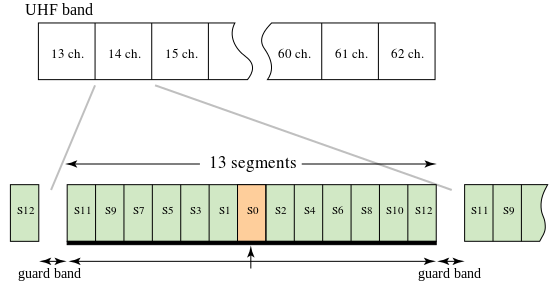
\includegraphics[width=0.8\linewidth]{figuras/ISDB-T_CH_Seg_Prog_allocation.png}
\\ Source: UnLiM, derived from Namazu-tron, obtained in Wikipedia \cite{ISDB_wiki}
\\ Licensed under Creative Commons Attribution-Share Alike 3.0 via Wikimedia Commons
\label{fig:ISDB-T_CH_Seg_Prog_allocation}
\end{figure}

% ----------------------------------------------------------
\chapter{Excerpts of code in C language}

The following lists present either code developed by the author or parts of the existent code used throughout the text to illustrate the functioning of the tool.

\begin{minipage}{\linewidth}
\begin{lstlisting}[caption={Excerpt of MpegTSWrite structure}, label={lst_MpegTSWrite}]
typedef struct MpegTSWrite {
...
MpegTSSection pat;
MpegTSSection sdt;
MpegTSService **services;
...
int nb_services;
...
int mux_rate;
...
int service_id;
int pmt_start_pid;
...
}MpegTSWrite;
\end{lstlisting}
\end{minipage}

\begin{minipage}{\linewidth}
\begin{lstlisting}[caption={Example of input option}, label=lst_input_option]
{ "mpegts_transport_stream_id", "Set transport_stream_id field.", offsetof(MpegTSWrite, transport_stream_id), AV_OPT_TYPE_INT, {.i64 = 0x0001 }, 0x0001, 0xffff, AV_OPT_FLAG_ENCODING_PARAM}
\end{lstlisting}
\end{minipage}

\begin{minipage}{\linewidth}
\begin{lstlisting}[caption={Excerpt of MpegTSSection structure}, label=lst_MpegTSSection]
typedef struct MpegTSSection {
	int pid;
	int cc;
	void(*write_packet)(struct MpegTSSection *s, const uint8_t *packet);
	void *opaque;
} MpegTSSection;
\end{lstlisting}
\end{minipage}

\begin{minipage}{\linewidth}
\begin{lstlisting}[caption={Excerpt of MpegTSService structure}, label=lst_MpegTSService]
typedef struct MpegTSService {
MpegTSSection pmt; 
int sid; 
char *name;
char *provider\hspace{0.1mm}\_\hspace{0.1mm}name;
int pcr\hspace{0.1mm}\_\hspace{0.1mm}pid;
...
}MpegTSService;
\end{lstlisting}
\end{minipage}

\begin{minipage}{\linewidth}
\begin{lstlisting}[caption={Excerpt of MpegTSWriteStream structure}, label=lst_MpegTSWriteStream]
typedef struct MpegTSWriteStream {
struct MpegTSService *service;
int pid;
int cc;
...
}MpegTSWriteStream;
\end{lstlisting}
\end{minipage}

\begin{minipage}{\linewidth}
\begin{lstlisting}[caption={Excerpt of multiple services creation algorithm.}, label={}]
    provider_name = provider ? provider->value : DEFAULT_PROVIDER_NAME;
	calculated_HD_service_ID = 0x0000;
	calculated_HD_service_ID = ( ts->onid & 0x7FF ) << 5 | 0x0 << 3 | 0x0;
	service = mpegts_add_service(ts, calculated_HD_service_ID, provider_name, "SVC HD Full Seg");
	service->pmt.write_packet = section_write_packet;
	service->pmt.opaque = s;
	service->pmt.cc = 15;

	calculated_LD_service_ID = 0x0000;
	calculated_LD_service_ID = ( ts->onid & 0x7FF ) << 5 | 0x3 << 3 | 0x1;
	service = mpegts_add_service(ts, calculated_LD_service_ID, provider_name, "SVC LD 1-Seg");
	service->pmt.write_packet = section_write_packet;
	service->pmt.opaque = s;
	service->pmt.cc = 15;
	
	ts->final_nb_services = 2;
\end{lstlisting}
\end{minipage}

\begin{minipage}{\linewidth}
\begin{lstlisting}[caption={Created macros.}, label={lst_macros}]
#define DEFAULT_NETWORK_NAME    "LaPSI TV - UFRGS"
#define DEFAULT_COUNTRY_CODE    "BRA"
#define DEFAULT_NID		0x0640
#define SDT_RETRANS_TIME 500
#define NIT_RETRANS_TIME 50
#define TOT_RETRANS_TIME 100
\end{lstlisting}
\end{minipage}

\begin{minipage}{\linewidth}
\begin{lstlisting}[caption={Pointer assignment algorithm.}, label={lst_pointer_assignment}]
q = data;
desc_len_ptr = q;
q += 2;

*q++ = 0x40;
putstr8(&q, DEFAULT_NETWORK_NAME);

*q++ = 0xFE;
sys_mgmt_desc_length_ptr = q;
*q++;
*q++ = 0x03;
*q++ = 0x01;
\end{lstlisting}
\end{minipage}

%%
\chapter{Class diagram for AVFormatContext structure}
\label{avformatcontext_class_diagram}

The class diagram for AVFormatContext is split into three parts because it is too big to fit one single page. The parts are supposed to be concatenated side by side, so that the lines representing the relations between classes match.

\begin{figure}[!hb]
\centering
\caption{Class diagram for AVFormatContext structure, part 1.}
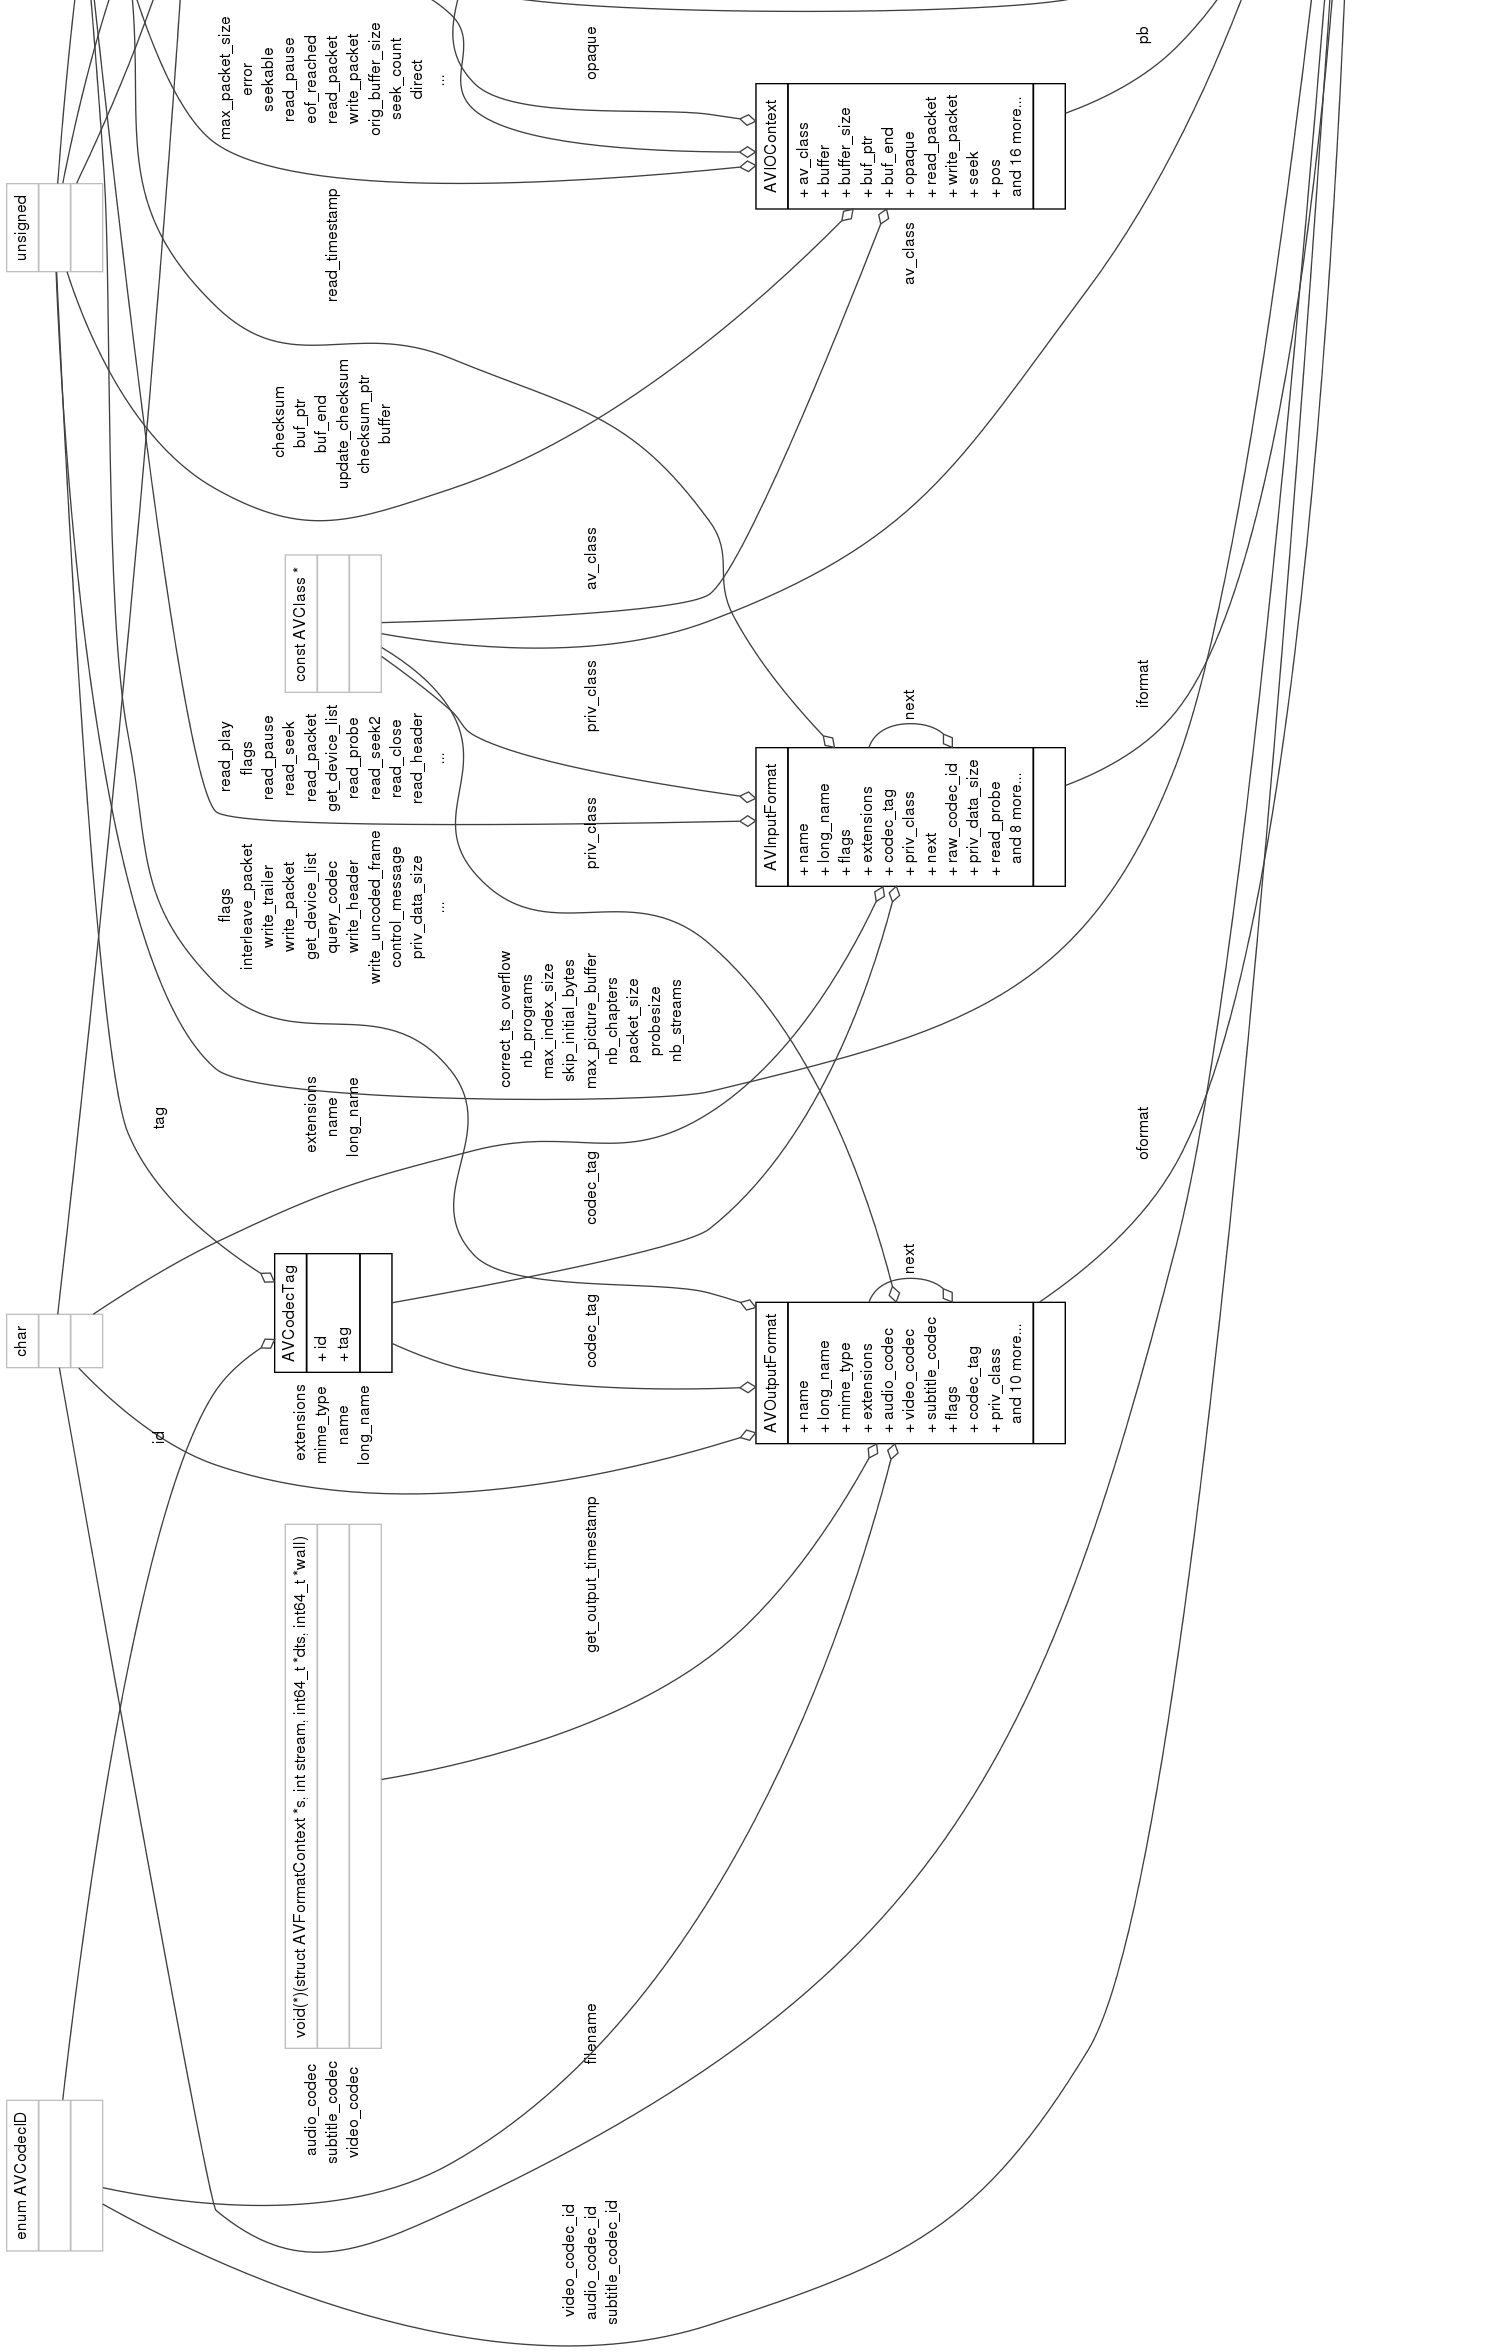
\includegraphics[width=0.9\linewidth]{figuras/structAVFormatContext__coll__graph_1.png}
\\Source: Automatically generated with Doxygen from the source code.
\label{fig:structAVFormatContext__coll__graph_1}
\end{figure}

\begin{figure}[!hb]
\centering
\caption{Class diagram for AVFormatContext structure, part 2.}
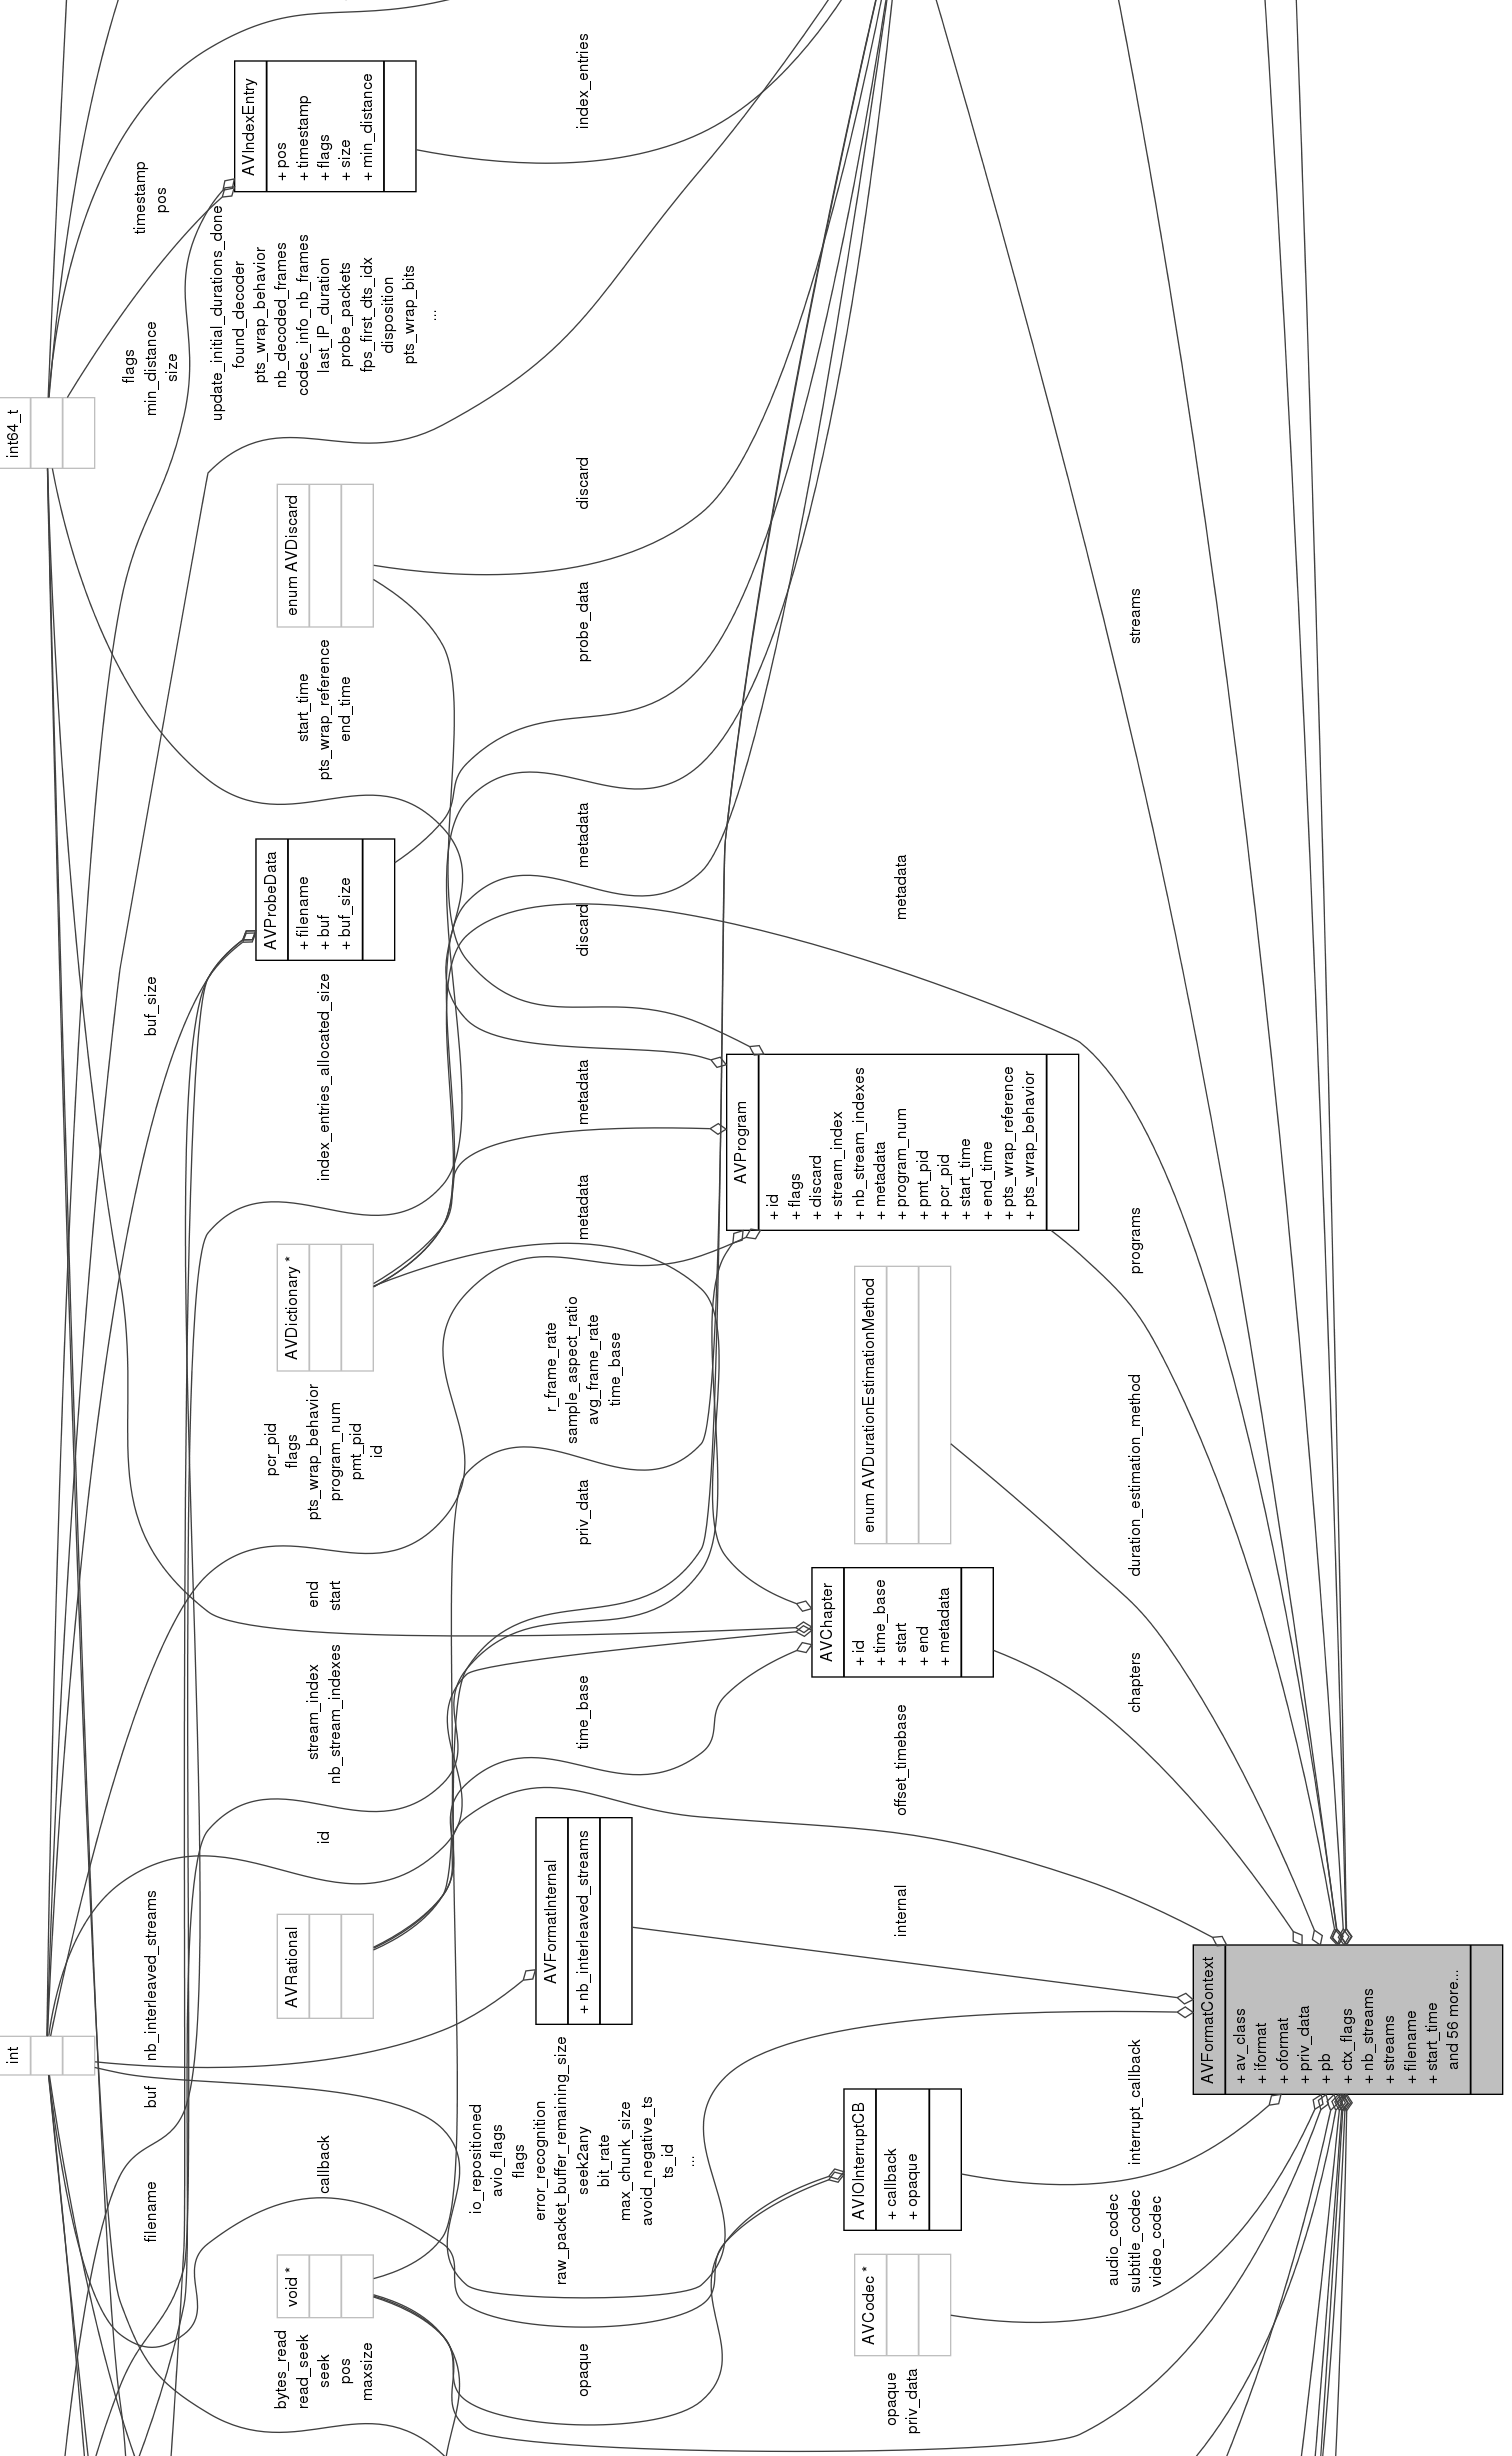
\includegraphics[width=0.9\linewidth]{figuras/structAVFormatContext__coll__graph_2.png}
\\Source: Automatically generated with Doxygen from the source code.
\label{fig:structAVFormatContext__coll__graph_2}
\end{figure}

\begin{figure}[!hb]
\centering
\caption{Class diagram for AVFormatContext structure, part 3.}
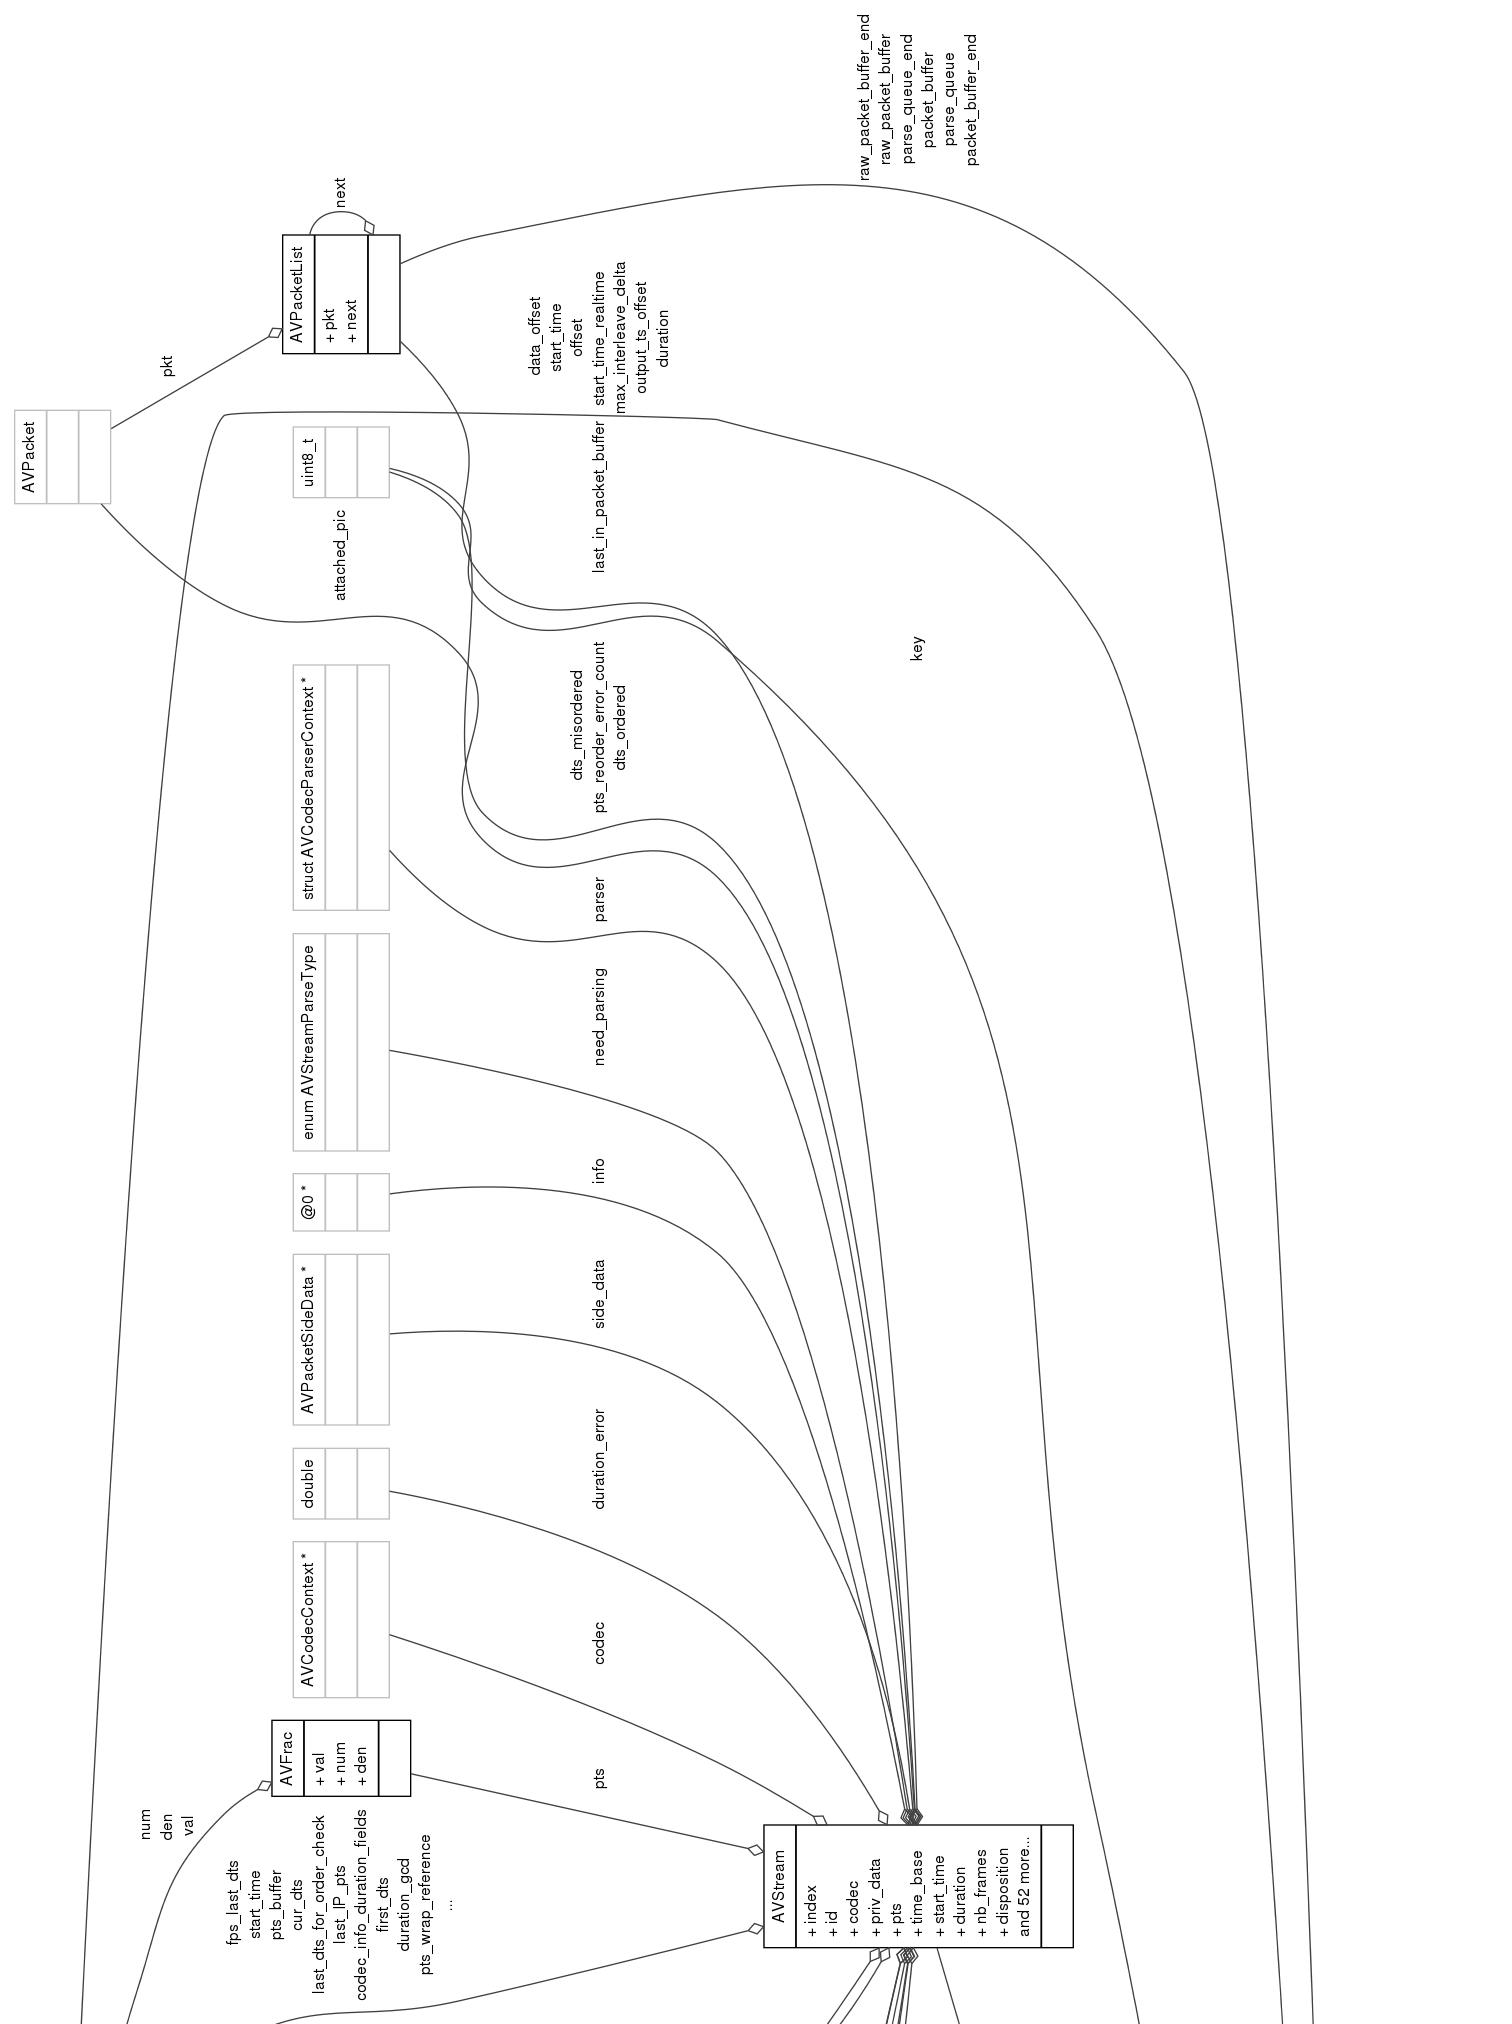
\includegraphics[width=0.9\linewidth]{figuras/structAVFormatContext__coll__graph_3.png}
\\Source: Automatically generated with Doxygen from the source code.
\label{fig:structAVFormatContext__coll__graph_3}
\end{figure}

%%


\chapter{Analyses of PSI tables}
\label{pat_pmt_analysis}

As the first example, consider \autoref{fig:TSAnalyser_close_PAT}, that shows the display of a TS Analyser when a PAT table section is analysed. The field \textit{table id} indicates \texttt{0x00}, which is the PAT code according to \autoref{fig:tab_psi_tables_ids}. The pair \textit{program\hspace{0.1mm}\_\hspace{0.1mm}number} \texttt{0} and \textit{program\hspace{0.1mm}\_\hspace{0.1mm}map\hspace{0.1mm}\_\hspace{0.1mm}PID} \texttt{16} is unique and its presence indicates that the NIT table is present and is carried in the PID \texttt{16}. It's unique because, according to the ISO standard, a program number \texttt{0} always indicates the NIT PID, and the NIT table shall always use the PID \texttt{16}, \citeonline[2.4.4.3]{ISO}. The other pairs indicate that there are two programs in the transport stream, with program numbers \texttt{23104} and \texttt{23129}. Each of these programs have their PMTs allocated in the PIDs \texttt{257} and \texttt{8136}, respectively. In the \autoref{PMT}, it will be seen how these values are taken into account.

\begin{figure}[!hb]
\centering
\caption{TS Analyser output showing a PAT Table.}
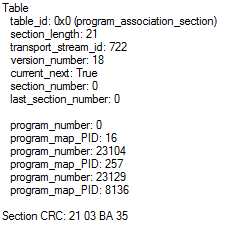
\includegraphics[width=0.4\linewidth]{figuras/TSAnalyser_close_PAT.png}
\\Source: Reproduction of the MPEG TS Analyser software.
\label{fig:TSAnalyser_close_PAT}
\end{figure}

\autoref{fig:TSAnalyser_close_PMT}, that follows, shows a snapshot of the analyser output for a PMT table. In the example, the \textit{program number} is \texttt{23104}, the table ID corresponding to the PMT is \texttt{0x02} (as defined by ISO13818-1) and the PCR information is carried in the PID (PCR\hspace{0.1mm}\_\hspace{0.1mm}PID) \texttt{256d}. Yet, from \autoref{fig:TSAnalyser_close_PMT_TS_Header}, it can be seen at the TS Header that the PID carrying the PMT table is number \texttt{257}, as indicated by the PAT table analysed before.

By analysing both \autoref{tab_ISOESTypes} and \autoref{fig:TSAnalyser_close_PMT}, one may notice that the stream types and PIDs that come after the PCR information match: the ES with PID \texttt{273} is H.264 video and the ESs with PIDs \texttt{274} and \texttt{275} are AAC/LATM audio streams, which means that there are two audio streams. The stream with type \texttt{6d} and PID \texttt{288} is the subtitle / closed captions stream. Later on this chapter the descriptors shown here will be discussed.

\begin{figure}[!hb]
\centering
\caption{TS Analyser output showing a PMT Table.}
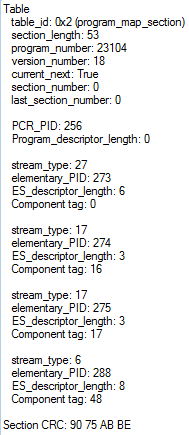
\includegraphics[width=0.4\linewidth]{figuras/TSAnalyser_close_PMT.png}
\\Source: Reproduction of the MPEG TS Analyser software.
\label{fig:TSAnalyser_close_PMT}
\end{figure}

\begin{figure}[!hb]
\centering
\caption{TS Analyser output showing the TS Header info for the PMT Table.}
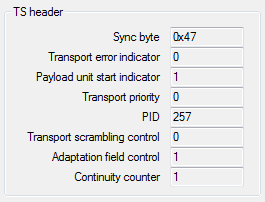
\includegraphics[width=0.4\linewidth]{figuras/TSAnalyser_close_PMT_TS_Header.png}
\\Source: Reproduction of the MPEG TS Analyser software.
\label{fig:TSAnalyser_close_PMT_TS_Header}
\end{figure}


% ----------------------------------------------------------
%\lipsum[55]

\end{apendicesenv}
% ---


% ----------------------------------------------------------
% Anexos
% ----------------------------------------------------------

% ---
% Inicia os anexos, Documento ou texto NÃO elaborado pelo autor
% ---
\begin{anexosenv}

% Imprime uma página indicando o início dos anexos
\partanexos

% ---

% ---
%\chapter{Cras non urna sed feugiat cum sociis natoque penatibus et magnis dis
%parturient montes nascetur ridiculus mus}
% ---

%\lipsum[31]

% ---
\chapter{Tables from ISO/IEC13818-1}
\label{tables_iso}
% ---

\begin{figure}[!hb]
\centering
\caption{PSI tables names, PID numbers and contents description.}
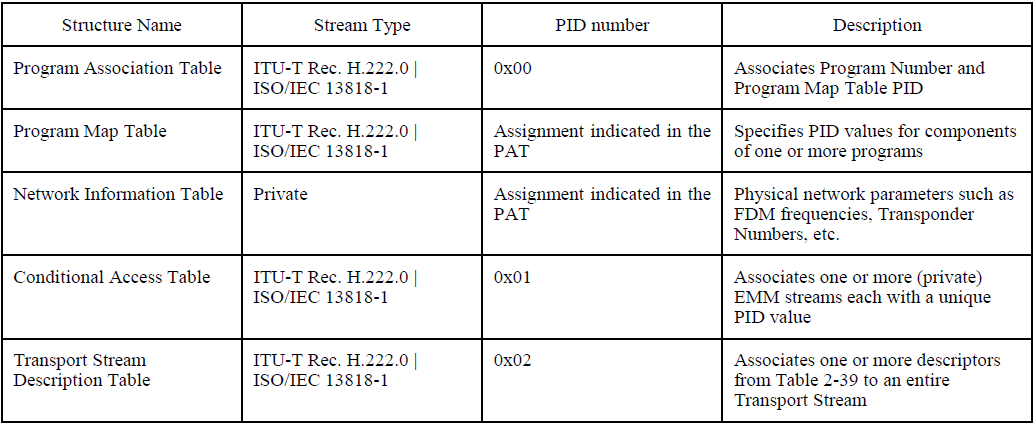
\includegraphics[width=0.7\linewidth]{figuras/tab_psi_tables_names_pids.png}
\\Source and Copyright: \citeonline[2.4.4]{ISO}
\label{fig:tab_psi_tables_names_pids}
\end{figure}

\begin{figure}[!hb]
\centering
\caption{PSI tables IDs.}
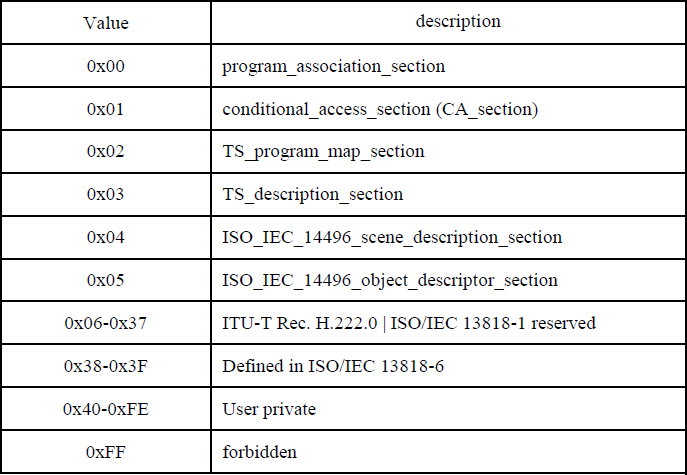
\includegraphics[width=0.7\linewidth]{figuras/tab_psi_tables_ids.png}
\\Source and Copyright: \citeonline[2.4.4.4]{ISO}
\label{fig:tab_psi_tables_ids}
\end{figure}

\begin{table}[!htpd]
\caption{Some Standardized Elementary Stream Types.}
\begin{center}
\begin{tabular}{|c|c|c|}
\hline
Decimal & Hex & Description \\
Value & Value & \\
\hline
6 & 0x06 & ITU-T Rec. H.222 and ISO/IEC 13818-1 (MPEG-2 packetized data)\\
 & & privately defined (ie, DVB subtitles/VBI and AC-3)\\
 \hline
17 & 0x11 & ISO/IEC 14496-3 (MPEG-4 LOAS multi-format framed audio)\\
 & & in a packetized stream \\
 \hline
27 & 0x1B & ITU-T Rec. H.264 and ISO/IEC 14496-10 (lower bit-rate video)\\
 & & in a packetized stream \\
\hline
\end{tabular}
\label{tab_ISOESTypes}
\\Source: \cite[2.4.4.9]{ISO}
\end{center}
\end{table}


\chapter{Tables from ABNT NBR15603}
\label{tables_abnt}

\begin{figure}[!hb]
\centering
\caption{PSI tables PIDs according to SBTVD standard.}
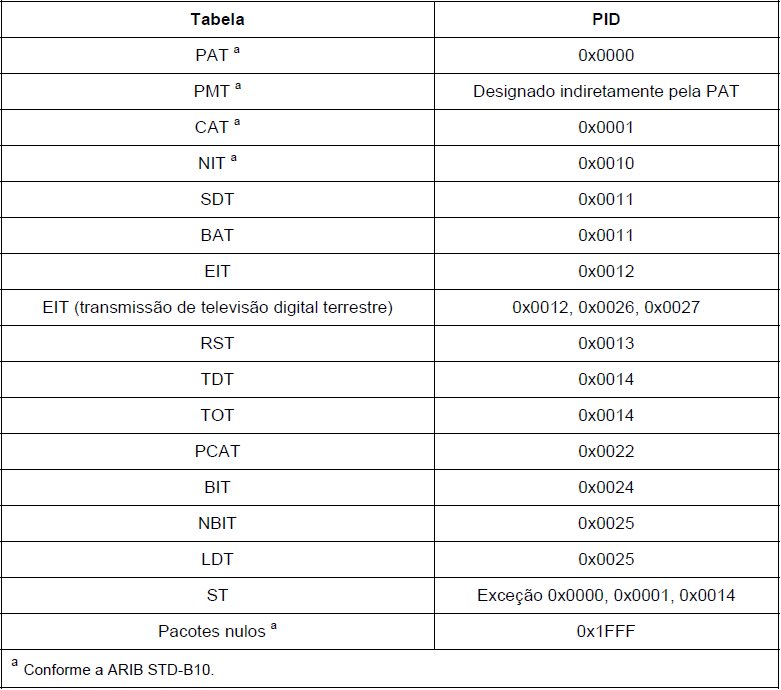
\includegraphics[width=0.7\linewidth]{figuras/tab_psi_tables_names_pids_abnt.png}
\\Source and Copyright: \citeonline[Part 2 - 7.1.4]{NBR}
\label{fig:tab_psi_tables_names_pids_abnt}
\end{figure}

\begin{figure}[!hb]
\centering
\caption{PSI tables IDs according to SBTVD standard.}
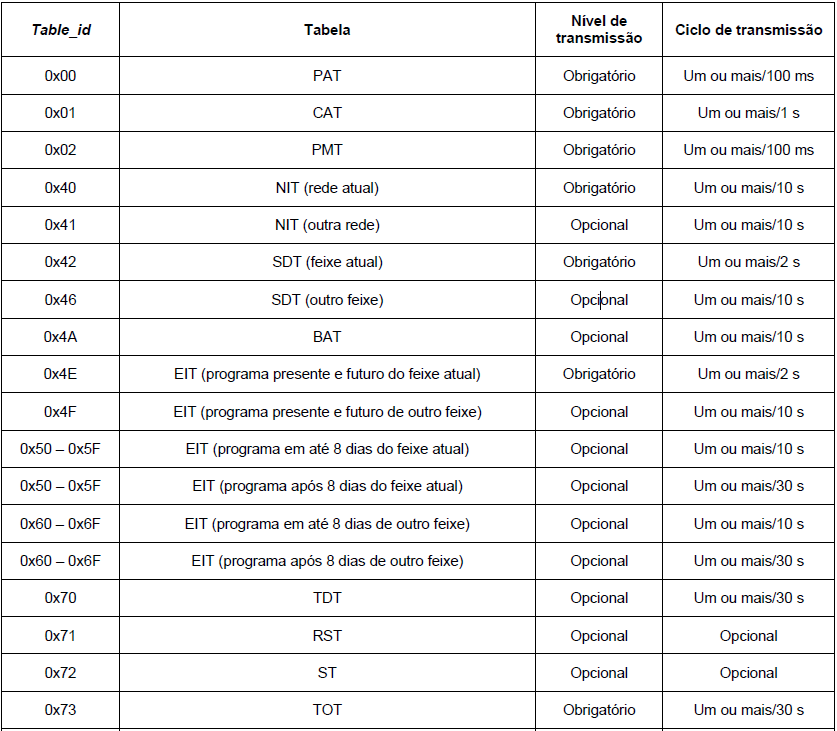
\includegraphics[width=0.7\linewidth]{figuras/tab_psi_tables_ids_level_frequency_abnt.png}
\\Source and Copyright: \citeonline[Part 2 - 7.1.4]{NBR}
\label{fig:tab_psi_tables_ids_level_frequency}
\end{figure}



\end{anexosenv}

%---------------------------------------------------------------------
% INDICE REMISSIVO
%---------------------------------------------------------------------
\phantompart
\printindex
%---------------------------------------------------------------------

\end{document}
